% From https://github.com/UWIT-IAM/UWThesis
\documentclass[print]{nuthesis}
\usepackage{amssymb, amsthm, amsmath, amsfonts}
\usepackage{wasysym}
\usepackage{mathrsfs}
% \usepackage{hyperref}
\usepackage{graphicx}
\usepackage{lineno}
\usepackage[colorinlistoftodos]{todonotes}
\usepackage{listings}
%\usepackage{breqn}
\usepackage{cancel, enumerate}
\usepackage{rotating, environ}
\usepackage{caption}
\usepackage{subcaption}
\usepackage[inline]{enumitem}
\usepackage{dirtree}

\newtheorem{thm}{Theorem}
\newtheorem{defn}{Definition}
\newtheorem{prop}{Proposition}
\newtheorem{lemma}{Lemma}
\newtheorem{cor}{Corollary}

% Syntax highlighting #22
  \usepackage{color}
  \usepackage{fancyvrb}
  \newcommand{\VerbBar}{|}
  \newcommand{\VERB}{\Verb[commandchars=\\\{\}]}
  \DefineVerbatimEnvironment{Highlighting}{Verbatim}{commandchars=\\\{\}}
  % Add ',fontsize=\small' for more characters per line
  \usepackage{framed}
  \definecolor{shadecolor}{RGB}{248,248,248}
  \newenvironment{Shaded}{\begin{snugshade}}{\end{snugshade}}
  \newcommand{\AlertTok}[1]{\textcolor[rgb]{0.94,0.16,0.16}{#1}}
  \newcommand{\AnnotationTok}[1]{\textcolor[rgb]{0.56,0.35,0.01}{\textbf{\textit{#1}}}}
  \newcommand{\AttributeTok}[1]{\textcolor[rgb]{0.77,0.63,0.00}{#1}}
  \newcommand{\BaseNTok}[1]{\textcolor[rgb]{0.00,0.00,0.81}{#1}}
  \newcommand{\BuiltInTok}[1]{#1}
  \newcommand{\CharTok}[1]{\textcolor[rgb]{0.31,0.60,0.02}{#1}}
  \newcommand{\CommentTok}[1]{\textcolor[rgb]{0.56,0.35,0.01}{\textit{#1}}}
  \newcommand{\CommentVarTok}[1]{\textcolor[rgb]{0.56,0.35,0.01}{\textbf{\textit{#1}}}}
  \newcommand{\ConstantTok}[1]{\textcolor[rgb]{0.00,0.00,0.00}{#1}}
  \newcommand{\ControlFlowTok}[1]{\textcolor[rgb]{0.13,0.29,0.53}{\textbf{#1}}}
  \newcommand{\DataTypeTok}[1]{\textcolor[rgb]{0.13,0.29,0.53}{#1}}
  \newcommand{\DecValTok}[1]{\textcolor[rgb]{0.00,0.00,0.81}{#1}}
  \newcommand{\DocumentationTok}[1]{\textcolor[rgb]{0.56,0.35,0.01}{\textbf{\textit{#1}}}}
  \newcommand{\ErrorTok}[1]{\textcolor[rgb]{0.64,0.00,0.00}{\textbf{#1}}}
  \newcommand{\ExtensionTok}[1]{#1}
  \newcommand{\FloatTok}[1]{\textcolor[rgb]{0.00,0.00,0.81}{#1}}
  \newcommand{\FunctionTok}[1]{\textcolor[rgb]{0.00,0.00,0.00}{#1}}
  \newcommand{\ImportTok}[1]{#1}
  \newcommand{\InformationTok}[1]{\textcolor[rgb]{0.56,0.35,0.01}{\textbf{\textit{#1}}}}
  \newcommand{\KeywordTok}[1]{\textcolor[rgb]{0.13,0.29,0.53}{\textbf{#1}}}
  \newcommand{\NormalTok}[1]{#1}
  \newcommand{\OperatorTok}[1]{\textcolor[rgb]{0.81,0.36,0.00}{\textbf{#1}}}
  \newcommand{\OtherTok}[1]{\textcolor[rgb]{0.56,0.35,0.01}{#1}}
  \newcommand{\PreprocessorTok}[1]{\textcolor[rgb]{0.56,0.35,0.01}{\textit{#1}}}
  \newcommand{\RegionMarkerTok}[1]{#1}
  \newcommand{\SpecialCharTok}[1]{\textcolor[rgb]{0.00,0.00,0.00}{#1}}
  \newcommand{\SpecialStringTok}[1]{\textcolor[rgb]{0.31,0.60,0.02}{#1}}
  \newcommand{\StringTok}[1]{\textcolor[rgb]{0.31,0.60,0.02}{#1}}
  \newcommand{\VariableTok}[1]{\textcolor[rgb]{0.00,0.00,0.00}{#1}}
  \newcommand{\VerbatimStringTok}[1]{\textcolor[rgb]{0.31,0.60,0.02}{#1}}
  \newcommand{\WarningTok}[1]{\textcolor[rgb]{0.56,0.35,0.01}{\textbf{\textit{#1}}}}

%% https://github.com/rstudio/rmarkdown/issues/1649
\newlength{\cslhangindent}
\setlength{\cslhangindent}{1.5em}
\newenvironment{CSLReferences}%
{\setlength{\parindent}{0pt}%
\everypar{\setlength{\hangindent}{\cslhangindent}}\ignorespaces}%
{\par}

% fix for pandoc 1.14
\providecommand{\tightlist}{%
  \setlength{\itemsep}{0pt}\setlength{\parskip}{0pt}}

%% something about tables, from https://github.com/ismayc/thesisdown/issues/122
\usepackage{calc}

%% for copyright symbol
\usepackage{textcomp}

%% to allow to rotate pages to landscape
\usepackage{lscape}
%% to adjust table column width
\usepackage{tabularx}

% suppress bottom page numbers on first page of each chapter
% because they overlap with text
\usepackage{etoolbox}
\patchcmd{\chapter}{plain}{empty}{}{}

%% for more attractive tables
\usepackage{booktabs}
\usepackage{longtable}


\usepackage{graphicx}


% Double spacing, if you want it.
\def\dsp{\def\baselinestretch{2.0}\large\normalsize}
% \dsp

% If the Grad. Division insists that the first paragraph of a section
% be indented (like the others), then include this line:
\usepackage{indentfirst}

%%%%%%%%%%%%%%%%%%
% If you want to use "sections" to partition your thesis
% un-comment the following:
%
% \counterwithout{section}{chapter}
% \setsecnumdepth{subsubsection}
% \def\sectionmark#1{\markboth{#1}{#1}}
% \def\subsectionmark#1{\markboth{#1}{#1}}
% \renewcommand{\thesection}{\arabic{section}}
% \renewcommand{\thesubsection}{\thesection.\arabic{subsection}}
% \makeatletter
% \let\l@subsection\l@section
% \let\l@section\l@chapter
% \makeatother
% 
% \renewcommand{\thetable}{\arabic{table}}
% \renewcommand{\thefigure}{\arabic{figure}}

%%%%%%%%%%%%%%%%%%


%% Stuff from https://github.com/suchow/Dissertate

% The following line would print the thesis in a postscript font

% \usepackage{natbib}
% \def\bibpreamble{\protect\addcontentsline{toc}{chapter}{Bibliography}}

\setcounter{tocdepth}{1} % Print the chapter and sections to the toc
% controls depth of table of contents (toc): 0 = chapter, 1 = section, 2 = subsection

\usepackage{natbib}


% commands and environments needed by pandoc snippets
% extracted from the output of `pandoc -s`
%% Make R markdown code chunks work
\usepackage{array}
\usepackage{amssymb,amsmath}
\usepackage{ifxetex,ifluatex}
\ifxetex
  \usepackage{fontspec,xltxtra,xunicode}
  \defaultfontfeatures{Mapping=tex-text,Scale=MatchLowercase}
\else
  \ifluatex
    \usepackage{fontspec}
    \defaultfontfeatures{Mapping=tex-text,Scale=MatchLowercase}
  \else
    \usepackage[utf8]{inputenc}
  \fi
\fi
\usepackage{color}
\usepackage{fancyvrb}


\ifxetex
  \usepackage[setpagesize=false, % page size defined by xetex
              unicode=false, % unicode breaks when used with xetex
              xetex,
              colorlinks=true,
              linkcolor=blue]{hyperref}
\else
  \usepackage[unicode=true,
              colorlinks=true,
              linkcolor=blue]{hyperref}
\fi
\hypersetup{breaklinks=true, pdfborder={0 0 0}}
\setlength{\parindent}{20pt}
\setlength{\parskip}{6pt plus 2pt minus 1pt}
\setlength{\emergencystretch}{3em}  % prevent overfull lines
\setcounter{secnumdepth}{2} %% controls section numbering, e.g. 1 or 1.2, or 1.2.3



%  ----  Text Colors  ------------------------------------------
%
% Assign colors to writers for review
%
\newcommand{\ear}[1]{{\textcolor{blue}{#1}}}
\newcommand{\svp}[1]{{\textcolor{RedOrange}{#1}}}
\newcommand{\rh}[1]{{\textcolor{Green}{#1}}}
%
\raggedright
\setlength{\parindent}{1cm}

%  --- Code chunk font size -----------------------------------------------
% https://stackoverflow.com/questions/38323331/code-chunk-font-size-in-beamer-with-knitr-and-latexhttps://stackoverflow.com/questions/38323331/code-chunk-font-size-in-beamer-with-knitr-and-latex

%% change fontsize of R code
% \let\oldShaded\Shaded
% \let\endoldShaded\endShaded
% \renewenvironment{Shaded}{\footnotesize\oldShaded}{\endoldShaded}
% 
% %% change fontsize of output
% \let\oldverbatim\verbatim
% \let\endoldverbatim\endverbatim
% \renewenvironment{verbatim}{\footnotesize\oldverbatim}{\endoldverbatim}


\begin{document}
% \linenumbers{}
%% Start formatting the first few special pages
%% frontmatter is needed to set the page numbering correctly
\frontmatter
%% from thesisdown
% To pass between YAML and LaTeX the dollar signs are added by CII
\title{HUMAN PERCEPTION OF EXPONENTIALLY INCREASING DATA DISPLAYED ON A LOG SCALE}
\author{Emily Anna Robinson}
\adviser{Susan VanderPlas and Reka Howard}
\adviserAbstract{}
\major{Statistics}
\degreemonth{August}
\degreeyear{2022}
% \copyrightpage
%%
%% For most people the defaults will be correct, so they are commented
%% out. To manually set these, just uncomment and make the needed
%% changes.
%% \college{Your college}
%% \city{Your City}
%%
%% For most people the following can be changed with a class
%% option. To manually set these, just uncomment the following and
%% make the needed changes.
%% \doctype{Thesis or Dissertation}
%% \degree{Your degree}
%% \degreeabbreviation{Your degree abbr.}
%%
%% Now that we know everything we need, we can generate the title page
%% itself.
%%
\maketitle


% \begin{abstract}
%     Log scales are often used to display data over several orders of magnitude within one graph. During the COVID-19 pandemic, we have seen both the benefits and the pitfalls of using log scales to display case counts. Three graphical experimental tasks were conducted to evaluate the impact our choice of scale has on human perception of exponentially increasing trends. The first experiment evaluates whether our ability to perceptually notice differences in exponentially increasing trends is impacted by the choice of scale. We conducted a visual inference experiment in which participants were shown a series of lineup plots (consisting of 19 null panels and 1 target panel) and asked to identify the panel that was most different from the others. Our results indicated that when there was a large difference in curvature between the target plot and null plots, the choice of scale had no impact and participants accurately differentiated between the two curves on both the linear and log scale. However, displaying exponentially increasing data on a log scale improved the accuracy of differentiating between models with slight curvature differences. An exception occurred when identifying a plot with curvature embedded in surrounding plots closely relating to a linear trend, indicating that it is easy to identify a curve in a group of lines but much harder to identify a line in a group of curves. The use of visual inference to identify these guidelines suggests that there are \emph{perceptual} advantages to log scales when differences are subtle. Our other experimental tasks focus on determining whether there are cognitive disadvantages to log scales: do log scales make it harder to make use of graphical information? We conducted a graphical task similar to the New York Times ``You Draw It'' page to test an individual's ability to use and make predictions for exponentially increasing data. We asked participants to draw a line using their computer mouse through the increasing exponential trend shown on both scales. In addition to differentiation and prediction of exponentially increasing data, we conduct an experimental task to test an individuals' ability to translate a graph of exponentially increasing data into real value quantities and extend their estimations by making comparisons. The results of our experimental tasks allow us to provide guidelines for readers to actively choose which of many possible graphics to draw, according to some set of design choices, to ensure that our charts are effective. \emph{(399 words; 350 word limit)}
% \end{abstract}

%% Optional
%% \begin{copyrightpage}
%% \end{copyrightpage}

%% Optional
% \begin{dedication}
% Dedicated to\ldots{}
% \end{dedication}

%%%%%%%%%%%%%%%%%%%
% Acknowledgments
%%%%%%%%%%%%%%%%%%%
% \begin{acknowledgments}
% Thank you to all my people!
% \end{acknowledgments}
%%%%%%%%%%%%%%%%%%%

%%%%%%%%%%%%%%%%%%%
% Grant Information
%%%%%%%%%%%%%%%%%%%
% \begin{grantinfo}
%     % Add any grant info here
% \end{grantinfo}

%%%%%%%%%%%%%%%%%%%
% ToC
%%%%%%%%%%%%%%%%%%%
\tableofcontents

%%%%%%%%%%%%%%%%%%%
% List of Figures
%%%%%%%%%%%%%%%%%%%
\listoffigures
\listoftables

%%%%%%%%%%%%%%%%%%%
% Start of the document
%%%%%%%%%%%%%%%%%%%
\mainmatter


\hypertarget{literature-review}{%
\chapter{Literature Review}\label{literature-review}}

\hypertarget{introduction-to-graphics}{%
\section{Introduction to Graphics}\label{introduction-to-graphics}}

Advanced technology and computing power have promoted data visualization as a central tool in modern data science. Unwin (2020) defines data visualization as the art of drawing graphical charts in order to display data.
Graphics are useful for data cleaning, exploring data structure, and have been an essential component in communicating information for the last 200 years (Lewandowsky \& Spence, 1989)
During the \(\text{18}^{\text{th}}\) and \(\text{19}^{\text{th}}\) centuries, governments began using graphics in order to better understand their population and economic interests (Harms, 1991; Playfair, 1801; Walker \& others, 2013).
In \cref{fig:william-playfair-trade}, Playfair (1801) visually represents the power and economic status of each European Nation in the early \(\text{19}^{\text{th}}\) century.
Circle size and numeric annotation within the circle indicate the number of square miles in each country with the number of people per square mile indicated above the circle.
The vertical bar to the left side represents the number of inhabitants (millions), and the line to the right side represents the revenue (million pounds).
Color in the original figure, not shown, identifies countries as maritime powers or powerful by land only.
The Statistical atlas of the United States (Walker \& others, 2013) used charts and graphics to display data compiled from the 1870 US census.
\cref{fig:statistical-atlas-state-population} displays the population of each state where square size represents the proportion of the states population separated into three regions representing the origin and race of the population.
The rectangle shown to the right represents the proportion of residents born in the state who have become residents of other states.
In the \(\text{20}^{\text{th}}\) century, companies began utilizing graphics to understand their mechanics and support business decisions and news sources began displaying graphics of weather forecasts as a means to communicate critical information and aid in decision-making (Chandar, Collier, \& Miranti, 2012; Yates, 1985).
Chandar, Collier, \& Miranti (2012) illustrates how AT\&T used graphics to demonstrate management's ability to optimize utilization of assets by making comparisons between their annual net telephone revenues and their returns on total assets \pcref{fig:ATandT-revenue}.
Today, we encounter data visualizations everywhere; researchers include graphics to communicate their results in scientific publications and mass media present graphics in order to convey news stories to the public through newspapers, TV, and the Web (Aisch et al., 2016; Gouretski \& Koltermann, 2007; Silver, 2020).

\begin{figure}[tbp]

{\centering 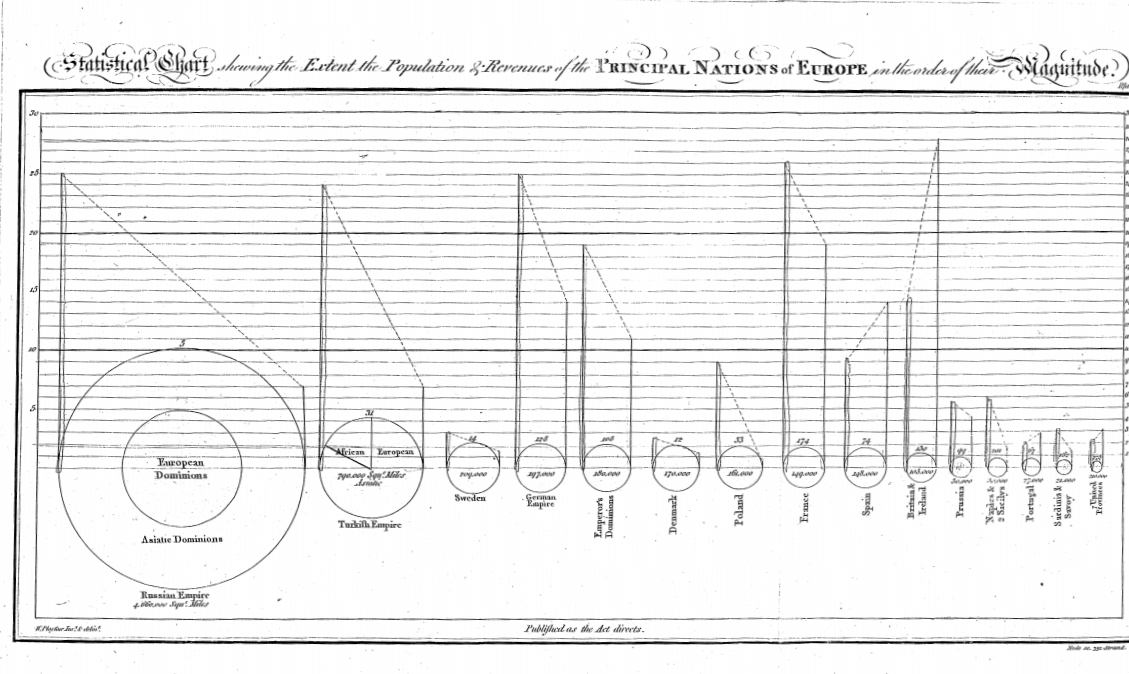
\includegraphics[width=0.75\linewidth,]{images/william-playfair-balance-trade} 

}

\caption{William Playfair's balance of trate}\label{fig:william-playfair-trade}
\end{figure}

\begin{figure}[tbp]

{\centering 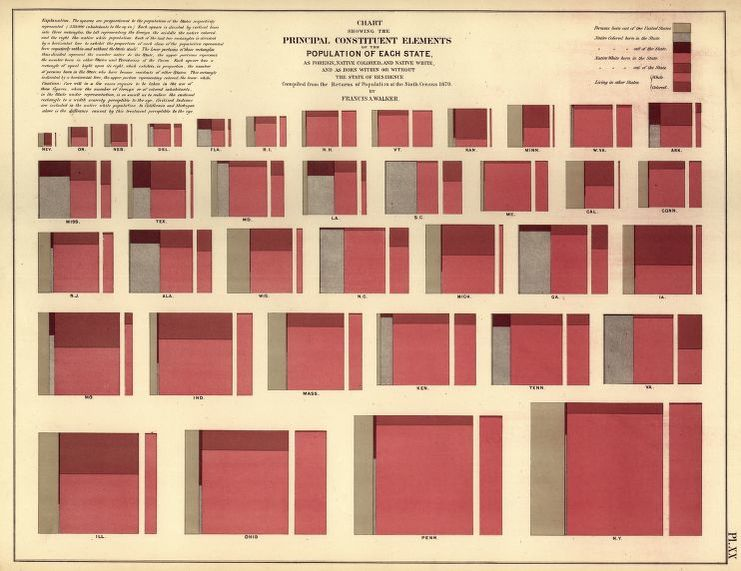
\includegraphics[width=0.75\linewidth,]{images/statistical-atlas-state-population} 

}

\caption{Statistical Atlas 1870 state population}\label{fig:statistical-atlas-state-population}
\end{figure}

\begin{figure}[tbp]

{\centering 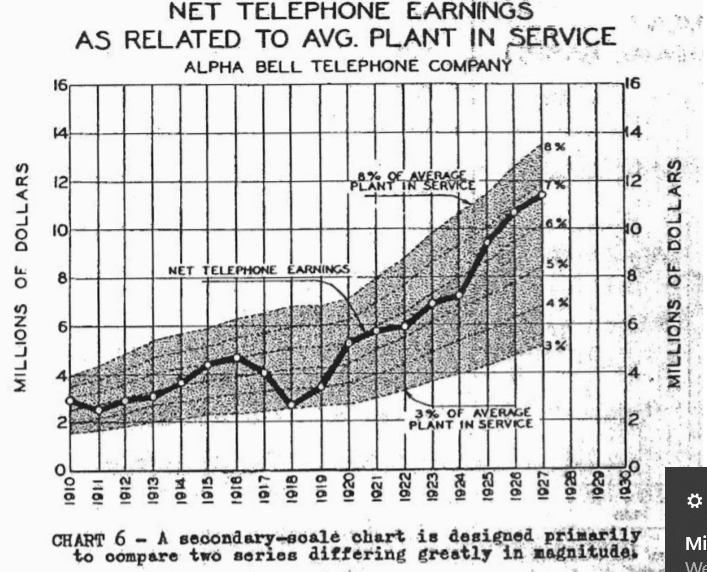
\includegraphics[width=0.75\linewidth,]{images/ATandT-revenue} 

}

\caption{AT\&T utilization of assets}\label{fig:ATandT-revenue}
\end{figure}

Although statistical graphics have become widely used and valued in science, business, and in many other aspects of life, as creators of graphics, we are too accepting of them as default without asking critical questions about the graphics we create or view (Unwin, 2020).
Vanderplas, Cook, \& Hofmann (2020) poses the general question we must ask ourselves, ``how effective is this graph at communicating useful information?''
An effective graphic accurately shows the data through the appropriate chart selection, axes and scales, and aesthetic design choices in order to successfully communicate the intended result.
\protect\hyperlink{misleading-graphics}{Section 1.2} illustrates how graphics can be misleading and ineffective at communicating the intended result by inaccurately displaying the data.

Higher quality of technology has influenced the creation, replication, and complexity of graphics as there are an infinitely many number of graphical displays and design choices that can be implemented at faster speeds with more flexibility.
The creator of a graphic makes decisions about the variables displayed, the type of graphic, the size of the graphic and the aspect ratio, the colors and symbols used, the scales and limits, and the ordering of categorical variables.
In response to the increasing number of design choices, consistent themes and higher standards are being placed on graphics.
Selecting from an extensive list of styles and choices of graphics in order to effectively communicate insights into the data is a challenging task.
A consistent concern is the lack of theory of graphics available to build on; better theory should result in better graphics.
Creators of graphics need an established set of concepts and terminology to build their graphics from so they can actively choose which of many possible graphics to draw in order to ensure their charts are effective at communicating the intended result.

Many efforts have been made to provide guidelines for graphical designs including Wilkinson's Grammar of Graphics (Wilkinson, 2012).
The grammar of graphics serves as the fundamental framework for data visualization with the notion that graphics are built from the ground up by providing a way of specifying exactly how to create a particular graph from a given data set.
Visual representations are constructed through the use of ``tidy data'' which is characterized as a data set in which each variable is in its own column, each observation is in its own row, and each value is in its own cell (Hadley Wickham \& Grolemund, 2016).
Graphics are viewed as a mapping from variables in a data set (or statistics computed from the data) to visual attributes such as the axes, colors, shapes, or facets on the canvas in which the chart is displayed.
\cref{fig:graphic-flowchart} illustrates the process of creating a graphic from a data set through the use of variable mapping, data transformations, coordinate systems, and aesthetic features (Vanderplas, Cook, \& Hofmann, 2020)
Software, such as Hadley Wickham's ggplot2 (Hadley Wickham, 2011), aims to implement the framework of creating graphics as recommended in the grammar of graphics.

\begin{figure}[tbp]

{\centering 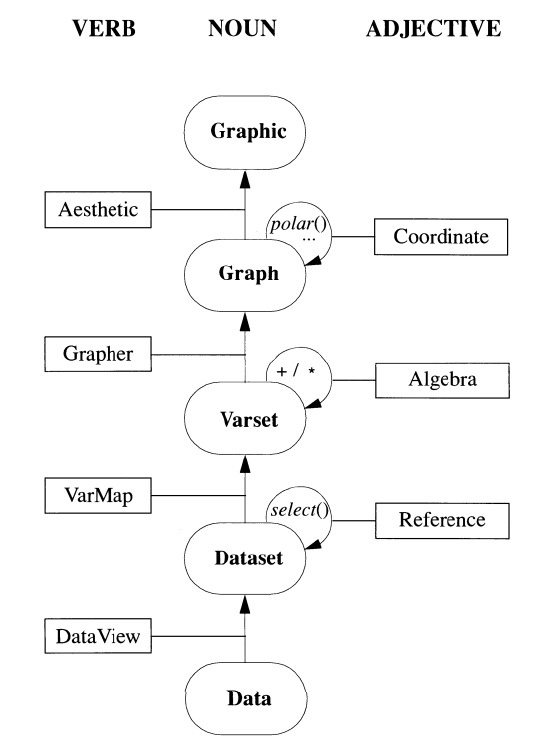
\includegraphics[width=0.5\linewidth,]{images/graphic-flowchart} 

}

\caption{Graphic flowchart}\label{fig:graphic-flowchart}
\end{figure}

Despite past attempts to improve the use of graphics in science, graphics displayed in academic research are still falling short of the standards. Gordon \& Finch (2015) evaluated 97 graphs for overall quality, based on five principles of graphical excellence including: (1) show the data clearly (2) use simplicity in design (3) use good alignment on a common scale for quantities to be compared (4) keep the visual encoding transparent (5) use graphical forms consistent with principles 1 and 4.
The authors randomly sampled 97 graphs published in A* (top 5\%) journals with work in statistics and applied science disciplines.
There were 50 graphs sampled from the most recently available issues of A* journals in applied sciences such as environmental sciences, agricultural and veterinary sciences, medical and health sciences, education, economics, and psychology.
The additional 47 graphs were randomly sampled from A* statistics journals.
Each graph was scored based on 60 features related to the five principles, such as proper axes labels.
Both authors assigned an overall quality rating (poor, adequate, good, or exemplary) to each of the graphs sampled; discrepancies in ratings were settled with discussion.
The authors rated 39\% of the 97 graphs sampled as poor, indicating there is still an astonishing lack in the quality of graphics.
More startling is the fact that the source of the graphic from an applied science or a statistics graphic had no effect on the quality of the graphic.
In order to achieve a higher standard of the graphics being presented, future work must be done to implement the academic research being conducted in graphics into practice.

\hypertarget{misleading-graphics}{%
\section{Misleading Graphics}\label{misleading-graphics}}

\hypertarget{perception-and-psychophysics}{%
\section{Perception and Psychophysics}\label{perception-and-psychophysics}}

\hypertarget{perceptual-process}{%
\subsection{Perceptual Process}\label{perceptual-process}}

In order to develop guiding principles for generating graphics effective in communication, we must first understand the basic mechanics of the human perceptual system and the biases we are vulnerable to (Goldstein \& Brockmole, 2017).
The perceptual process is a sequence of steps used to describe a how a stimulus in the environment leads to our perception of the stimulus and action in response to the stimulus \pcref{fig:perceptual-process}.
This process is broken down into sensation (Carlson, 2010) - involving simple processes that occur right at the beginning of a sensory system - and perception (Myers \& DeWall, 2021) - involving higher-order mechanisms and identified with more complex processes.

The perceptual process begins when there is a stimulus in the environment and light is reflected and focused back into the viewer's eyes.
Within the eye, the light reflected is transformed and focused by the eye's optical system and an image is formed on the receptors of the viewer's retina.
It is important to note that everything a person perceives is based not on direct contact with stimuli but on representations of stimuli that are formed on the receptors and the resulting activity in the person's nervous system.
Once light is reflected and focused, our visual receptors respond to the light and transform the light energy into electrical energy through a process called transduction.
Signals from the receptors are then transmitted through the retina, to the brain, and then within the brain where perception (what do you see?) and recognition (what is it called?) occur.
After recognition, viewers take some sort of motor action; for example, move closer to the object.
The perceptual process is not direct and instead takes on more of a cyclic nature where a person may go through many iterations of stimuli, perception, recognition, and action before the final image is identified and understood (M. A. Peterson, 1994).

\begin{figure}[tbp]

{\centering 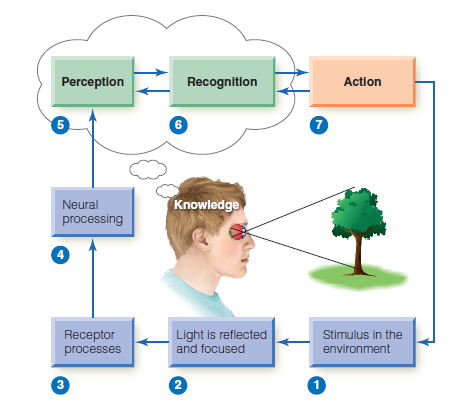
\includegraphics[width=0.75\linewidth,]{images/perceptual-process-goldsein-pg5} 

}

\caption{Perceptual process}\label{fig:perceptual-process}
\end{figure}

When perception occurs, we first experience the \textbf{preattentive stage} in which we observe color, shape, size, and other basic information about the stimuli being perceived. Preattentive perception effects are automatically processed within the first 500 milliseconds of viewing and do not depend on sustained cognitive attention (Vanderplas, Cook, \& Hofmann, 2020).
Following the preattentive stage, \textbf{direct attention} is required for additional processing to allow us to draw connections between components that assist in our interpretation of the stimuli.
When viewing a chart or graph, most insights we gain are due to the cognitive processes that occur after attention is focused on specific aspects of the graph.

The relationship between physiology and perception can provide us information about how graphics may be understood and interpreted.
Through experimentation, the physiological response (automatic reaction) is related to the behavioral response (perception, recognition, and action).
Furmanski \& Engel (2000) tested behavioral responses with functional magnetic resonance imaging (fMRI) techniques to show that the the human visual system is more sensitive to horizontal and vertical stimuli than to stimuli at other orientations.
According to a cognitive analysis, graph interpretation involves (a) relatively simple pattern perception and association processes in which viewers can associate graphic patterns to quantitative referents and (b) more complex and error-prone inferential processes in which viewers must mentally transform data (Shah, Mayer, \& Hegarty, 1999).
Shah \& Carpenter (1995) establish the process in which viewers interact with charts by first perceptually observing the visual features and later translating to cognitive processing of the information depicted by those features.
A viewer must first encode the visual array by identifying meaningful visual features (e.g.~a straight light slanting downward).
Next, the viewer must classify the quantitative measures and relationships in which those visual features illustrate (e.g.~a decreasing linear relationship between x and y).
The last step involves translating the quantitative measures and relationships to the variables defined in the data set (e.g.~a population decreasing over years).
Pyschophysics, the branch of psychology that deals with the relationships between physical stimuli (e.g.~light) and mental phenomena, aims to provide explanations of the relationship between physiology and perception and point out human perceptual biases.
By examining both behavior and physiology together, we are able to understand the mechanisms responsible for perception.

\hypertarget{logarithmic-perception}{%
\subsection{Logarithmic Perception}\label{logarithmic-perception}}

Ernst Weber, an early psychophysics researcher, discovered a phenomenon known as Weber's law, by determining the relationship between the difference threshold (smallest detectable difference between two sensory stimuli; known as the ``Just Noticable Difference'') and the magnitude of a stimulus (Fechner, 1860).
This holds true for a variety of stimuli such as weight, light, and sound as well as for a range of magnitudes; larger numbers require a proportional larger difference in order to remain equally discriminate (Dehaene, Izard, Spelke, \& Pica, 2008).
Known as \textbf{Weber's law}, it was established that we do not notice absolute changes in stimuli, but instead that we notice the relative change (Sun, Wang, Goyal, \& Varshney, 2012).
Numerically, Weber's Law is defined as
\begin{equation}
\frac{\Delta S}{S} = K
\end{equation}
where \(\Delta S\) represents the difference threshold, S represents the initial stimulus intensity, and K is called Weber's contrast which remains constant as the magnitude of S changes.
Gustav Fechner, a founder of psychophysics, provided further extension to Weber's law by discovering the relationship between the perceived intensity is logarithmic to the stimulus intensity when observed above a minimal threshold of perception (Sun, Wang, Goyal, \& Varshney, 2012).
Formally known as the Weber-Fechner law is derived from Weber's law as
\begin{equation}
P = K\ln \frac{S}{S_0}
\end{equation}
where P represents the perceived stimulus, K represents Weber's contrast, S represents the initial stimulus intensity, and \(S_0\) represents the minimal threshold of perception.

\hypertarget{graphical-experiments}{%
\section{Graphical Experiments}\label{graphical-experiments}}

One way in which we determine the relationship between behavior and physiology is through the use of graphical tests (Cleveland \& McGill, 1984; Lewandowsky \& Spence, 1989; Spence, 1990; VanderPlas \& Hofmann, 2015).
These tests may take many forms: identifying differences in graphs, reading information off of a chart accurately, using data to make correct real-world decisions, or predicting the next few observations.
All of these types of tests require different levels of use and manipulation of the information presented in the chart.

The initial push to develop classification and recommendation systems for charts was grounded on heuristics rather than on experimentation (Kruskal, 1975; Macdonald-Ross, 1977).
Request were made for the validation of the perception and utility of statistical charts through graphical experiments.
Initial experiments struggled with methodological issues (Croxton \& Stein, 1932; Croxton \& Stryker, 1927; Eells, 1926) with most early experimentation stemming from psychophysics research on the perception of size and shape (Teghtsoonian, 1965).
Eells (1926) instructed students to think of each circle as representing 100\% and write their best estimate of the percentage of the whole in each sector \pcref{fig:eells-compoment-parts}.
Participants were told not to hurry, but to work steadily in order to determine efficiency of judgment.
Students were then asked to analyze their mental processes used to make their estimates and indicate the method that best matches: by areas of sectors, by central angles, by arcs on the circumference, by subtending chords.
This process was repeated three days later by presenting students the same data represented in bar diagrams.
Results of the study led the authors to argue for the use of circle diagrams to show component parts based on both accuracy and speed.
In response, Croxton \& Stryker (1927) evaluated the accuracy of judgment of two types of charts (bars and circles) in efforts to reach a consistent conclusion.
During class, students were individually presented pairs of diagrams (without scales) on cards and asked to estimate the percentages displayed in the diagram.
It was found that the bar was preferable to the circle when shown percentages that deviate from quarters, but that the circle is strongly preferred when shown percentages separating the diagrams into 25\% or 50\%.

\begin{figure}[tbp]

{\centering 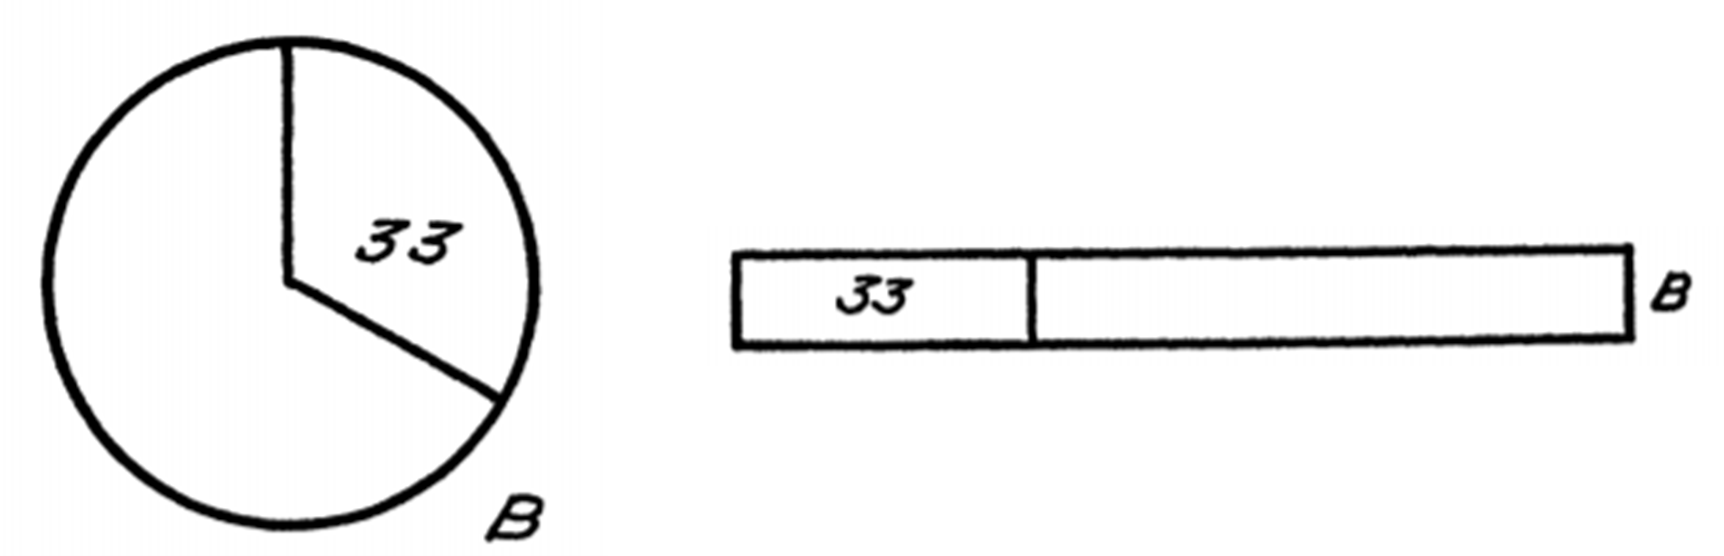
\includegraphics[width=0.75\linewidth,]{images/eells-component-parts} 

}

\caption{Eells (1926) component parts diagrams}\label{fig:eells-compoment-parts}
\end{figure}

While a typical psychophysics experiment focuses on whether an effect is detectable and whether the magnitude of the effect can be accurately estimated, these early experiments instead depended on speed and accuracy for plot evaluation (Lewandowsky \& Spence, 1989; Spence, 1990; Teghtsoonian, 1965).
In Spence (1990), stimuli (tables, lines - horizontal and vertical, bars, boxes, cylinders, pie charts, and disk charts) were presented to participants on a monitor screen in a computer lab.
Participants were asked to use their cursor to position the marker to indicate the proportion to the apparent sizes of the elements \pcref{fig:spence-1990-proportion}.
Results found that the table elements (numbers), pie elements, and bar elements led to the most accurate proportion estimates; boxes and disk elements resulted in the least accurate estimates.
Measuring the speed at which participants made their judgments, it was found that two- and three- dimentional stimuli (e.g.~pie or box) assisted in faster judgment than zero- or one- dimensional stimuli (e.g.~lines).

\begin{figure}[tbp]

{\centering 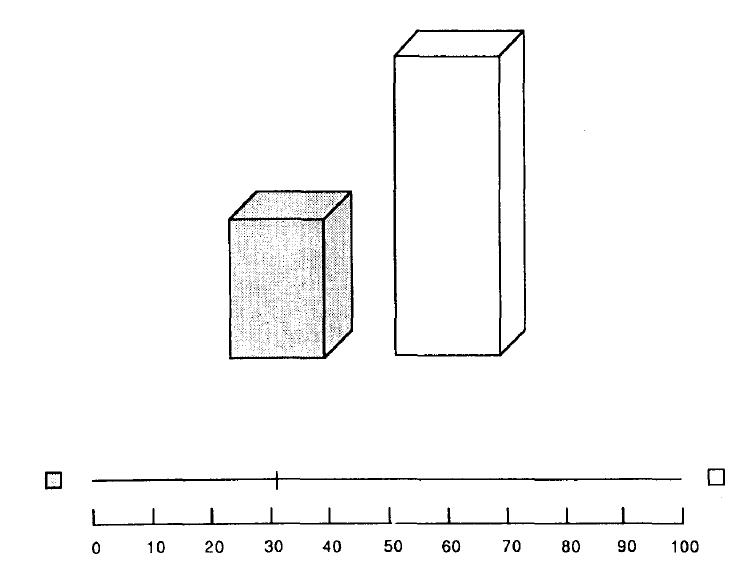
\includegraphics[width=0.75\linewidth,]{images/spence-1990-proportion} 

}

\caption{Spence (1990) task display}\label{fig:spence-1990-proportion}
\end{figure}

Cognitive psychologists and statisticians made progress by conducting experiments to identify perceptual errors associated with different styles of graphics and charts (Cleveland \& McGill, 1984, 1985; Shah, Mayer, \& Hegarty, 1999).
Cleveland \& McGill (1984) provide a basis for perceptual judgment, still utilized today, by examining six basic aesthetic design choices: position along a common scale, position along nonaligned scales, length, angle, slope, and area.
Shah, Mayer, \& Hegarty (1999) established the notion that redesigning graphs can result in the improvement of the viewer's interpretation.
For example, the use of gestalt principles (Goldstein \& Brockmole, 2017) such as proximity, similarity, and good continuation can help minimize the inferential processes and maximize the pattern association processes required to interpret relevant information.

These later experiments followed similar methodology as early studies by asking participants to read information directly from the charts and provide a quantitative estimate or answer a predefined question; as with the early studies, accuracy and response time were evaluated (Amer, 2005; Broersma \& Molenaar, 1985; Dunn, 1988; L. V. Peterson \& Schramm, 1954; Tan, 1994).
\svp{relate these examples to their implications - i.e. quantitative translation}
Spence (1990) presents four example questions for comparing the sizes of individual graphical elements: (1) How much greater was the rainfall in September than May? (2) Is the price of oil in constant dollars increasing or decreasing from year to year? (3) Do more people subscribe to Time than Newsweek? and (4) Did the ABC Corporation pay the largest dividends last year, or did XYZ?
Amer (2005) demonstrates that visual illusion may bias decision making and graph comprehension, even if the graphs are constructed according to best practice.
Participants were presented a cost volume profit graph \pcref{fig:amer-poggendorff-illusion} with two crossing lines (revenue and cost) and asked to view three values: (1) the amount of total revenues on the ordinate corresponding to the endpoint of the total-revenue line plotted on the graph (2) the amount of total costs on the ordinate corresponding to the endpoint of the total-cost line plotted on the graph and (3) the amount of costs/revenues on the ordinate at the break even point---the point where the two lines cross.
Results indicate that decision makers may consistentily underestimate or overestimate the values displayed on line graphs due to what is called the ``Poggendorff illusion.''
In Dunn (1988), participants were shown two maps, an unclassed choropleth map and a framed rectrangle chart, indicating the murder rate of each US state \pcref{fig:framed-murder-rate-map}.
The goal of the study was to assess the relative accuracy with which quantitative information is extracted from both types of charts.
Participants were strictly informed that the experiment was designed to test the ability of individuals to ``read'' or ``decode'' statistical maps and asked to write down their estimate of the murder rate as accurately as possible beside the 24 named states.
Results indicate that subjects found it easier to extract quantitative information from the framed rectangle chart than from the unclassed choropleth map and that the between individual variability in the choropleth map was related to the area of the state.

\begin{figure}[tbp]

{\centering 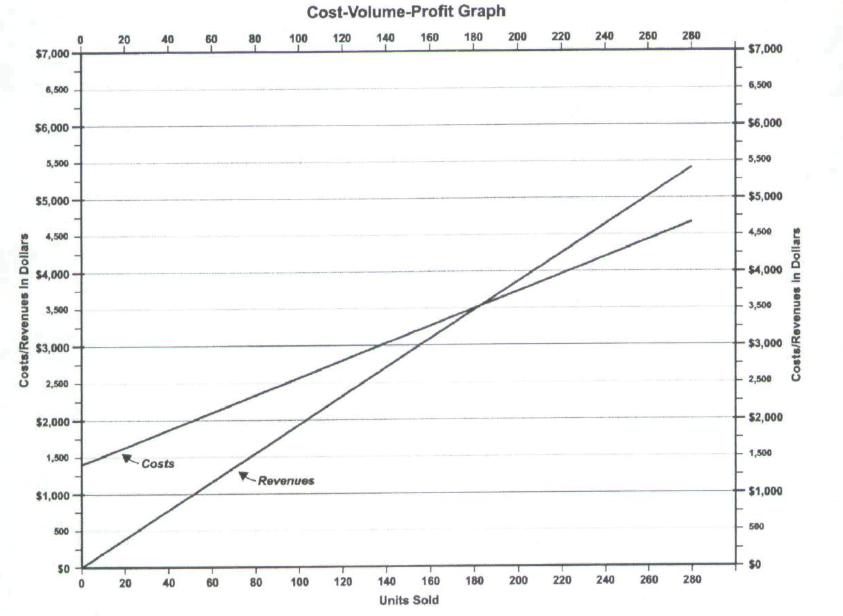
\includegraphics[width=0.9\linewidth,]{images/amer-poggendorff-illusion} 

}

\caption{Amer (2005) cost volume profit graph}\label{fig:amer-poggendorff-illusion}
\end{figure}

\begin{figure}[tbp]

{\centering 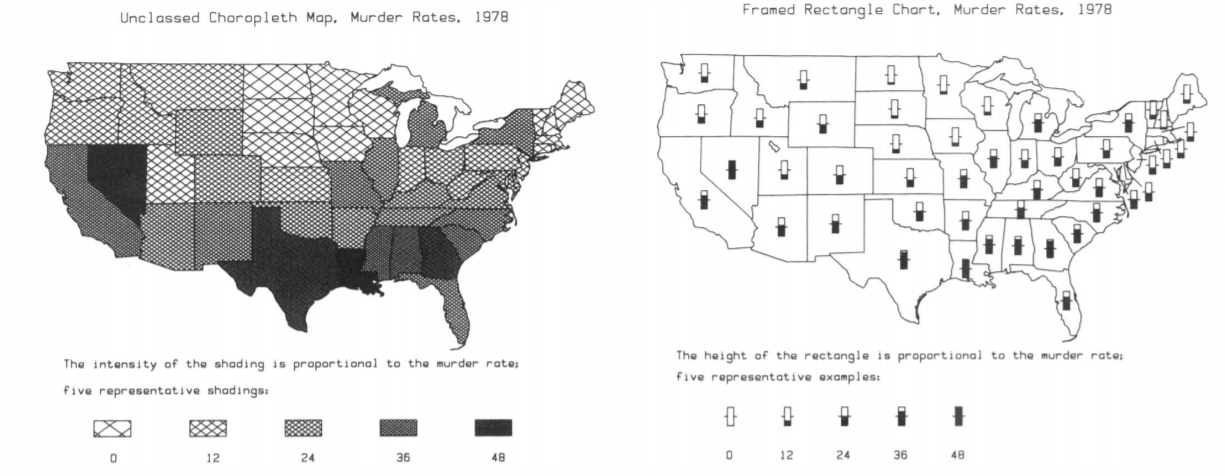
\includegraphics[width=0.9\linewidth,]{images/framed-murder-rate-map} 

}

\caption{Dunn (1988) maps}\label{fig:framed-murder-rate-map}
\end{figure}

During the \(\text{21}^{\text{st}}\) century, there have been advancements in the methodology used to investigate the effectiveness of statistical charts (Majumder, Hofmann, \& Cook, 2013).
Buja et al. (2009) introduced the lineup protocol in which data plots are depicted and interpreted as statistics.
Supported by the grammar of graphics, a data plot can be characterized as a statistic defined as, ``a functional mapping of a variable or set of variables'' (Vanderplas, Cook, \& Hofmann, 2020).
This allows the data plot to be tested similar to other statistics, by comparing the actual data plot to a set of plots with the absence of any data structure we can test the likelihood of any perceived structure being significant.
The construction of data plots as statistics allow for easy experimentation, granting researchers the ability to compare the effectiveness of and understand the perception of different types of charts.
While the lineup protocol differs from methodology used in earlier studies, the focus is still on initial perception and graph comprehension with a relatively small amount of work conducted to understand the effect of design choices on higher cognitive processes such as learning or analysis (Green \& Fisher, 2009).
Lineups serve as a powerful tool for testing \emph{perceived} differences by eliminated ambiguous questions.
However, the lineup protocol is constrained by the inability to test higher order cognitive skills such as accurately reading information off of a graph or drawing conclusions from the graph; limiting their ability to be used for testing real-world applications.

\hypertarget{logarithmic-scales-and-mapping}{%
\section{Logarithmic Scales and Mapping}\label{logarithmic-scales-and-mapping}}

We have recently experienced the impact graphics and charts have on a large scale through the SARSNCOV-2 pandemic (COVID-19).
At the beginning of 2020, we saw an influx of dashboards being developed to display case counts, transmission rates, and outbreak regions (Rost, 2020); mass media routinely showed charts to share information with the public about the progression of the pandemic (Romano, Sotis, Dominioni, \& Guidi, 2020).
Fagen-Ulmschneider (2020) began the 91-DIVOC project to explore the global growth of COVID-19 through interactive graphics updated daily.
The interactive graphics allowed viewers to explore the current status of COVID-19 by selecting their desired regions, axes, axis scale, and measure of interest (e.g.~case count, death count, vaccine count); \cref{fig:91divoc-cases-july2021} shows the new confirmed COVID-19 cases per day, normalized by population, as of July 2021.
Other graphics displayed COVID-19 data as maps \pcref{fig:covid19-summer2020-risk-map} with color indicating the severity and risk in each US county ({``Risk levels,''} 2021).
People began seeking out graphical displays of COVID-19 data as a direct result of these pieces of work (Rost, 2020); providing increased and ongoing exposure to these graphics over time.
\cref{fig:covid19-datawrapper-views-july2020} illustrates the increased views Datawrapper, a user-friendly web tool used to create basic interactive charts, had during the COVID-19 pandemic (Rost, 2020).
Many of these graphics helped guide decision makers to implement policies such as shut-downs or mandated mask wearing, as well as facilitated communication with the public to increase compliance (Bavel et al., 2020).
As graphics began to play an important role in the communication of the pandemic, creators of graphics were faced with design choices in order to ensure their charts were effective.

\begin{figure}[tbp]

{\centering 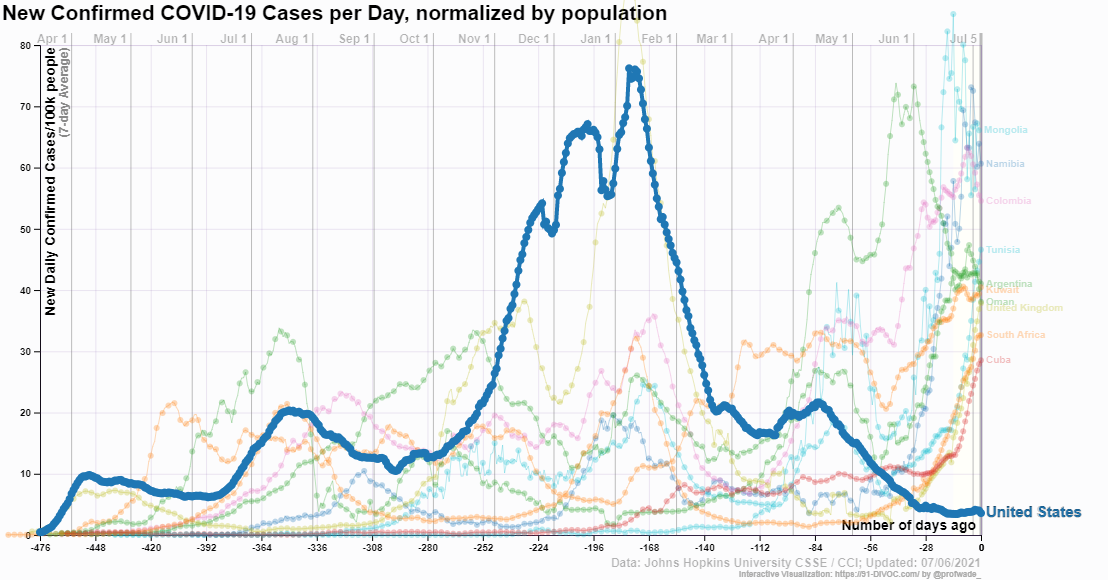
\includegraphics[width=0.9\linewidth,]{images/91dovic-cases-july2021} 

}

\caption{91-DOVIC New Daily Case Counts as of July 2021}\label{fig:91divoc-cases-july2021}
\end{figure}

\begin{figure}[tbp]

{\centering 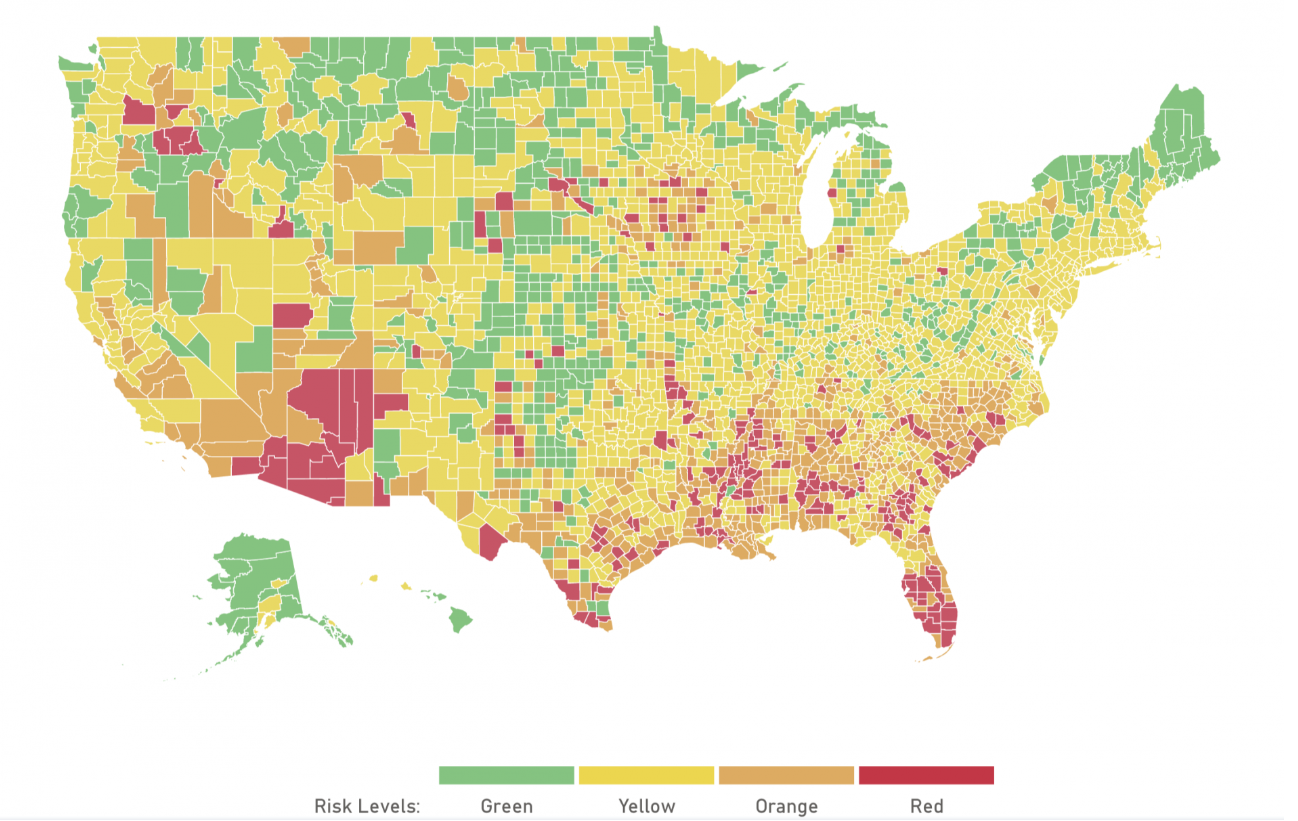
\includegraphics[width=0.9\linewidth,]{images/covid19-summer2020-risk-map} 

}

\caption{COVID-19 Risk Level Map as of July 2020}\label{fig:covid19-summer2020-risk-map}
\end{figure}

\begin{figure}[tbp]

{\centering 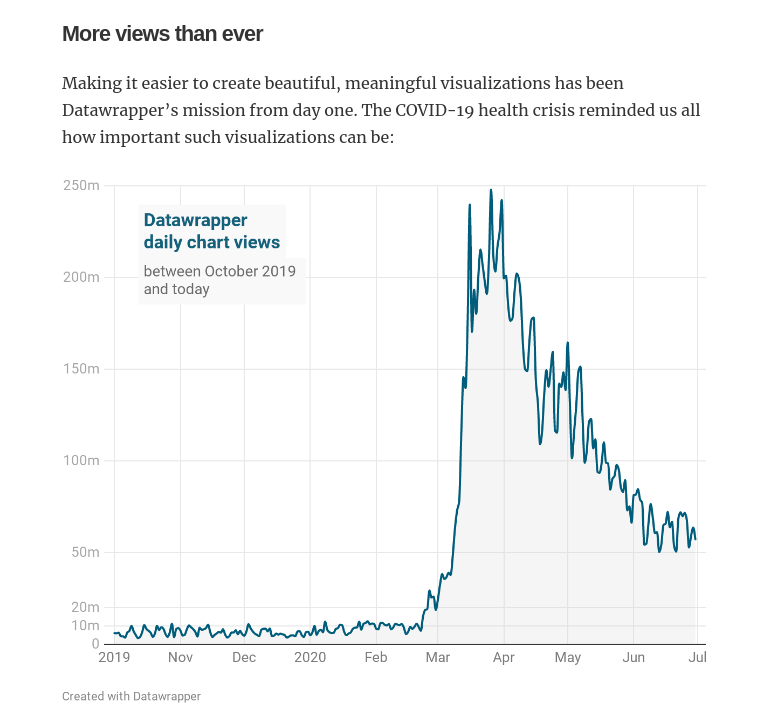
\includegraphics[width=0.9\linewidth,]{images/covid19-datawrapper-views-july2020} 

}

\caption{Datawrapper daily chart views during COVID-19}\label{fig:covid19-datawrapper-views-july2020}
\end{figure}

When faced with data which spans several orders of magnitude, we must decide whether to show the data on its original
scale (compressing the smaller magnitudes into relatively little area) or to transform the scale and alter the contextual appearance of the data.
The usefulness of the log scale in science is illustrated in \cref{fig:log-scale-comic} (Munroe, 2005) showing the challenge of displaying the fuel energy density of Uranium along side other sources of fuel due to differences in magnitude.
One common solution is to use a log scale transformation to display data over several orders of magnitude within one graph.
\cref{fig:log-scales} presents an exponential curve displayed on both the linear and log scale illustrating the use of the log scale when displaying data which spans several magnitudes.
Logarithms convert multiplicative relationships (for example, 1 \& 10 displayed 10 units apart and 10 \& 100 displayed 90 units apart) to additive relationships (for example, 1 \& 10 and 10 \& 100 both equally spaced along the axis), showing proportional relationships and linearizing power functions (Menge et al., 2018).
They also have practical purposes, easing the computation of small numbers such as likelihoods and transforming data to fit statistical assumptions.
When presenting log scaled data, it is possible to use either un-transformed scale labels (for example, values of 1, 10 and 100 are equally spaced along the axis) or log transformed scale labels (for example, 0, 1, and 2, showing the corresponding powers of 10).

\begin{figure}[tbp]

{\centering 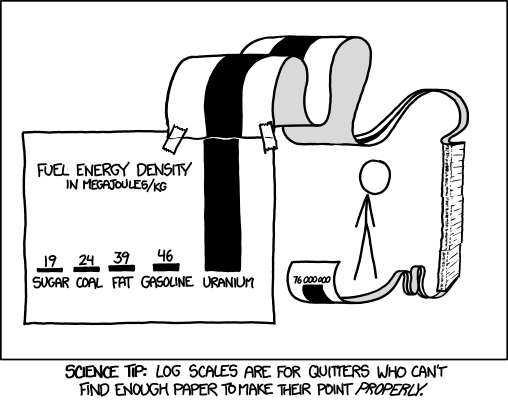
\includegraphics[width=0.7\linewidth,]{images/log-scale-comic} 

}

\caption{Usefulness of the log scale in science}\label{fig:log-scale-comic}
\end{figure}

\begin{figure}[tbp]

{\centering 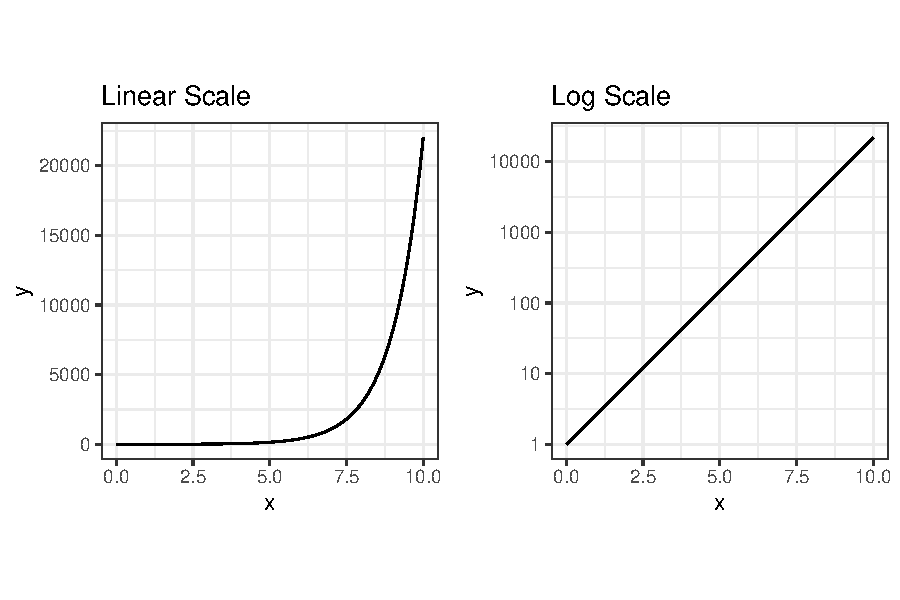
\includegraphics[width=1\linewidth,]{thesis_files/figure-latex/log-scales-1} 

}

\caption{Linear scale verses log scale}\label{fig:log-scales}
\end{figure}

We have recently experienced the benefits and pitfalls of using log scales as COVID-19 dashboards displayed
case count data on both the log and linear scale (Burn-Murdoch et al., 2020; Fagen-Ulmschneider, 2020).
In spring 2020, during the early stages of the COVID-19 pandemic, there were large magnitude discrepancies in case counts at a given time point between different geographic regions (e.g.~states and provinces as well as countries and continents).
During this time, we saw the usefulness of log scale transformations showing case count curves for areas with few cases and areas with many cases within one chart.
\cref{fig:covid19-FT-deaths-march2020-log} illustrates the usefulness of log scales in comparing deaths attributed to Coronavirus between countries as of March 2020; the diagonal reference lines provide a visual aid useful for interpretation (Burn-Murdoch et al., 2020).
As the pandemic evolved, and the case counts were no longer spreading exponentially, graphs with linear scales seemed more effective at spotting early increases in case counts that signaled more localized outbreaks. In \cref{fig:covid19-FT-june2020-case-counts-linear} and \cref{fig:covid19-FT-june2020-case-counts-log}, the case counts as of June 30, 2020 are displayed on both the linear and log scale respectively (Burn-Murdoch et al., 2020).
The effect of the linear scale \pcref{fig:covid19-FT-june2020-case-counts-linear} appears to evoke a stronger reaction from the public than the log scale \pcref{fig:covid19-FT-june2020-case-counts-log} as case counts are clearly rising rapidly during the summer wave.
This is only one recent example of a situation in which both log and linear scales are useful for showing different aspects of the same data.
There are long histories of using log scales to display results in ecology, psychophysics, engineering, and physics (Heckler, Mikula, \& Rosenblatt, 2013; Menge et al., 2018)
In Waddell (2005), comparisons were made between the linear and logarithmic scales for dosage verses carcinogenicity in rodents.
Results favored the use of logarithmic scales for doses in order to put the relative doses into perspective whereas using a linear scale to administer doses to animals with doses of those same chemicals to which humans are exposed does not provide useful, comparative information.
Given the widespread use of logarithmic scales, it is important to understand the implications of their use in order to provide guidelines for best use.

\begin{figure}[tbp]

{\centering 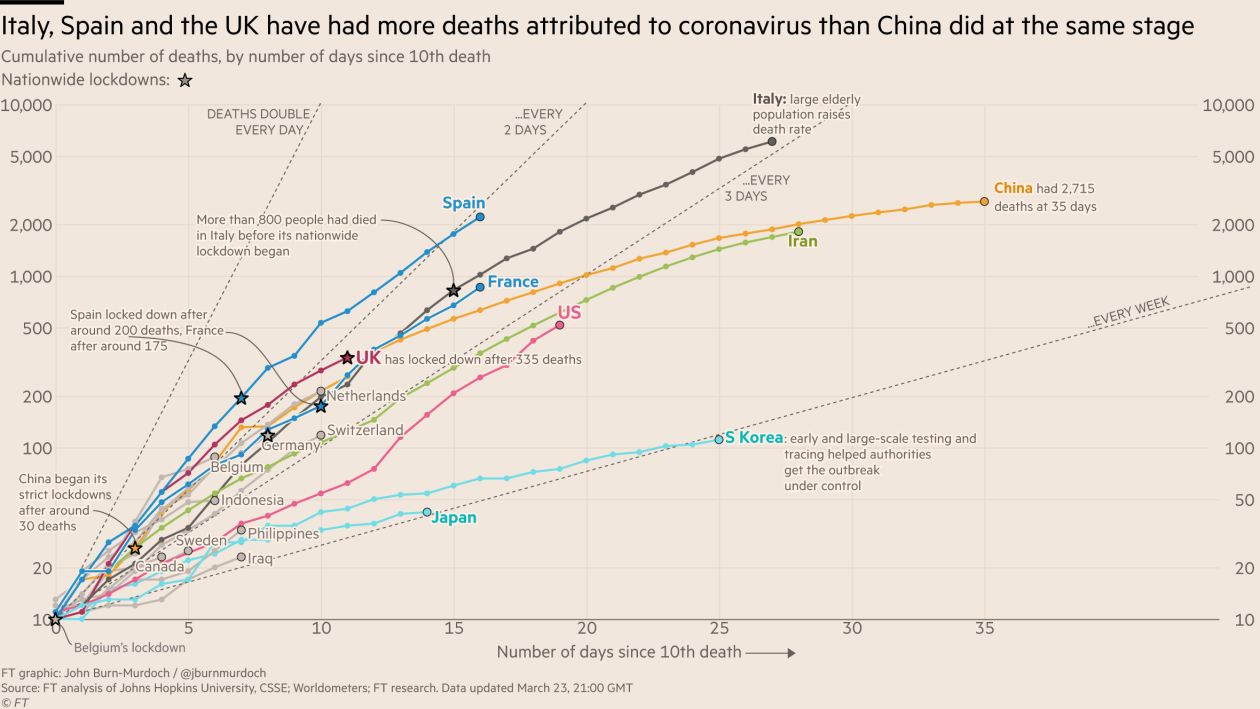
\includegraphics[width=0.9\linewidth,]{images/covid19-FT-03.23.2020-log} 

}

\caption{Covid 19 Deaths (log scale) as of March 23, 2020}\label{fig:covid19-FT-deaths-march2020-log}
\end{figure}

\begin{figure}[tbp]

{\centering 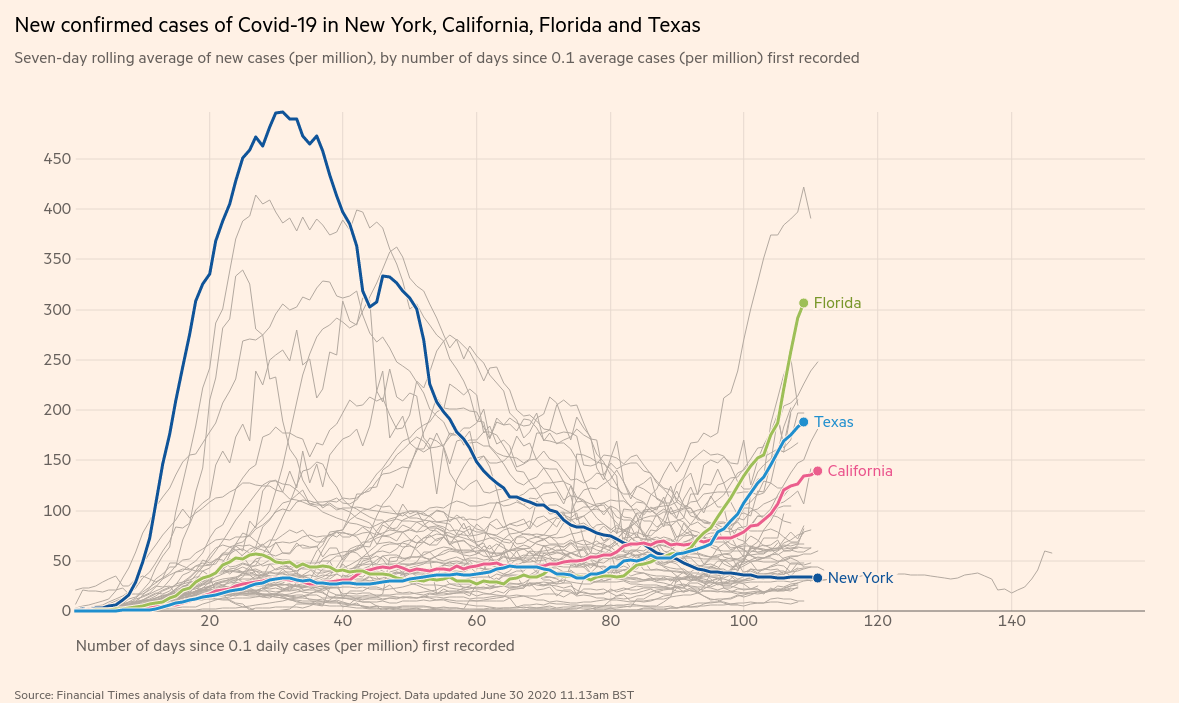
\includegraphics[width=0.9\linewidth,]{images/covid19-FT-case-count-06.30.2020-linear} 

}

\caption{Covid 19 Case Counts (linear scale) as of June 30, 2020}\label{fig:covid19-FT-june2020-case-counts-linear}
\end{figure}

\begin{figure}[tbp]

{\centering 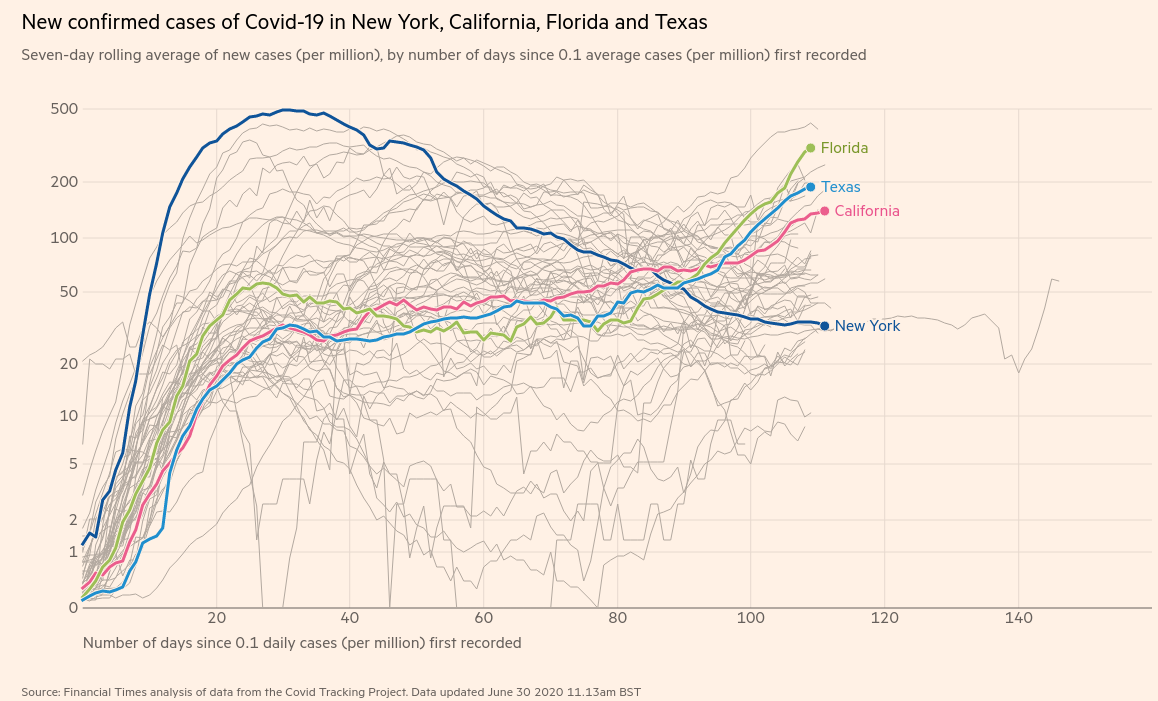
\includegraphics[width=0.9\linewidth,]{images/covid19-FT-case-count-06.30.2020-log} 

}

\caption{Covid 19 Case Counts (log scale) as of June 30, 2020}\label{fig:covid19-FT-june2020-case-counts-log}
\end{figure}

When we first learn to count, we begin counting by ones (for example, 1, 2, 3, etc.), then by tens (for example, 10, 20, 30, etc.), and advancing to hundreds (for example, 100, 200, 300, etc.), following the base10 order of magnitude system (for example, 1, 10, 100, etc.).
Research suggests our perception and mapping of numbers to a number line is logarithmic at first, but transitions to a linear scale later in development, with formal mathematics education (Dehaene, Izard, Spelke, \& Pica, 2008; Siegler \& Braithwaite, 2017, 2017; Varshney \& Sun, 2013).
For example, a kindergartner asked to place numbers 1-10 along a number line would place 3 close to the middle, following the logarithmic perspective (Varshney \& Sun, 2013); \cref{fig:log-number-line} demonstrates how a kindergartner might map numbers along a number line.
Dehaene, Izard, Spelke, \& Pica (2008) found that with basic training, members of remote cultures with a basic vocabulary and minimal education understood the concept that numbers can be mapped into a spacial space; for example, numbers can be mapped to a number line or numbers can be mapped onto a clock.
There was a gradual transition from logarithmic to linear scale as the mapping of whole number magnitude representations transitioned from a compressed (approximately logarithmic) distribution to an approximately linear one.
These results indicate the universal and cultural-dependent characteristics of the sense of number.

\begin{figure}[tbp]

{\centering 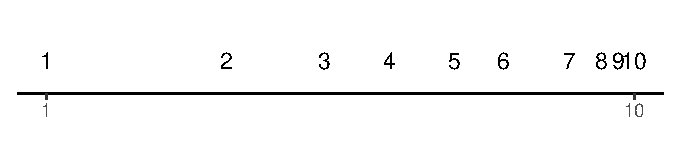
\includegraphics[width=\linewidth,]{thesis_files/figure-latex/log-number-line-1} 

}

\caption{Kindergarten example of mapping numbers 1-10 along a number line}\label{fig:log-number-line}
\end{figure}

Assuming there is a direct relationship between perceptual and cognitive processes, it is reasonable to assume numerical representations should also be displayed on a nonlinear, compressed number scale. Therefore, if we perceive logarithmically by default, it is a natural (and presumably low effort) way to display information and should be easy to read and understand/use.
The idea is compression enlarges the coding space, thus increasing the dynamic range of perception and firing neurons within our visual system (Nieder \& Miller, 2003).
Similar to the training and education required to transition from logarithmic mapping to linear mapping, there is also necessary training required in the assessment of graphical displays associated with logarithmic scales. Haemer \& Kelley (1949) identify semi-logarithmic charts for temporal series as requiring a certain degree of technical training.

\hypertarget{underestimation}{%
\section{Underestimation of Exponential Growth}\label{underestimation}}

The same data can be interpreted differently by people with differing backgrounds; \cref{fig:exponential-stages-comic} (Bergmann, 2021) illustrates how exponential growth is interpreted by individuals in public health vastly different than scientists.
Exponential growth is often misjudged in early stages appearing to have a small growth rate.
As exponential growth continues, the middle stage appears to be growing, but not at an astounding rate, appearing more quadratic.
It is not until late stages of exponential growth when it is quite apparent that there is exponential growth occurring.
This can lead to decisions made under inaccurate understanding causing future consequences.
Early studies explored the estimation and prediction of exponential growth and found that growth is underestimated when presented both numerically and graphically (Wagenaar \& Sagaria, 1975).
Results indicated that numerical estimation is more accurate than graphical estimation for exponential curves,
Experimental studies were conducted in order to determine strategies to improve estimation of exponential growth (Jones, 1977; Mackinnon \& Wearing, 1991; Wagenaar \& Sagaria, 1975)
There was no improvement in estimation found when participants had contextual knowledge or experience with exponential growth, but instruction on exponential growth reduced the underestimation; participants adjusted their initial starting value but not their perception of the growth rate (Jones, 1977; Wagenaar \& Sagaria, 1975).
Mackinnon \& Wearing (1991) found that estimation was improved by providing immediate feedback to participants about the accuracy of their current predictions.\\
Our inability to accurately predict exponential growth might also be addressed by log transforming the data, however, this transformation introduces new complexities; most readers are not mathematically sophisticated enough to intuitively understand logarithmic math and translate that back into real-world effects.

\begin{figure}[tbp]

{\centering 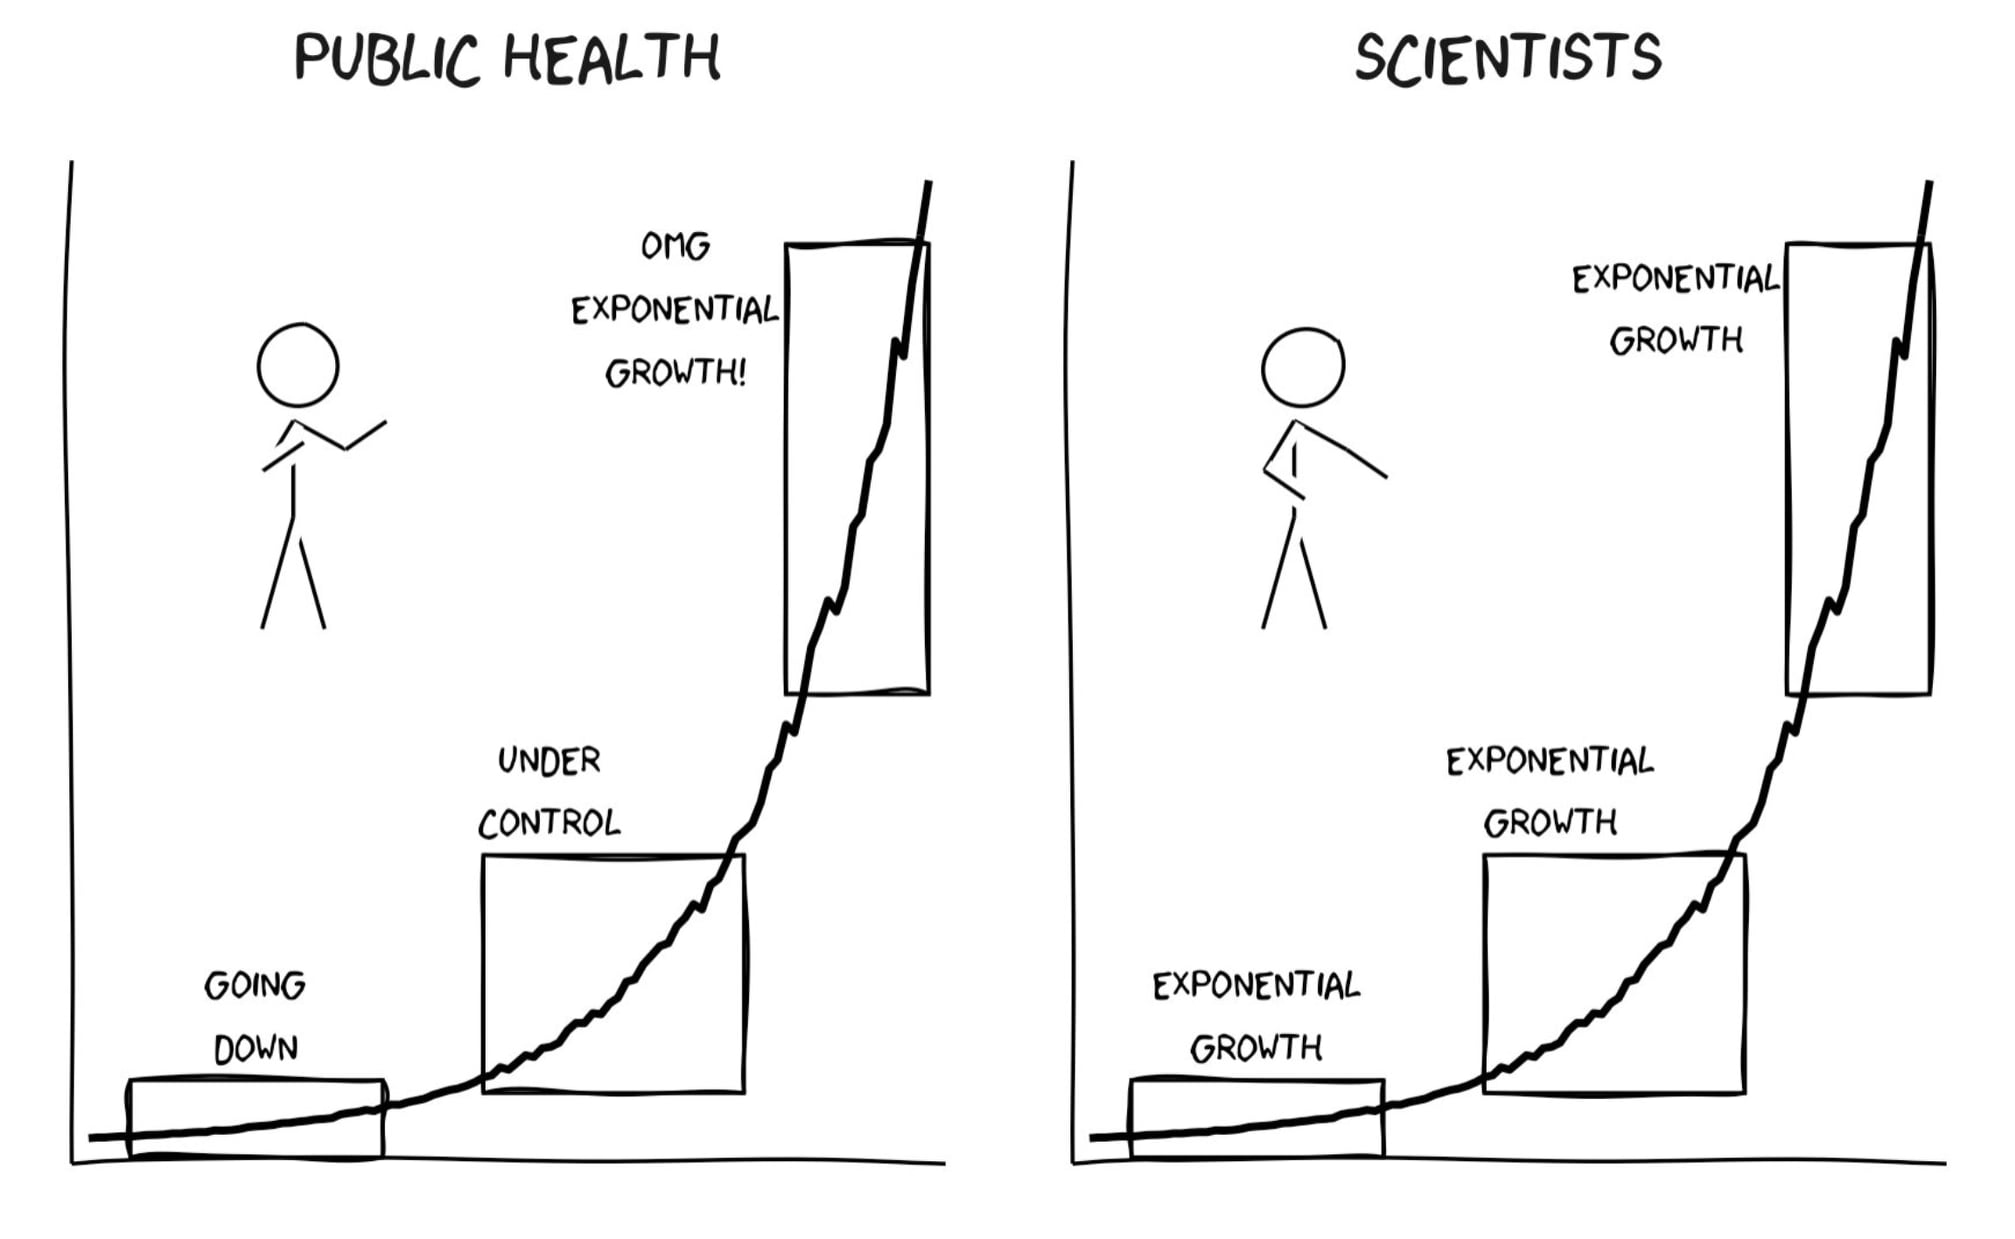
\includegraphics[width=1\linewidth,]{images/exponential-stages-comic} 

}

\caption{Log scale comic}\label{fig:exponential-stages-comic}
\end{figure}

In Menge et al. (2018), ecologists were surveyed to determine how often ecologists encounter log scaled data and how well ecologists understand log scaled data when they see it in the literature.
Participants were presented three relationships displayed on linear-linear scales, log-log scales with untransformed values, or log--log scales with log transformed values \pcref{fig:menge-plots}.
The authors propose three types of misconceptions participants encountered when presented data on log-log scales: `hand-hold fallacy,' `Zeno's zero fallacy,' and `watch out for curves fallacies.'
These misconceptions are a result of linear extrapolation assuming that a line in log-log space represents a line instead of the power law in linear-linear space.
The study found that in each of these scenarios, participants were confident in their incorrect responses, indicating incorrect knowledge rather than a lack of knowledge.

\begin{figure}[tbp]

{\centering 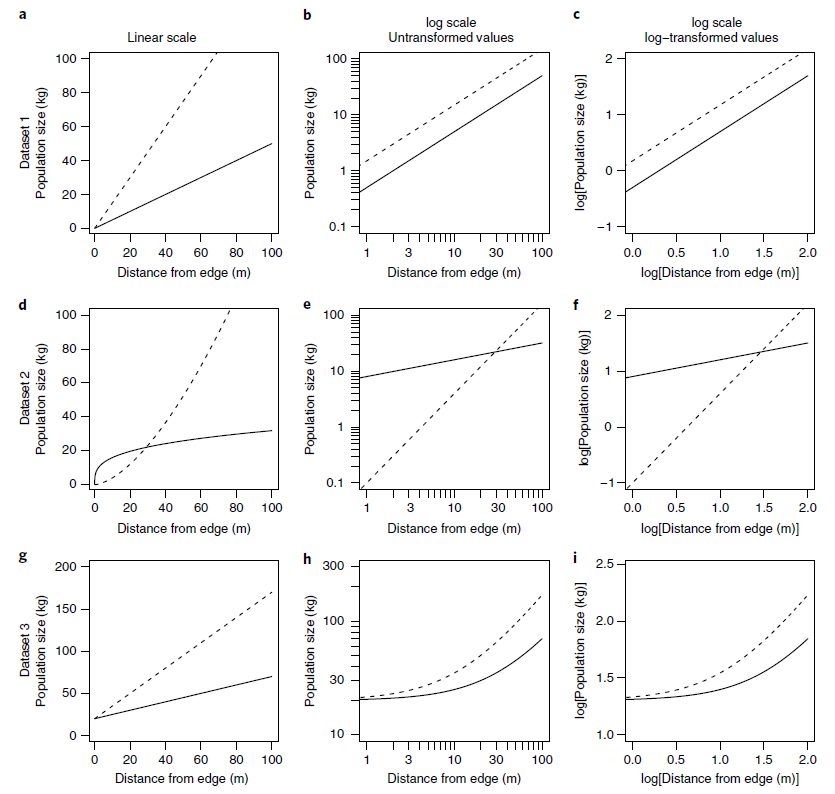
\includegraphics[width=0.75\linewidth,]{images/menge-plots} 

}

\caption{Graphs viewed in Menge (2018) survey}\label{fig:menge-plots}
\end{figure}

The `hand-hold fallacy' stems from the misconception that steeper slopes in log-log relationships are steeper slopes in linear-linear space, illustrated in \cref{fig:menge-plots} d-f.~
In fact, it is not only the slope that matters, but also the intercept and the location on the horizontal axis since a line in log-log space represents a power law in linear-linear space (i.e.~linear extrapolation).
Emerging from `Zeno's zero fallacy' is the misconception that positively sloped lines in log-log space can imply a non-zero value of y when x is zero, illustrated in \cref{fig:menge-plots} a-c and d-f.
This is never true as positively sloped lines in log-log space actually imply that y = 0 when x = 0. This misconception again is a result of linear extrapolation assuming that a line in log-log space represents a line instead of the power law in linear-linear space.
The last misconception, `watch out for curves fallacies' encompasses three faults: (1) lines in log-log space are lines in linear-linear space (illustrated in \cref{fig:menge-plots} d-f), (2) lines in log-log space curve upward in linear-linear space (illustrated in \cref{fig:menge-plots} d-f), and (3) curves in log-log space have the same curvature in linear-linear space (illustrated in \cref{fig:menge-plots} g-i).
Linear extrapolation is again responsible for the first and third faults while the second fault is a result of error in thinking that log-log lines represent power laws (which are exponential relationships), and all exponential relationships curve upward; this is only true when the log-log slope is greater than 1.
Menge et al. (2018) found that in each of these scenarios, participants were confident in their incorrect responses, indicating incorrect knowledge rather than a lack of knowledge.

\hypertarget{research-objectives}{%
\section{Research Objectives}\label{research-objectives}}

In my research, I conduct three graphical experimental tasks to evaluate the impact our choice of scale (log/linear) has on human perception of exponentially increasing trends.
The first experiment evaluates whether our ability to perceptually notice differences in exponentially increasing trends is impacted by the choice of scale. I conducted a visual inference experiment in which participants were shown a series of lineup plots and asked to identify the panel that was most different from the others.
The other experimental tasks focus on determining whether there are cognitive disadvantages to log scales: do log scales make it harder to make use of graphical information?
I conducted a graphical task similar to the New York Times ``You Draw It'' page to test an individual's ability to use and make predictions for exponentially increasing data.
Participants were asked to draw a line using their computer mouse through the increasing exponential trend shown on both scales.
In addition to differentiation and prediction of exponentially increasing data, an experimental task was conducted to test an individuals' ability to translate a graph of exponentially increasing data into real value quantities and extend their estimations by making comparisons.
The results of the three experimental tasks provide guidelines for readers to actively choose which of many possible graphics to draw, according to some set of design choices, to ensure that their charts are effective.

\hypertarget{lineups}{%
\chapter{Perception through lineups}\label{lineups}}

\hypertarget{introduction}{%
\section{Introduction}\label{introduction}}

Previously, we saw how a data plot can be evaluated and treated as a visual statistic, a numerical function which summarizes the data.
To evaluate a graph, we have to run our statistic through a visual evaluation - a person.
If two different methods of presenting data result in qualitatively different results when evaluated visually, then we can conclude that the visual statistics are significantly different.
Recent graphical experiments have utilized statistical lineups to quantify the perception of graphical design choices (Hofmann, Follett, Majumder, \& Cook, 2012; Loy, Follett, \& Hofmann, 2016; Loy, Hofmann, \& Cook, 2017; VanderPlas \& Hofmann, 2017).
Statistical lineups provide an elegant way of combining perception and statistical hypothesis testing using graphical experiments (Majumder, Hofmann, \& Cook, 2013; Vanderplas, Cook, \& Hofmann, 2020; H. Wickham, Cook, Hofmann, \& Buja, 2010).
`Lineups' are named after the `police lineup' of criminal investigations where witnesses are asked to identify the criminal from a set of individuals.
Similarly, a statistical lineup is a plot consisting of smaller panels; the viewer is asked to identify the plot of the real data from among a set of decoy null plots.
Null plots display data under the assumption there is no relationship and can be generated by permutation or simulation.
A statistical lineup typically consists of 20 panels - 1 target panel and 19 null panels.
If the viewer can identify the target panel embedded within the set of null panels, this suggests that the real data is visually distinct from data generated under the null model.
\cref{fig:lineup-example} provides example's of a statistical lineup's.
The lineup plot on the left displays increasing exponential data on a linear scale with panel (2 x 5) + 3 as the target.
The lineup plot on the right displays increasing exponential data on the log scale with panel 2 x 2 as the
target.
Crowd sourcing websites such as Amazon Mechanical Turk, Reddit, and Prolifc allow us to collect responses from multiple viewers.

\begin{figure}[tbp]

{\centering 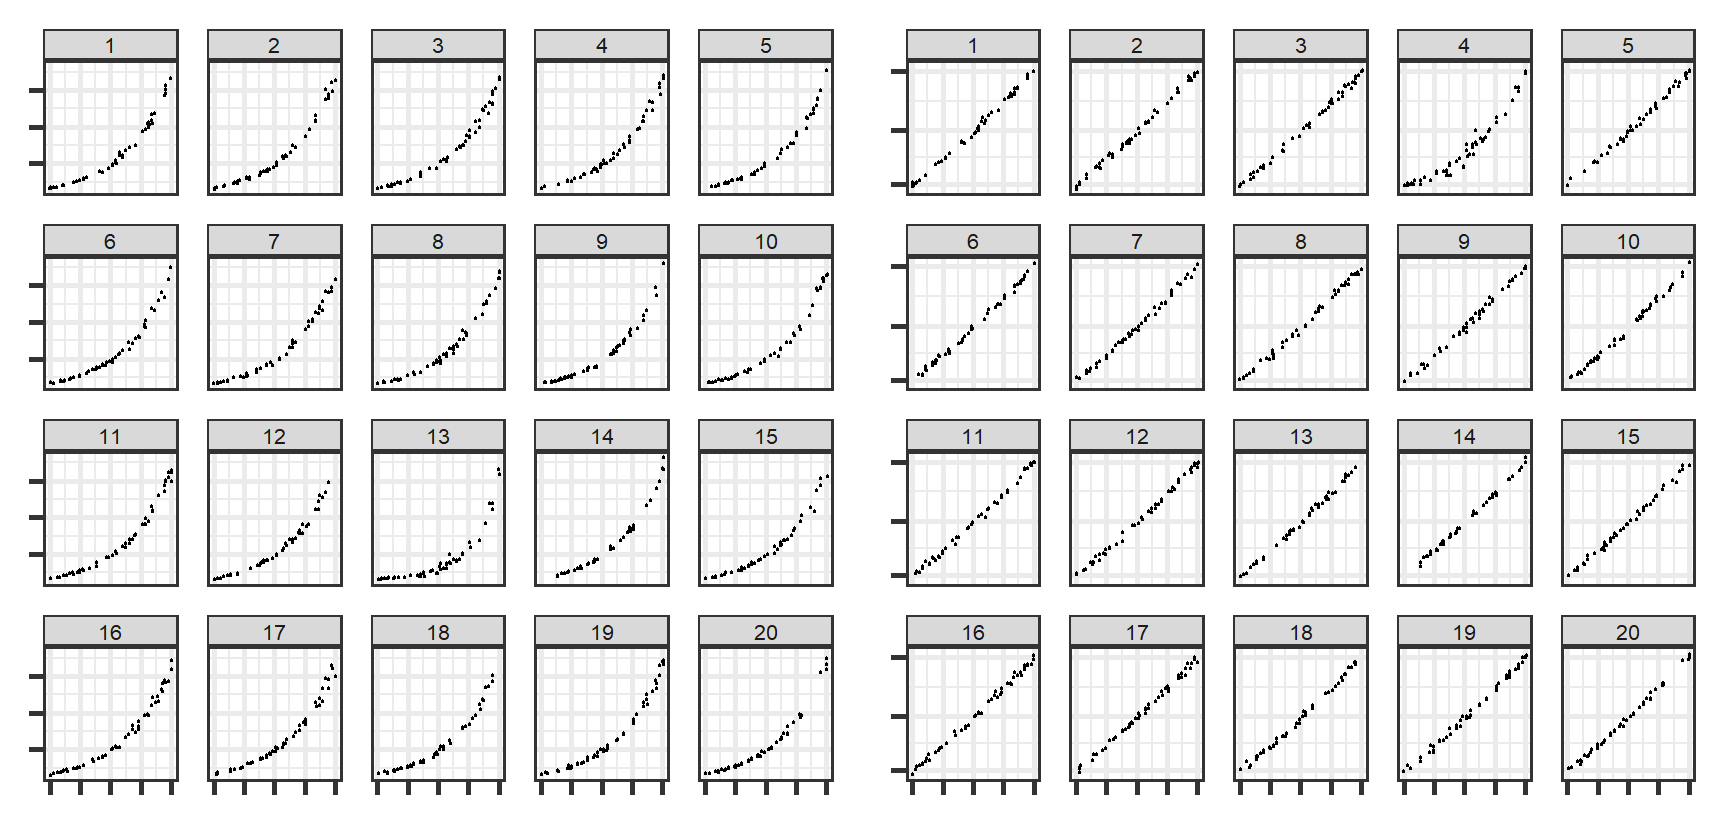
\includegraphics[width=\linewidth,]{thesis_files/figure-latex/lineup-example-1} 

}

\caption{Example Lineups}\label{fig:lineup-example}
\end{figure}

While explicit graphical tests direct the participant to a specific feature of a plot to answer a specific question, implicit graphical tests require the user to identify both the purpose and function of the plot in order to evaluate the plots shown (Vanderplas, Cook, \& Hofmann, 2020).
Implicit graphical tests, such as lineups, have the advantage of simultaneously visually testing for multiple visual features including outliers, clusters, linear and nonlinear relationships.
To lay a foundation for future exploration of the use of log scales, we begin with the most fundamental ability to identify differences in charts; this does not require that participants understand exponential growth, identify log scales, or have any mathematical training.
Instead, we are simply testing the change in perceptual sensitivity resulting from visualization choices.
The study in this chapter is conducted through visual inference and the use of statistical lineups to differentiate between exponentially increasing curves with differing levels of curvature, using linear and log scales.

\hypertarget{data-generation}{%
\section{Data Generation}\label{data-generation}}

In this study, both the target and null data sets were generated by simulating data from an exponential model; the models differ in the parameters selected for the null and target panels.
In order to guarantee the simulated data spans the same domain and range of values, we implemented a domain constraint of \(x\in [0,20]\) and a range constraint of \(y\in [10,100]\) with \(N = 50\) points randomly assigned throughout the domain and mapped to the y-axis using the exponential model with the selected parameters.
These constraints provide some assurance that participants who select the target plot are doing so because of their visual perception differentiating between curvature or growth rate rather than different starting or ending values.

Data was simulated based on a three-parameter exponential model with multiplicative errors:
\begin{align}
y_i & = \alpha\cdot e^{\beta\cdot x_i + \epsilon_i} + \theta \\
\text{with } \epsilon_i & \sim N(0, \sigma^2). \nonumber
\end{align}
The parameters \(\alpha\) and \(\theta\) are adjusted based on \(\beta\) and \(\sigma^2\) to guarantee the range and domain constraints are met.
The model generated \(N = 50\) points \((x_i, y_i), i = 1,...,N\) where \(x\) and \(y\) have an increasing exponential relationship.
The heuristic data generation procedure is described below:

\begin{algorithm}
  \caption{Lineup Parameter Estimation}
  \begin{algorithmic}[1]
    \Statex \textbullet~\textbf{Input Parameters:} domain $x\in[0,20]$, range $y\in[10,100]$, midpoint $x_{mid}$.
    \Statex \textbullet~\textbf{Output Parameters:} estimated model parameters $\hat\alpha, \hat\beta, \hat\theta$.
    \State Determine the $y=-x$ line scaled to fit the assigned domain and range.
    \State Map the values $x_{mid} - 0.1$ and $x_{mid} + 0.1$ to the $y=-x$ line for two additional points.
    \State From the set points $(x_k, y_k)$ for $k = 1,2,3,4$, obtain the coefficients from the linear model $\ln(y_k) = b_0 +b_1x_k$ to obtain starting values - $\alpha_0 = e^{b_0}, \beta_0 =  b_1, \theta_0 = 0.5\cdot \min(y)$
    \State Using the `nls()` function from the `stats` package in Rstudio and the starting parameter values - $\alpha_0, \beta_0, \theta_0$ - fit the nonlinear model, $y_k = \alpha\cdot e^{\beta\cdot x_k}+\theta$ to obtain estimated parameter values - $\hat\alpha, \hat\beta, \hat\theta.$
  \end{algorithmic}
\end{algorithm}

\begin{algorithm}
  \caption{Lineup Exponential Data Simulation}
  \begin{algorithmic}[1]
    \Statex \textbullet~\textbf{Input Parameters:} sample size $N = 50$, estimated parameters $\hat\alpha$, $\hat\beta$, and $\hat\theta$, $\sigma$ standard deviation from the exponential curve.
    \Statex \textbullet~\textbf{Output Parameters:} $N$ points, in the form of vectors $\mathbf{x}$ and $\mathbf{y}$.
    \State Generate $\tilde x_j, j = 1,..., N\cdot \frac{3}{4}$ as a sequence of evenly spaced points in $[0,20]$. This ensures the full domain of $x$ is used, fulfilling the constraints of spanning the same domain and range for each parameter combination.
    \State Obtain $\tilde x_i, i = 1,...N$ by sampling $N = 50$ values from the set of $\tilde x_j$ values. This gaurantees some variability and potential clustring in the exponential growth curve disrupting the perception due to continuity of points.
    \State Obtain the final $x_i$ values by jittering $\tilde x_i$.
    \State Calculate $\tilde\alpha = \frac{\hat\alpha}{e^{\sigma^2/2}}.$ This ensures that the range of simulated values for different standard devaition parameters has an equal expected value for a given rate of change due to the non-constant variance across the domain.
    \State Generate $y_i = \tilde\alpha\cdot e^{\hat\beta x_i + e_i}+\hat\theta$ where $e_i\sim N(0,\sigma^2).$
  \end{algorithmic}
\end{algorithm}

\hypertarget{lineups-parameter-selection}{%
\section{Parameter Selection}\label{lineups-parameter-selection}}

For each level of difficulty, we simulated 1000 data sets of \((x_{ij}, y_{ij})\) points for \(i = 1,...,50\) and \(j = 1...10\).
Each generated \(x_i\) point from \textit{Algorithm 2.1.2} was replicated 10 times.
Then the lack of fit statistic (LOF) was computed for each simulated data set by calculating the deviation of the data from a linear line.
Plotting the density curves of the LOF statistics for each level of difficulty choice allows us to evaluate the ability of differentiating between the difficulty levels and thus detecting the target plot.
In \cref{fig:lof-density-curves}, we can see the densities of each of the three difficulty levels.
While the LOF statistic provides us a numerical value for discriminating between the difficulty levels, we cannot directly relate this to the perceptual discriminability; it serves primarily as an approximation to ensure that we are testing parameters at several distinct levels of difficulty.
Final parameter estimates are shown in \cref{tab:parameter-data}.

\begin{figure}[tbp]

{\centering 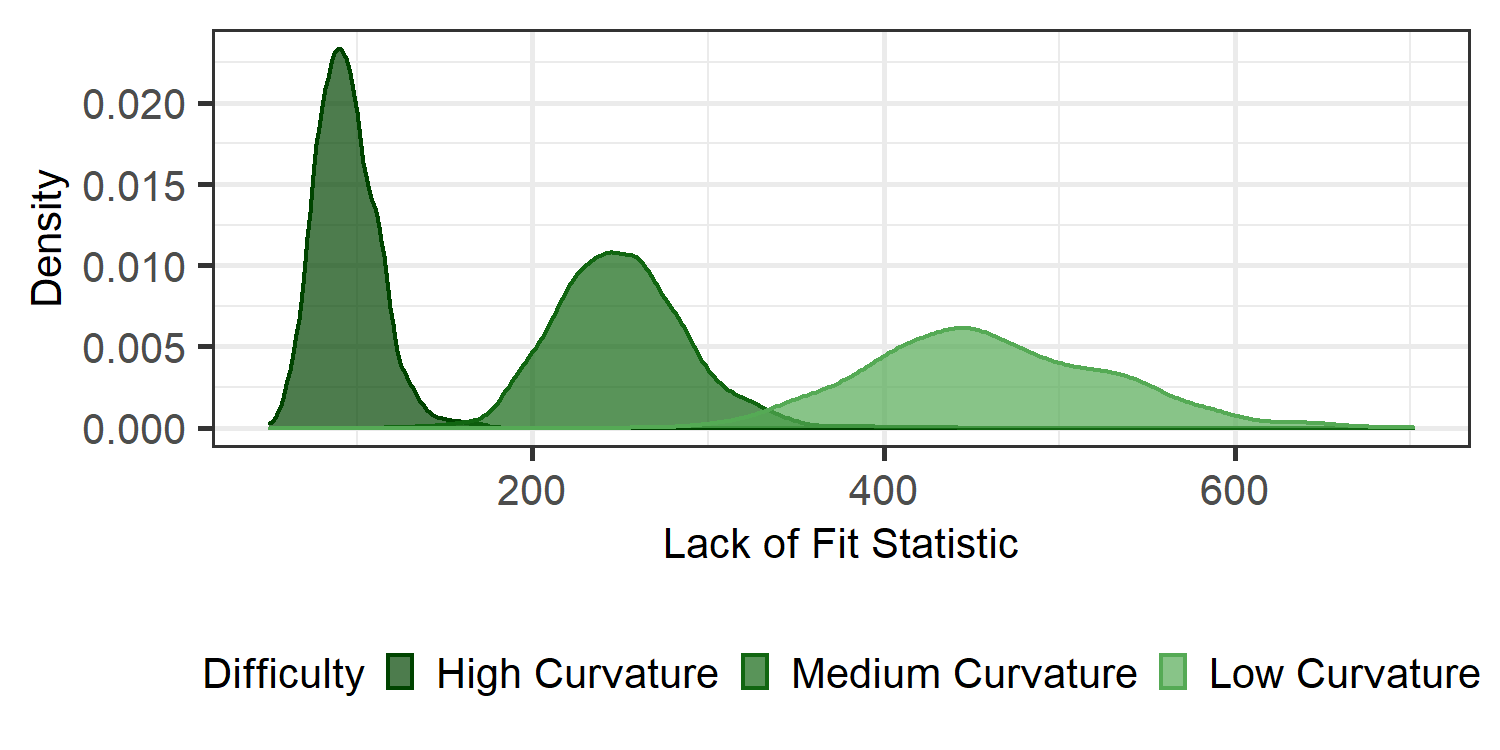
\includegraphics[width=0.75\linewidth,]{thesis_files/figure-latex/lof-density-curves-1} 

}

\caption{Lack of fit statistic density curves}\label{fig:lof-density-curves}
\end{figure}

\begin{table}

\caption{\label{tab:parameter-data}Lineup data simulation final parameters}
\centering
\begin{tabular}[t]{ccccccc}
\toprule
 & $x_{mid}$ & $\hat\alpha$ & $\tilde\alpha$ & $\hat\beta$ & $\hat\theta$ & $\hat\sigma$\\
\midrule
High Curvature & 14.5 & 0.91 & 0.88 & 0.23 & 9.10 & 0.25\\
Medium Curvature & 13.0 & 6.86 & 6.82 & 0.13 & 3.14 & 0.12\\
Low Curvature & 11.5 & 37.26 & 37.22 & 0.06 & -27.26 & 0.05\\
\bottomrule
\end{tabular}
\end{table}

\hypertarget{lineup-setup}{%
\section{Lineup Setup}\label{lineup-setup}}

Lineup plots were generated by mapping one simulated data set corresponding to difficulty level A to a scatter plot to be identified as the target panel while multiple simulated data sets corresponding to difficulty level B were individually mapped to scatter plots for the null panels.
For example, a target plot with simulated data following an increasing exponential curve with high curvature is embedded within null plots with simulated data following an increasing exponential trend with low curvature.
By our constraints, the target panel and null panels will span a similar domain and range.
There are a total of 6 (i.e.~\(3!\cdot 2!\)) lineup curvature combinations.
\cref{fig:curvature-combination-example} illustrates the 6 lineup curvature combinations where the green line indicates the curvature designated to the target panel while the black line indicates the curvature assigned to the null panels.
Two sets of each lineup curvature combination were simulated (total of 12 test data sets) and plotted on both the linear scale and the log scale (total of 24 test lineup plots).
In addition, there are three curvature combinations which generate homogeneous ``Rorschach'' lineups, where all panels are from the same distribution.
Each participant evaluated one of these lineups, but for simplicity, these evaluations are not described in this chapter.

\begin{figure}[tbp]

{\centering 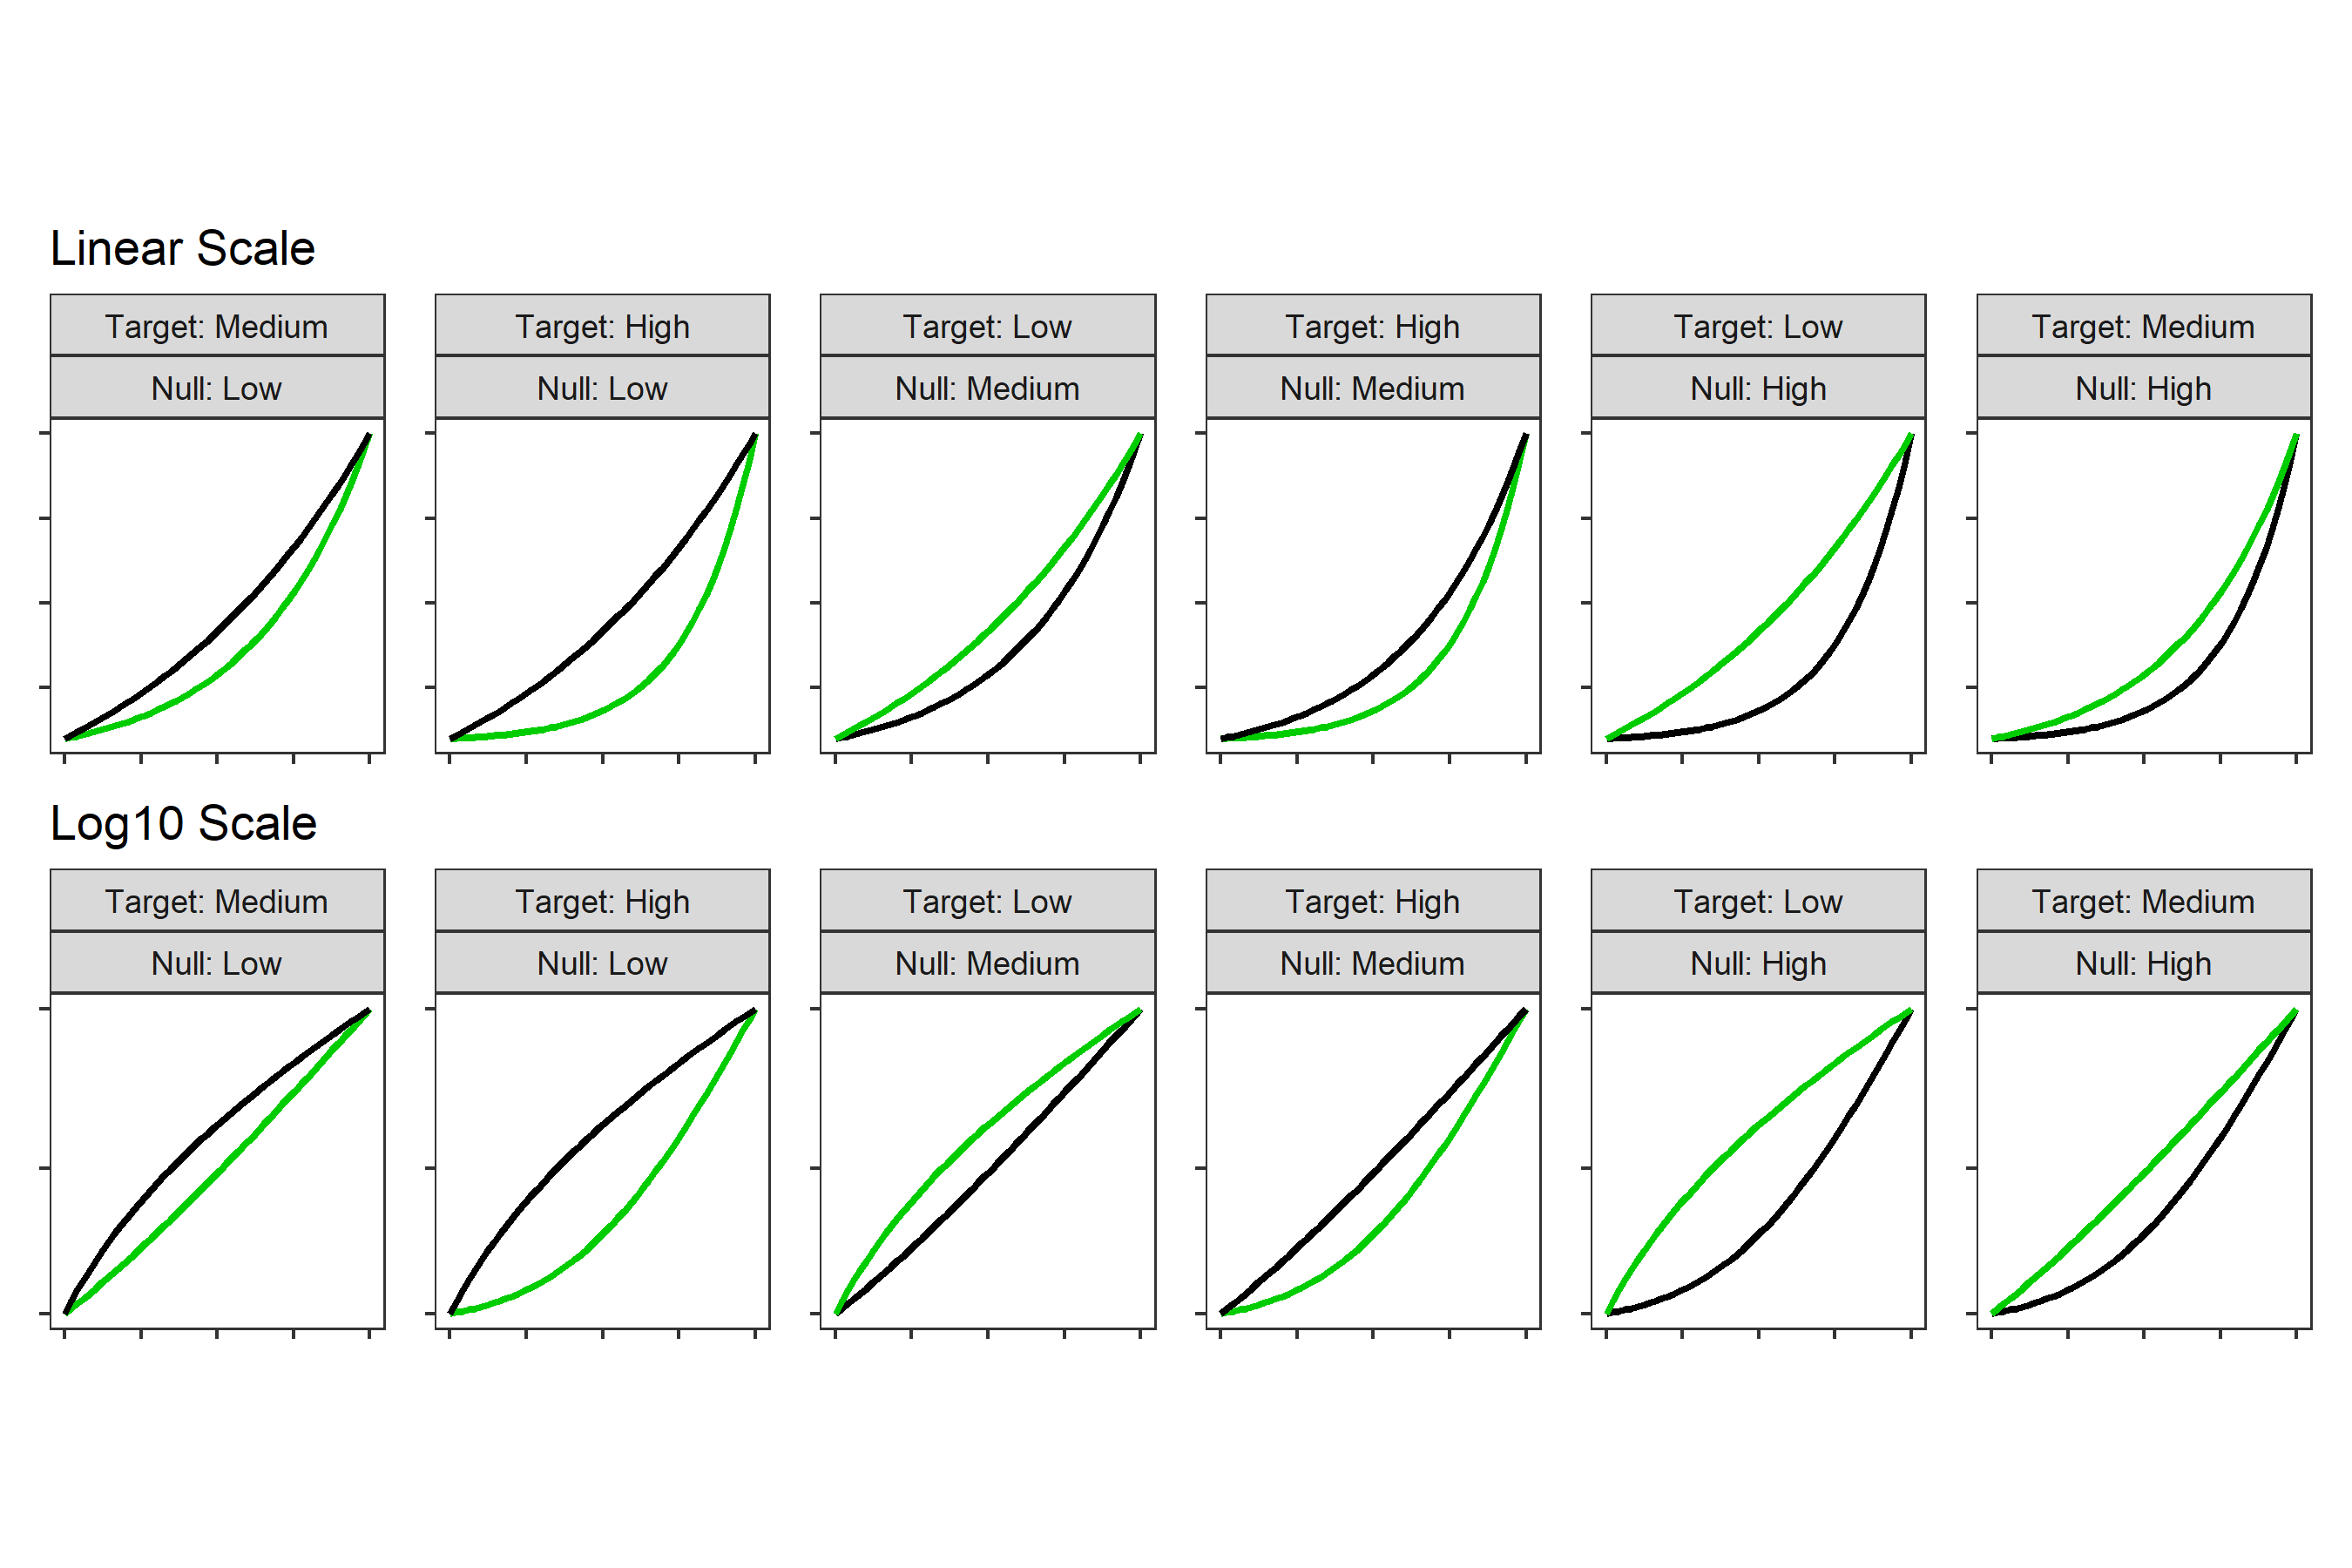
\includegraphics[width=1\linewidth,]{thesis_files/figure-latex/curvature-combination-example-1} 

}

\caption{Lineup curvature combinations}\label{fig:curvature-combination-example}
\end{figure}

\hypertarget{study-design}{%
\section{Study Design}\label{study-design}}

Each participant was shown a total of thirteen lineup plots (12 test lineup plots and 1 Rorschach lineup plot). Participants were randomly assigned one of the two replicate data sets for each of the 6 unique lineup curvature combinations.
For each assigned test data set, the participant was shown the lineup plot corresponding to both the linear scale and the log scale. For the additional Rorschach lineup plot, participants were randomly assigned one data set shown on either the linear or the log scale.
The order of the thirteen lineup plots shown was randomized for each participant.

Participants above the age of majority were recruited from Reddit's Visualization and Sample Size communities.
Since participants recruited on Reddit were not compensated for their time, most participants have an interest in data visualization research.
Previous literature suggests that prior mathematical knowledge or experience with exponential data is not associated with the outcome of graphical experiments (VanderPlas \& Hofmann, 2015).
Participants completed the experiment using a Shiny application found \href{https://shiny.srvanderplas.com/log-study/}{here}.

Participants were shown a series of lineup plots and asked to identify the plot that was most different from the others.
On each plot, participants were asked to justify their choice and provide their level of confidence in their choice.
The goal of this experimental task is to test an individuals ability to perceptually differentiate exponentially increasing trends with differing levels of curvature on both the linear and log scale.

\hypertarget{results}{%
\section{Results}\label{results}}

Participant recruitment through Reddit occurred over the course of two weeks during which 58 individuals completed 518 unique test lineup evaluations.
Previous studies have found that results do not differ on lineup-related tasks between Reddit and e.g.~Amazon Mechanical Turk (VanderPlas \& Hofmann, 2017).
Participants who completed fewer than 6 lineup evaluations were removed from the study (17 participants, 41 evaluations).
The final data set included a total of 41 participants and 477 lineup evaluations.
Each plot was evaluated by between 18 and 28 individuals (Mean: 21.77, SD: 2.29).
In 67\% of the 477 lineup evaluations, participants correctly identified the target panel.

Target plot identification was analyzed using the \texttt{glmer} function in the \texttt{lme4} R package (Bates, Mächler, Bolker, \& Walker, 2015).
Estimates and odds ratio comparisons between the log and linear scales were calculated using the \texttt{emmeans} R package (Lenth, 2021).
Each lineup plot evaluated was assigned a value based on the participant response (correct = 1, not correct = 0).
Define \(Y_{ijkl}\) to be the event that participant \(l = 1,...,N_{participant}\) correctly identifies the target plot for data set \(k = 1,2\) with curvature combination \(j = 1,2,3,4,5,6\) plotted on scale \(i = 1,2\).
The binary response was analyzed using generalized linear mixed model following a binomial distribution with a logit link function following a row-column blocking design accounting for the variation due to participant and data set respectively as
\begin{equation}
\text{logit }P(Y_{ijk}) = \eta + \delta_i + \gamma_j + \delta \gamma_{ij} + s_l + d_k
\end{equation}
\noindent where

\begin{itemize}
\item $\eta$ is the baseline average probability of selecting the target plot
\item $\delta_i$ is the effect of the log/linear scale
\item $\gamma_j$ is the effect of the curvature combination
\item $\delta\gamma_{ij}$ is the two-way interaction effect of the scale and curvature
\item $s_l \sim N(0,\sigma^2_\text{participant})$, random effect for participant characteristics
\item $d_k \sim N(0,\sigma^2_{\text{data}})$, random effect for data specific characteristics. 
\end{itemize}

\noindent We assume that random effects for data set and participant are independent.

The analysis of variance table shown in \cref{tab:lineup-anova-table} indicates a significant interaction between the curvature combination and scale. Variance due to participant and data set were estimated to be \(\sigma^2_{\text{participant}} = 2.79\) (s.e. 1.67) and \(\sigma^2_{\text{data}} = 0.44\) (s.e. 0.66) respectively.

\begin{table}

\caption{\label{tab:lineup-anova-table}Lineup ANOVA table for fixed effects.}
\centering
\begin{tabular}[t]{cccc}
\toprule
Effect & Chisq & Df & Pr..Chisq.\\
\midrule
Curvature & 19.96 & 5 & 0.00127\\
Scale & 14.43 & 1 & 0.00015\\
Curvature x Scale & 33.65 & 5 & <0.0001\\
\bottomrule
\end{tabular}
\end{table}

On both the log and linear scales, the highest accuracy occurred in lineup plots where the target model and null model had large curvature differences (i.e.~high curvature target panel embedded in low curvature null panels; low curvature target panel embedded in high curvature null panels).
There is a decrease in accuracy on the linear scale when comparing a target plot with less curvature to null plots with more curvature (i.e.~medium curvature target panel embedded in high curvature null panels; low curvature target panel embedded in medium curvature null panels).
Best, Smith, \& Stubbs (2007) found that accuracy of identifying the correct curve type was higher when nonlinear trends were presented indicating that it is hard to say something is linear (i.e.~something has less curvature), but easy to say that it is not linear; our results concur with this observation.
Overall, there are no significant differences in accuracy between curvature combinations when data is presented on a log scale indicating participants were consistent in their success of identifying the target panel on the log scale.
\cref{fig:odds-ratio-plot} displays the estimated (log) odds ratio of successfully identifying the target panel on the log scale compared to the linear scale.
The choice of scale has no impact if curvature differences are large (i.e.~low curvature and high curvature combinations).
However, presenting data on the log scale makes us more sensitive to slight changes in curvature (i.e.~high curvature target panel embedded in medium curvature null panels; medium curvature target panel embedded in high curvature null panels; low curvature target panel embedded in medium curvature null panels).
An exception occurs when identifying a plot with curvature embedded in null plots close to a linear trend (i.e.~medum curvature target panel embedded in low curvature null panels), again supporting the claim that it is easy to identify a curve in a bunch of lines but much harder to identify a line in a bunch of curves (Best, Smith, \& Stubbs, 2007).

\begin{figure}[tbp]

{\centering 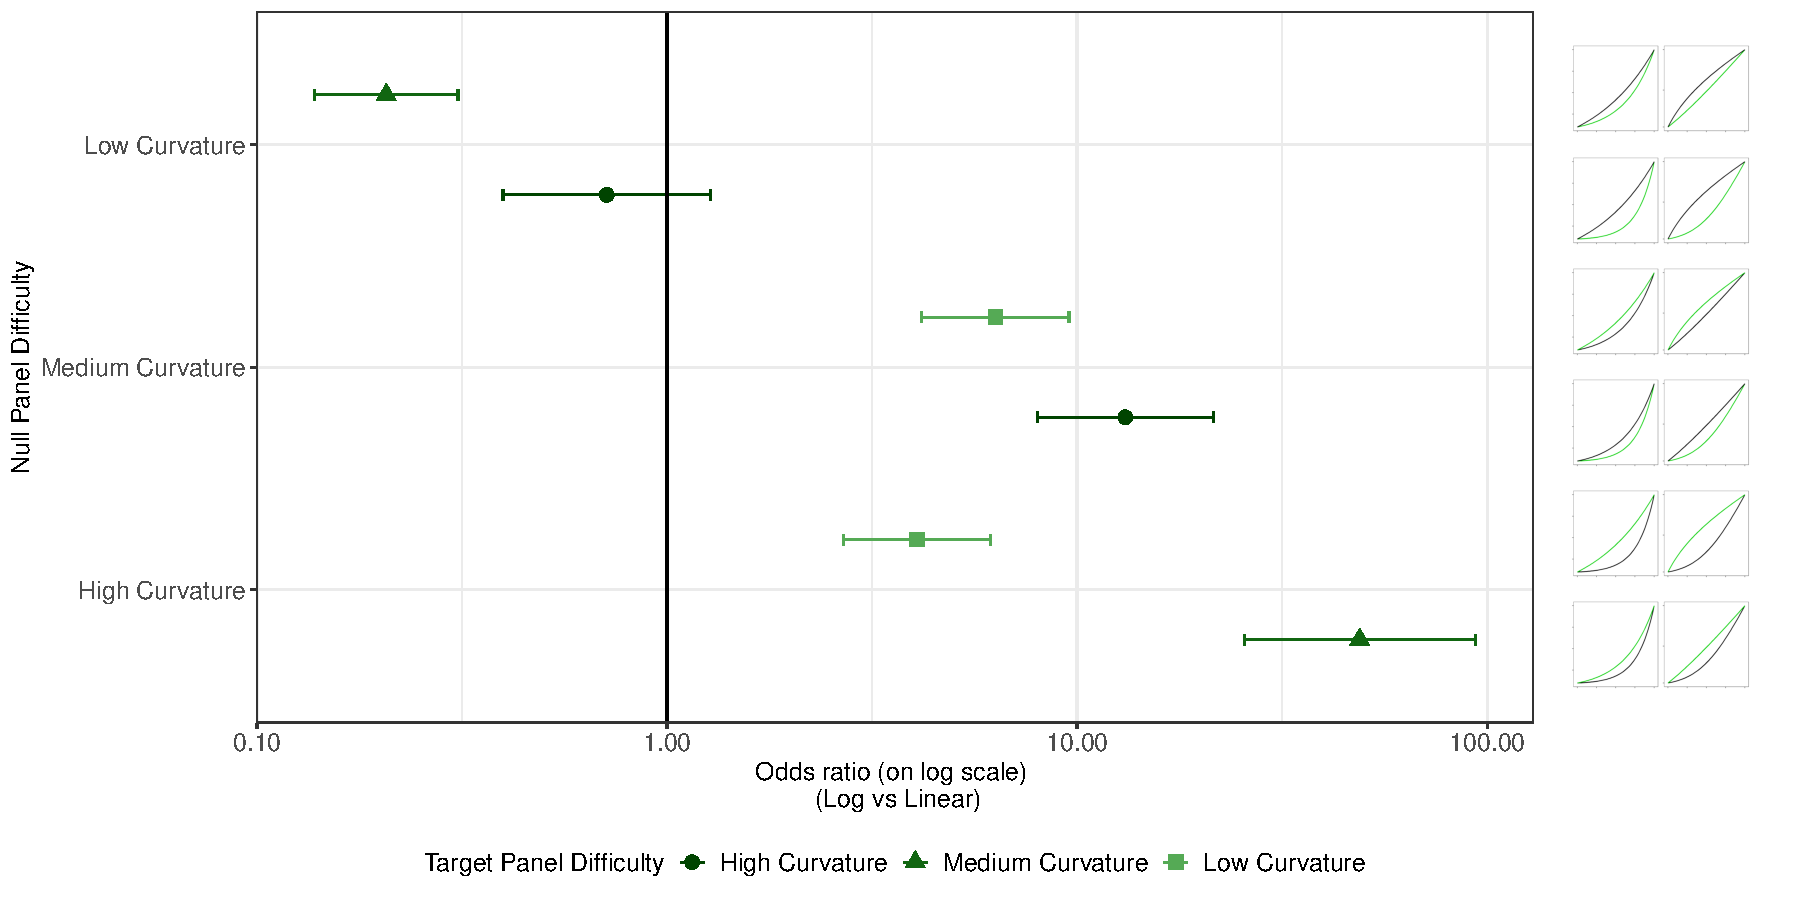
\includegraphics[width=\linewidth,]{thesis_files/figure-latex/odds-ratio-plot-1} 

}

\caption{Lineups log(odds) results}\label{fig:odds-ratio-plot}
\end{figure}

\hypertarget{discussion-and-conclusion}{%
\section{Discussion and Conclusion}\label{discussion-and-conclusion}}

The overall goal of this chapter is to provide basic research to support the principles used to guide design decisions in scientific visualizations of exponential data.
In this study, we explore the use of linear and log scales to determine whether our ability to notice differences in exponentially increasing trends is impacted by the choice of scale.
Our results indicated that when there was a large difference in curvature between the target plot and null plots, the choice of scale had no impact and participants accurately differentiated between the two curves on both the linear and log scale.
However, displaying exponentially increasing data on a log scale improved the accuracy of differentiating between models with slight curvature differences.
An exception occurred when identifying a plot with curvature embedded in surrounding plots closely relating to a linear trend, indicating that it is easy to identify a curve in a group of lines but much harder to identify a line in a group of curves.
The use of visual inference to identify these guidelines suggests that there are \emph{perceptual} advantages to log scales when differences are subtle.
What remains to be seen is whether there are cognitive disadvantages to log scales: do log scales make it harder to make use of graphical information?

\hypertarget{youdrawit}{%
\chapter{Prediction with you draw it}\label{youdrawit}}

\hypertarget{introduction-1}{%
\section{Introduction}\label{introduction-1}}

In \protect\hyperlink{lineups}{Chapter 2}, a base foundation for future exploration of the use of log scales was established by evaluating participants ability to identify differences in charts through the use of lineups.
This did not require that participants were able to understand exponential growth, identify log scales, or have any mathematical training; instead, it simply tested the change in perceptual sensitivity resulting from visualization choices.
In order to determine whether there are cognitive disadvantages to log scales, we utilize interactive graphics to test an individual's ability to make predictions for exponentially increasing data. In this study, participants are asked to draw a line using their computer mouse through the exponentially increasing trend shown on both the log and linear scale.

\hypertarget{past-methodology}{%
\subsection{Past Methodology}\label{past-methodology}}

Initial studies in the 20th century explored the use of fitting lines by eye through a set of points (Finney, 1951; Mosteller, Siegel, Trapido, \& Youtz, 1981).
Common methods of fitting trends by eye involve maneuvering a string, black thread, or ruler until the fit is suitable, then drawing the line.
In Finney (1951), it was of interest to determine the effect of stopping iterative maximum likelihood calculations after one iteration. Twenty-one scientists were recruited via postal mail and asked to ``rule two lines'' in order to judge by eye the positions for a pair of parallel probit regression lines in a biological assay \pcref{fig:subjective-judgement}.
Results indicated that one cycle of iterations was sufficient based on the starting values provided by eye from the participants.

\begin{figure}[tbp]

{\centering 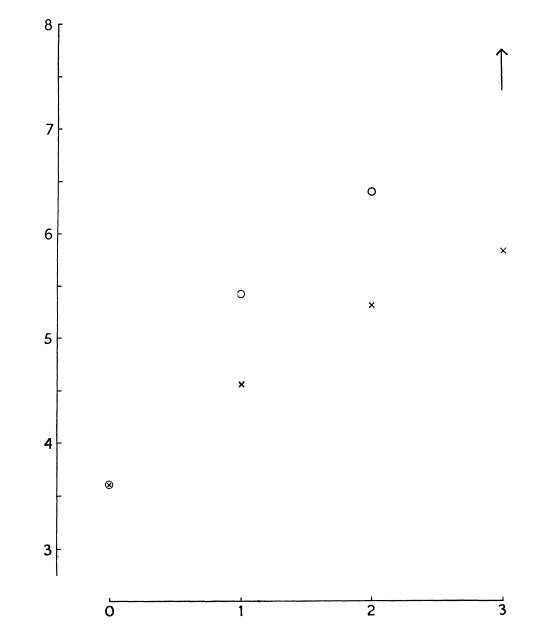
\includegraphics[width=0.5\linewidth,]{images/subjective-judgement-plot} 

}

\caption{Subjective Judgement in Statistical Analysis (1951) Parallel Probits}\label{fig:subjective-judgement}
\end{figure}

Thirty years later, Mosteller, Siegel, Trapido, \& Youtz (1981), sought to understand the properties of least squares and other computed lines by establishing one systematic method of fitting lines by eye.
The authors recruited 153 graduate students and post doctoral researchers in Introductory Biostatistics.
Participants were asked to fit lines by eye to four sets of points \pcref{fig:mosteller-eyefitting-plot} using an 8.5 x 11 inch transparency with a straight line etched completely across the middle.
A latin square design with packets of the set of points stapled together in four different sequences was used to determine if there is an effect of order of presentation.
It was found that order of presentation had no effect and that participants tended to fit the slope of the first principal component over the slope of the least squares regression line.

\begin{figure}[tbp]

{\centering 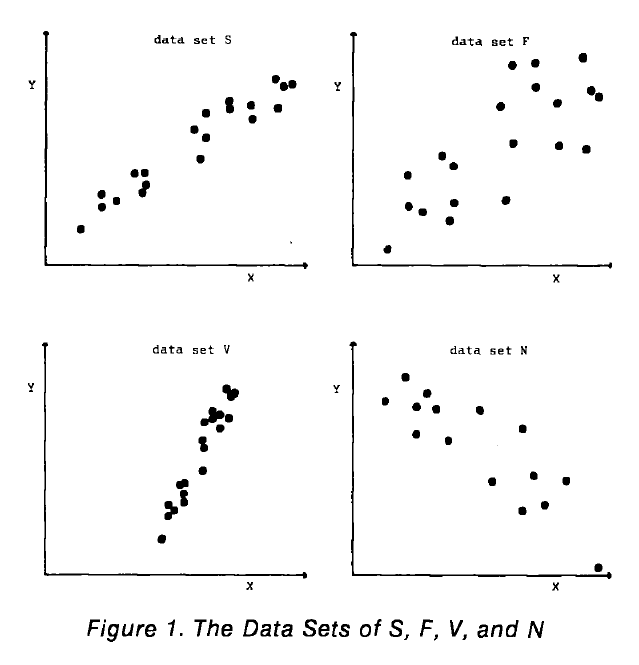
\includegraphics[width=0.7\linewidth,]{images/eyefitting-straight-lines-plots} 

}

\caption{Eye Fitting Straight Lines (1981) Data Sets}\label{fig:mosteller-eyefitting-plot}
\end{figure}

In 2015, the New York Times introduced an interactive feature, called You Draw It (Aisch, Cox, \& Quealy, 2015; Buchanan, Park, \& Pearce, 2017; Katz, 2017)
Readers are asked to input their own assumptions about various metrics and compare how these assumptions relate to reality.
The NY Times team utilizes Data Driven Documents (D3) that allows readers to predict these metrics through the use of drawing a line on their computer screen with their computer mouse.
\cref{fig:nyt-caraccidents} is one such example in which readers are asked to draw the line for the missing years providing what they estimate to be the number of Americans who have died every year from car accidents, since 1990.
After the reader has completed drawing the line, the actual observed values are revealed and the reader may check their estimated knowledge against the actual reported data (Katz, 2017).

\begin{figure}[tbp]

{\centering 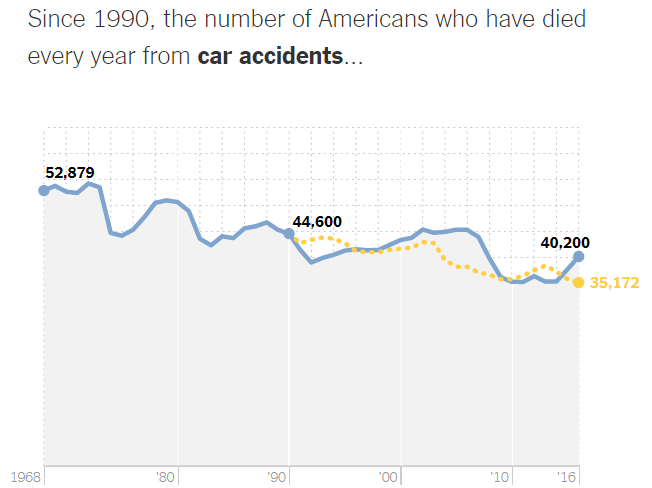
\includegraphics[width=0.75\linewidth,]{images/nyt-caraccidents-frame4} 

}

\caption{New York Times You Draw It Feature}\label{fig:nyt-caraccidents}
\end{figure}

\hypertarget{data-driven-documents}{%
\subsection{Data Driven Documents}\label{data-driven-documents}}

Major news and research organizations such as the NY Times, FiveThirtyEight, Washing Post, and the Pew Research Center create and customize graphics with Data Driven Documents (D3).
In June 2020, the NY Times released a front page displaying figures that represent each of the 100,000 lives lost from the coronavirus pandemic until this point in time (Barry et al., 2020); this visualization was meant to bring about a visceral reaction and resonate with readers.
During 2021 March Maddness, FiveThirtyEight created a roster-shuffling machine which allowed readers to build their own NBA contender through interactivity (Ryanabest, 2021).
Data Driven Documents (D3) is an open-source JavaScript based graphing framework created by Mike Bostock during his time working on graphics at the NY Times.
For readers familiar with R, it is notable to consider D3 in JavaScript equivalent to the ggplot2 package in R.
Similar to geometric objects and style choices in ggplot2, the grammar of D3 also includes elements such as circles, paths, and rectangles with choices of attributes and styles such as color and size.
Data Driven Documents depend on Extensible Markup Langage (XML) to generate graphics and images by binding objects and layers to the plotting area as Scalable Vector Graphics (SVG) in order to preserve the shapes rather than the pixels \pcref{fig:raster-vs-vector} (Tol, 2021)
Advantages of using D3 include animation and allowing for movement and user interaction such as hovering, clicking, and brushing.

\begin{figure}[tbp]

{\centering 
\includegraphics[width=0.7\linewidth,]{images/raster-vs-vector} 

}

\caption{SVG vs Raster}\label{fig:raster-vs-vector}
\end{figure}

A challenge of working with D3 is the environment necessary to display the graphics and images.
The r2d3 package in R provides an efficient integration of D3 visuals and R by displaying them in familiar HTML output formats such as RMarkdown or Shiny applications (Luraschi \& Allaire, 2018).
The creator of the graphic applies D3.js source code to visualize data which has previously been processed within an R setting.

The example R code illustrates the structure of the r2d3 function which includes specification of a data frame in R (converted to a JSON file), the D3.js source code file, and the D3 version that accompanies the source code.
A default SVG container for layering elements is then generated by the r2d3 function which renders the plot using the source code.
\protect\hyperlink{youdrawit-with-shiny}{Appendix A} outlines the development of the you draw interactive plots used in this study through the use of r2d3 and R shiny applications.
\cref{fig:youdrawit-example} provides an example of a you draw it interactive plot as seen by participants during the study.
The first frame shows what the participant sees along with the prompt, ``Use your mouse to fill in the trend in the yellow box region.''
Next, the yellow box region moves along as the participant draws their trend-line until the yellow region disappears indicating the participant has filled in the entire domain.

\begin{Shaded}
\begin{Highlighting}[]
\FunctionTok{r2d3}\NormalTok{(}\AttributeTok{data =}\NormalTok{ data, }\AttributeTok{script =} \StringTok{"d3{-}source{-}code.js"}\NormalTok{, }
    \AttributeTok{d3\_version =} \StringTok{"5"}\NormalTok{)}
\end{Highlighting}
\end{Shaded}

\begin{figure}[tbp]

{\centering 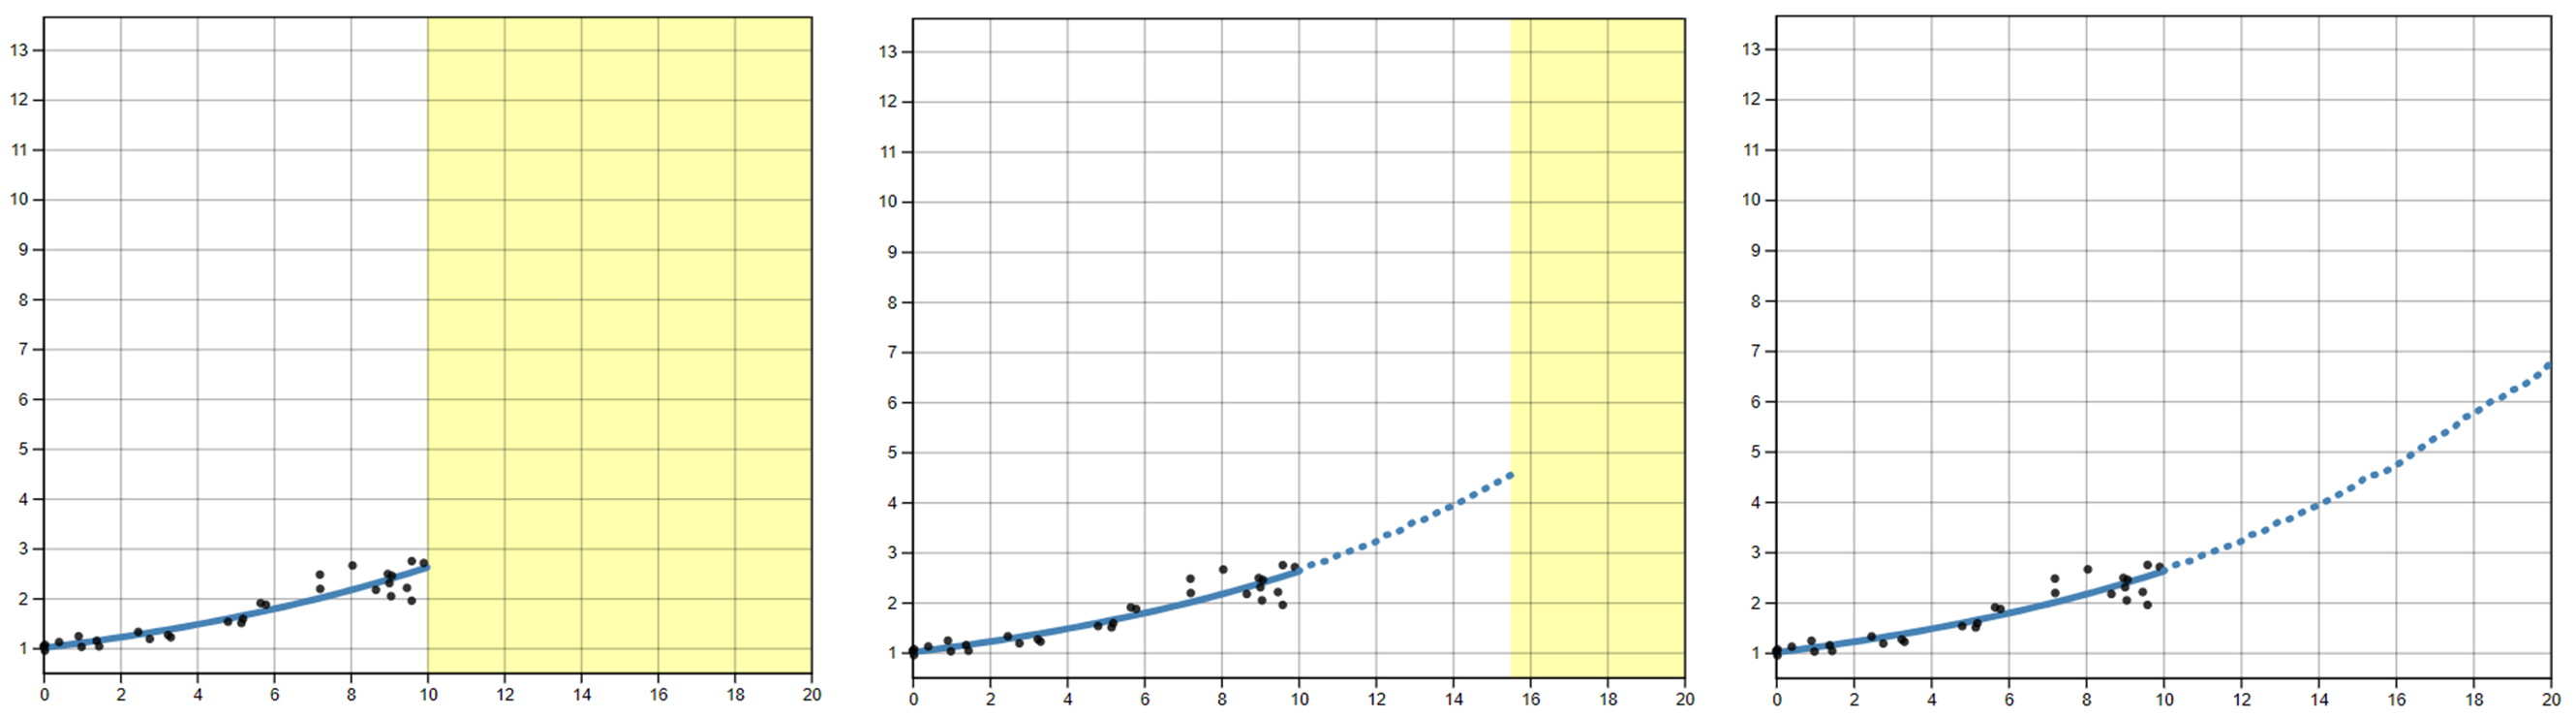
\includegraphics[width=1\linewidth,]{images/ydiExample-0.10-10-linear} 

}

\caption{You Draw It Example}\label{fig:youdrawit-example}
\end{figure}

\hypertarget{study-design-1}{%
\section{Study Design}\label{study-design-1}}

This chapter contains two sub-studies; the first aims to establish you draw it as a tool for measuring predictions of trends fitted by eye and the second then applies you draw it as a method for testing graphics.
Mosteller, Siegel, Trapido, \& Youtz (1981) was replicated as part of the study data collection in order to validate you draw it as a method for testing graphics, referred to as Eye Fitting Straight Lines in the Modern Era.
This method is then used to test an individual's ability to make predictions for exponentially increasing data on both the log and linear scales, referred to as Prediction of Exponential Trends.
Data for both sub-studies were collected in conjunction with one another over the same study participant sample.

A total of 6 data sets - 4 Eye Fitting Straight Lines in the Modern Era and 2 Prediction of Exponential Trends - are generated for each individual at the start of the experiment.
The 2 simulated data sets corresponding to the simulated data models used in the Prediction of Exponential Trends sub-study are then plotted a total of 4 times each with different aesthetic and scale choices for a total of 8 task plots.
Participants in the study are first shown 2 you draw it practice plots followed by 12 you draw it task plots.
The order of all 12 task plots was randomly assigned for each individual in a completely randomized design where users saw the 4 task plots from the Eye Fitting Straight Lines in the Modern Era sub-study interspersed with the 8 task plots from the Prediction of Exponential Trends sub-study.

Participants completed the experiment using a RShiny application found \href{https://shiny.srvanderplas.com/you-draw-it/}{here}.
Participants were recruited through Twitter, Reddit, and direct email during May 2021.
A total of 39 individuals completed 256 unique you draw it task plots.
All completed you draw it task plots were included in the analysis.

\hypertarget{eye-fitting-straight-lines-in-the-modern-era}{%
\section{Eye Fitting Straight Lines in the Modern Era}\label{eye-fitting-straight-lines-in-the-modern-era}}

Finney (1951) and Mosteller, Siegel, Trapido, \& Youtz (1981) use methods such as using a ruler, string, or transparency sheet to fit straight lines through a set of points.
This section replicates the study found in Mosteller, Siegel, Trapido, \& Youtz (1981) in order to establish you draw it as a tool and method for testing graphics.

\hypertarget{data-generation-1}{%
\subsection{Data Generation}\label{data-generation-1}}

All data processing was conducted in R before being passed to the D3.js source code.
A total of \(N = 30\) points \((x_i, y_i), i = 1,...N\) were generated for \(x\in [x_{min}, x_{max}]\) where \(x\) and \(y\) have a linear relationship.
Data was simulated based on linear model with additive errors:
\begin{align}
y_i & = \beta_0 + \beta_1 \cdot x_i + e_i \\
\text{with } e_i & \sim N(0, \sigma^2). \nonumber
\end{align}
The parameters \(\beta_0\) and \(\beta_1\) are selected to replicate Mosteller, Siegel, Trapido, \& Youtz (1981) with \(e_i\) generated by rejection sampling in order to guarantee the points shown align with that of the fitted line.
An ordinary least squares regression is then fit to the simulated points in order to obtain the best fit line and fitted values in 0.25 increments across the domain, \((x_k, \hat y_{k,OLS}), k = 1, ..., 4\cdot x_{max} +1\).
The data simulation function then outputs a list of point data and line data both indicating the parameter identification, x value, and corresponding simulated or fitted y value.
The data simulation procedure is described in \cref{alg:eyefitting-algorithm}.

\begin{algorithm}
  \caption{Eye Fitting Straight Lines in the Modern Era Data Simulation}\label{alg:eyefitting-algorithm}
  \begin{algorithmic}[1]
    \Statex \textbullet~\textbf{Input Parameters:} $y_{\bar{x}}$ for calculating the y-intercept, $\beta_0$; slope $\beta_1$; standard deviation from line $\sigma$; sample size $N = 30$; domain $x_{min}$ and $x_{max}$; fitted value increment $x_{by} = 0.25$.
    \Statex \textbullet~\textbf{Output Parameters:} List of point data and line data each indicating the parameter identification, x value, and corresponding simulated or fitted y value.
    \State Randomly select and jitter N = 30 x-values along the domain, $x_{i=1:N}\in [x_{min}, x_{max}]$.
    \State Determine the y-intercept, $\beta_0$, at x = 0 from the provided slope ($\beta_1$) and y-value at the mean of x ($y_{\bar{x}}$) using point-slope equation of a line.
    \State Generate "good" errors, $e_{i = 1:n}$ based on $N(0,\sigma)$ by setting a constraint requiring the mean of the first N/3 errors $< |2\sigma|.$
    \State Simulate point data based on $y_i = \beta_0 + \beta_1 x_i + e_i$
    \State Obtain ordinary least squares regression coefficients, $\hat\beta_0$ and $\hat\beta_1$, for the simulated point data using the `lm` function in the base stats R package.
    \State Obtain fitted values every 0.25 increment across the domain from the ordinary least squares regression $\hat y_{k,OLS} = \hat\beta_{0,OLS} + \hat\beta_{1,OLS} x_k$.
    \State Output data list of point data and line data each indicating the parameter identification, x value, and corresponding simulated or fitted y value.
  \end{algorithmic}
\end{algorithm}

Simulated model equation parameters were selected to reflect the four data sets (F, N, S, and V) used in Mosteller, Siegel, Trapido, \& Youtz (1981) \pcref{tab:eyefitting-parameters}.
Parameter choices F, N, and S simulated data across a domain of 0 to 20.
Parameter choice F produces a trend with a positive slope and a large variance while N has a negative slope and a large variance.
In comparison, S shows a trend with a postive slope with a small variance and V yields a steep positive slope with a small variance over the domain of 4 to 16.
\cref{fig:eyefitting-simplot} illustrates an example of simulated data for all four parameter choices intended to reflect the trends seen in \cref{fig:mosteller-eyefitting-plot}.
Within the interactive plot code, the aspect ratio defining the x to y axis ratio was set to 1 with a consistent y range buffer of 10\% to allow for users to draw outside the data set range.

\begin{table}

\caption{\label{tab:eyefitting-parameters}Eye Fitting Straight Lines in the Modern Era simulation model parameters}
\centering
\begin{tabular}[t]{cccc}
\toprule
Parameter Choice & $y_{\bar{x}}$ & $\beta_1$ & $\sigma$\\
\midrule
S & 3.88 & 0.66 & 1.30\\
F & 3.90 & 0.66 & 1.98\\
V & 3.89 & 1.98 & 1.50\\
N & 4.11 & -0.70 & 2.50\\
\bottomrule
\end{tabular}
\end{table}

\begin{figure}[tbp]

{\centering 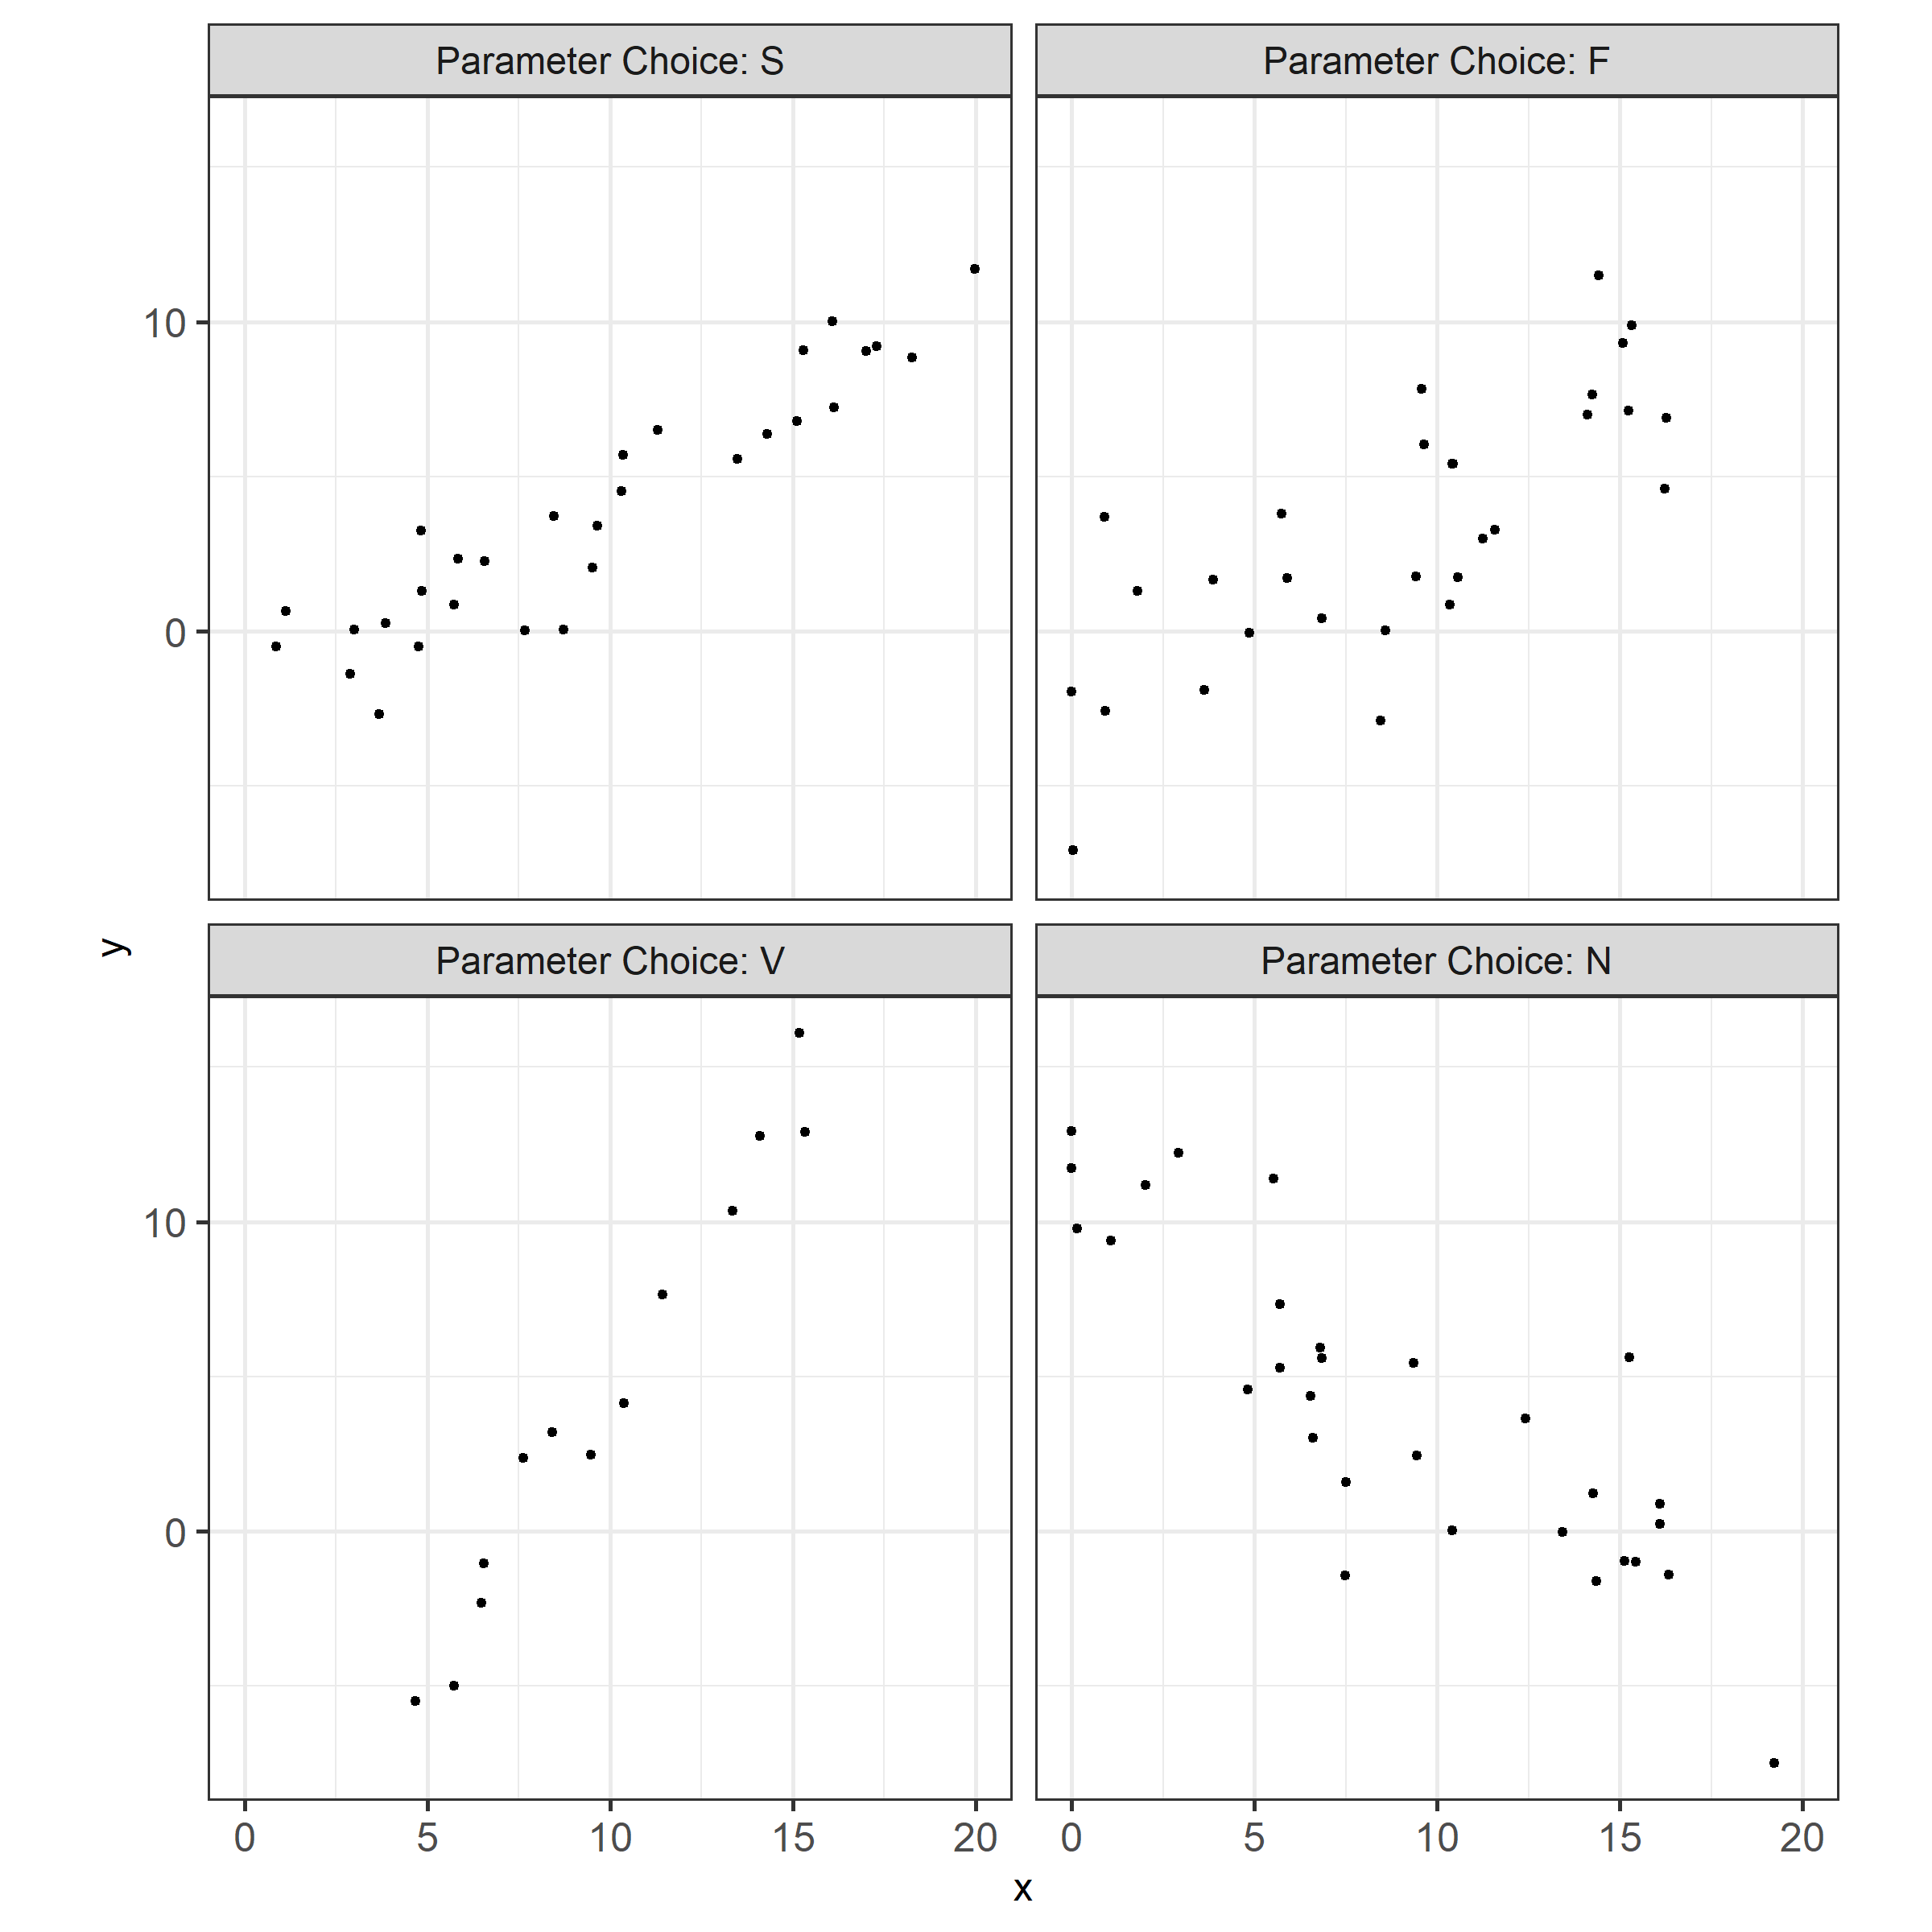
\includegraphics[width=0.75\linewidth,]{thesis_files/figure-latex/eyefitting-simplot-1} 

}

\caption{Eye Fitting Straight Lines in the Modern Era Simulated Data Example}\label{fig:eyefitting-simplot}
\end{figure}

\hypertarget{results-1}{%
\subsection{Results}\label{results-1}}

In addition to the participant drawn points, \((x_k, y_{drawn})\), and the ordinary least squares (OLS) regression fitted values, \((x_k, \hat y_{k,OLS})\), a regression equation with a slope based on the first principal component (PCA) was used to calculate fitted values, \((x_k, \hat y_{k,PCA})\).
For each set of simulated data and parameter combination, the PCA regression equation was determined by using the princomp function in the base R stats package to obtain the rotations of the first principal component for vectors x and y.
The estimated slope, \(\hat\beta_{1,PCA}\), is determined by the ratio of the y rotation and x rotation of the first principal component with the y-intercept, \(\hat\beta_{0,PCA}\) calculated by the point-slope equation of a line using the mean of of the simulated points, \((\bar x_i, \bar y_i)\).
Fitted values, \(\hat y_{k,PCA}\) are then obtained every 0.25 increment across the domain from the PCA regression equation, \(\hat y_{k,PCA} = \hat\beta_{0,PCA} + \hat\beta_{1,PCA} x_k\).
\cref{fig:ols-vs-pca-example} illustrates the difference between an OLS regression equation which minimizes the vertical distance of points from the line and a regression equation with a slope calculated by the first principal component which minimizes the smallest distance of points from the line.

\begin{figure}[tbp]

{\centering 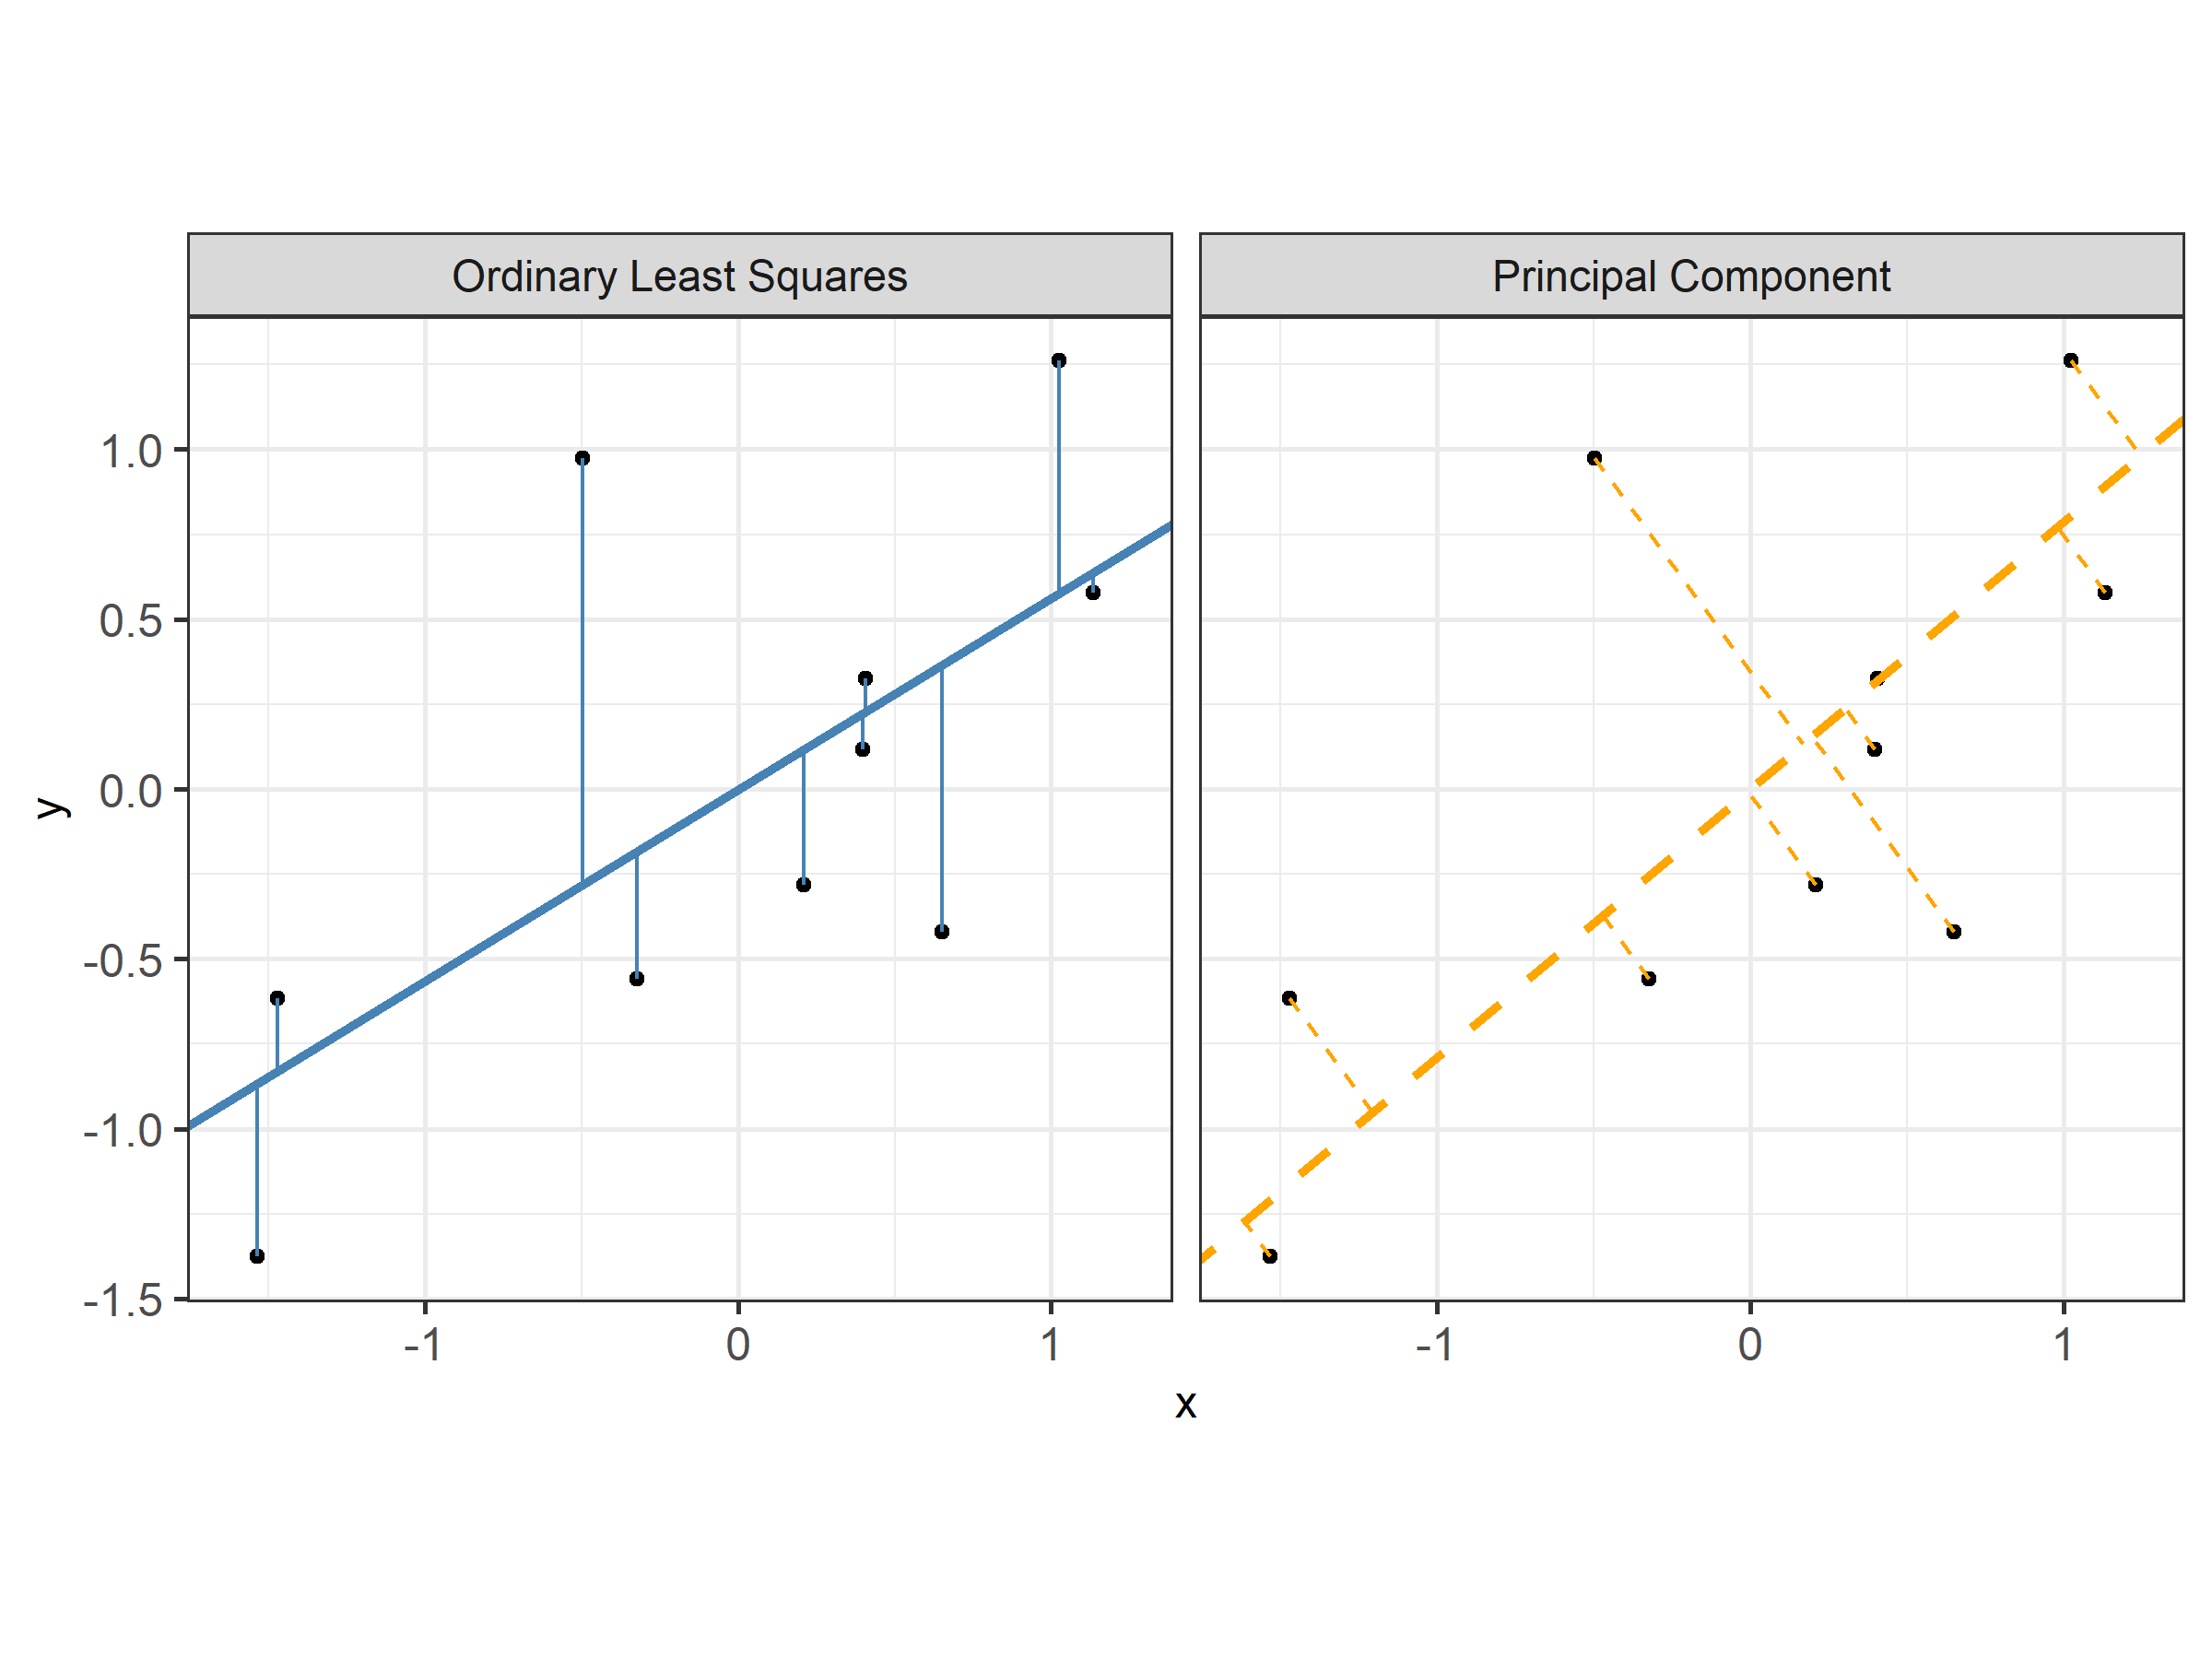
\includegraphics[width=0.9\linewidth,]{thesis_files/figure-latex/ols-vs-pca-example-1} 

}

\caption{OLS vs PCA Regression Lines}\label{fig:ols-vs-pca-example}
\end{figure}

For each participant, the final data set used for analysis contains \(x_{ijk}, y_{ijk,drawn}, \hat y_{ijk,OLS}\), and \(\hat y_{ijk,PCA}\) for parameter choice \(i = 1,2,3,4\), j = \(1,...N_{participant}\), and \(x_{k}\) value \(k = 1, ...,4\cdot x_{max} + 1\).
Using both a linear mixed model and a generalized additive mixed model, comparisons of vertical residuals in relation to the OLS fitted values (\(e_{k,OLS} = y_{k,drawn} - \hat y_{k,OLS}\)) and PCA fitted values (\(e_{k,PCA} = y_{k,drawn} - \hat y_{k,PCA}\)) were made across the domain of x.
\cref{fig:eyefitting-example-plot} displays an example of all three fitted trend lines for parameter choice F.

\begin{figure}[tbp]

{\centering 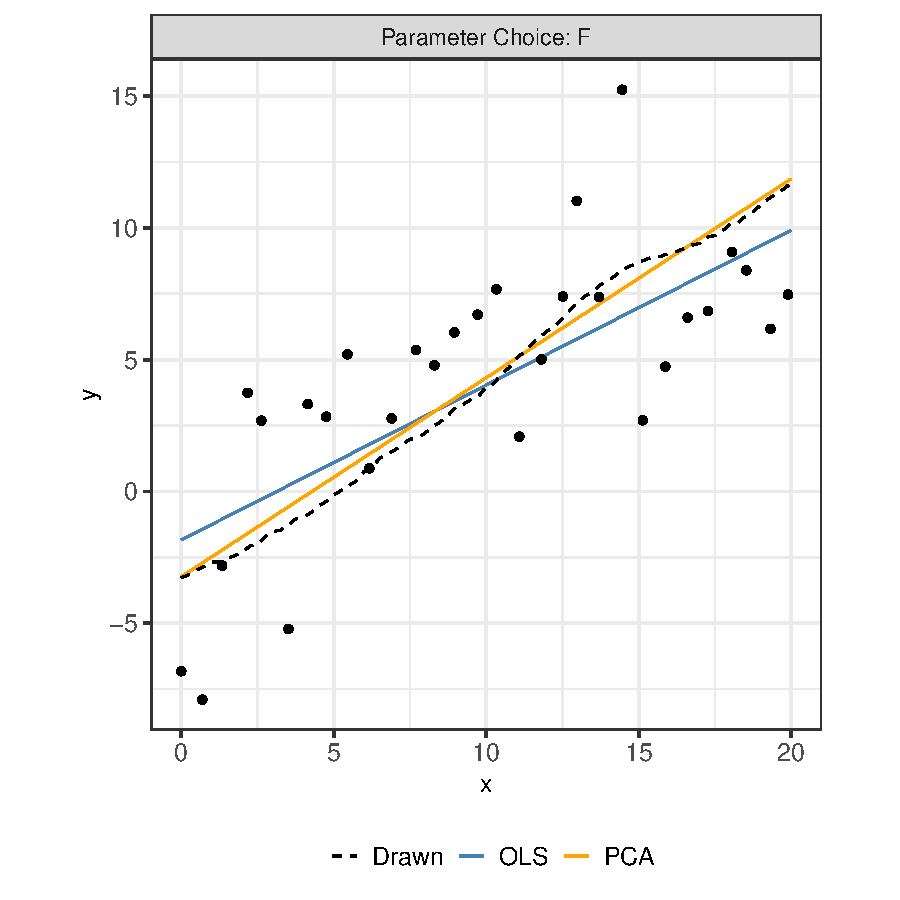
\includegraphics[width=0.65\linewidth,]{thesis_files/figure-latex/eyefitting-example-plot-1} 

}

\caption{Eye Fitting Straight Lines in the Modern Era Example}\label{fig:eyefitting-example-plot}
\end{figure}

Using the lmer function in the lme4 package (Bates, Mächler, Bolker, \& Walker, 2015), a linear mixed model (LMM) is fit separately to the OLS and PCA residuals, constraining the fit to a linear trend.
Parameter choice, \(x\), and the interaction between \(x\) and parameter choice were treated as fixed effects with a random participant effect accounting for variation due to participant.
The LMM equation for each fit (OLS and PCA) residuals is given by:
\begin{equation}
y_{ijk,drawn} - y_{ijk,fit} = e_{ijk,fit} = \left[\gamma_0 + \alpha_i\right] + \left[\gamma_{1} x_{ijk} + \gamma_{2i} x_{ijk}\right] + p_{j} + \epsilon_{ijk}
\end{equation}
\noindent where

\begin{itemize}
\tightlist
\item
  \(\gamma_0\) is the overall intercept
\item
  \(\alpha_i\) is the effect of the parameter choice on the intercept
\item
  \(\gamma_1\) is the overall slope for \(x\)
\item
  \(\gamma_{2i}\) is the effect of the parameter choice on the slope
\item
  \(p_{j} \sim N(0, \sigma^2_{participant})\) is the random error due to participant variation
\item
  \(\epsilon_{ij} \sim N(0, \sigma^2)\) is the residual error.
\end{itemize}

Eliminating the linear trend constraint, the bam function in the mgcv package (S. N. Wood, 2003, 2004, 2011; S. N. Wood, 2017; S. N. Wood, N., Pya, \& Saefken, 2016) is used to fit a generalized additive mixed model (GAMM) separately to the OLS and PCA residuals to allow for estimation of smoothing splines.
Parameter choice was treated as a fixed effect with no estimated intercept and a separate smoothing spline for \(x\) was estimated for each parameter choice. A random participant effect accounting for variation due to participant and a random spline for each participant accounted for variation in spline for each participant.
The GAMM equation for each fit (OLS and PCA) residuals is given by:
\begin{equation}
y_{ijk, drawn} - y_{ijk, fit} = e_{ijk,fit} = \alpha_i + s_{i}(x_{ijk}) + p_{j} + s_{j}(x_{ijk})
\end{equation}
\noindent where

\begin{itemize}
\tightlist
\item
  \(\alpha_i\) is the intercept for the parameter choice \(i\)
\item
  \(s_{i}\) is the smoothing spline for the \(i^{th}\) parameter combination
\item
  \(p_{j} \sim N(0, \sigma^2_{participant})\) is the error due to participant variation
\item
  \(s_{j}\) is the random smoothing spline for each participant.
\end{itemize}

\cref{fig:eyefitting-lmer-residualplots} and \cref{fig:eyefitting-gamm-residualplots} show the estimated trends of residuals (vertical deviation of participant drawn points from both the OLS and PCA fitted points) as modeled by a LMM and GAMM respectively.
Examining the plots, the estimated trends of PCA residuals (orange) appear to align closer to the \(y=0\) horizontal (dashed) line than the OLS residuals (blue).
In particular, this trend is more prominent in parameter choices with large variances (F and N).
These results are consistent to those found in Mosteller, Siegel, Trapido, \& Youtz (1981) indicating participants fit a trend line closer to the estimated regression line with the slope of the first principal component than the estimated OLS regression line.

\begin{figure}[tbp]

{\centering 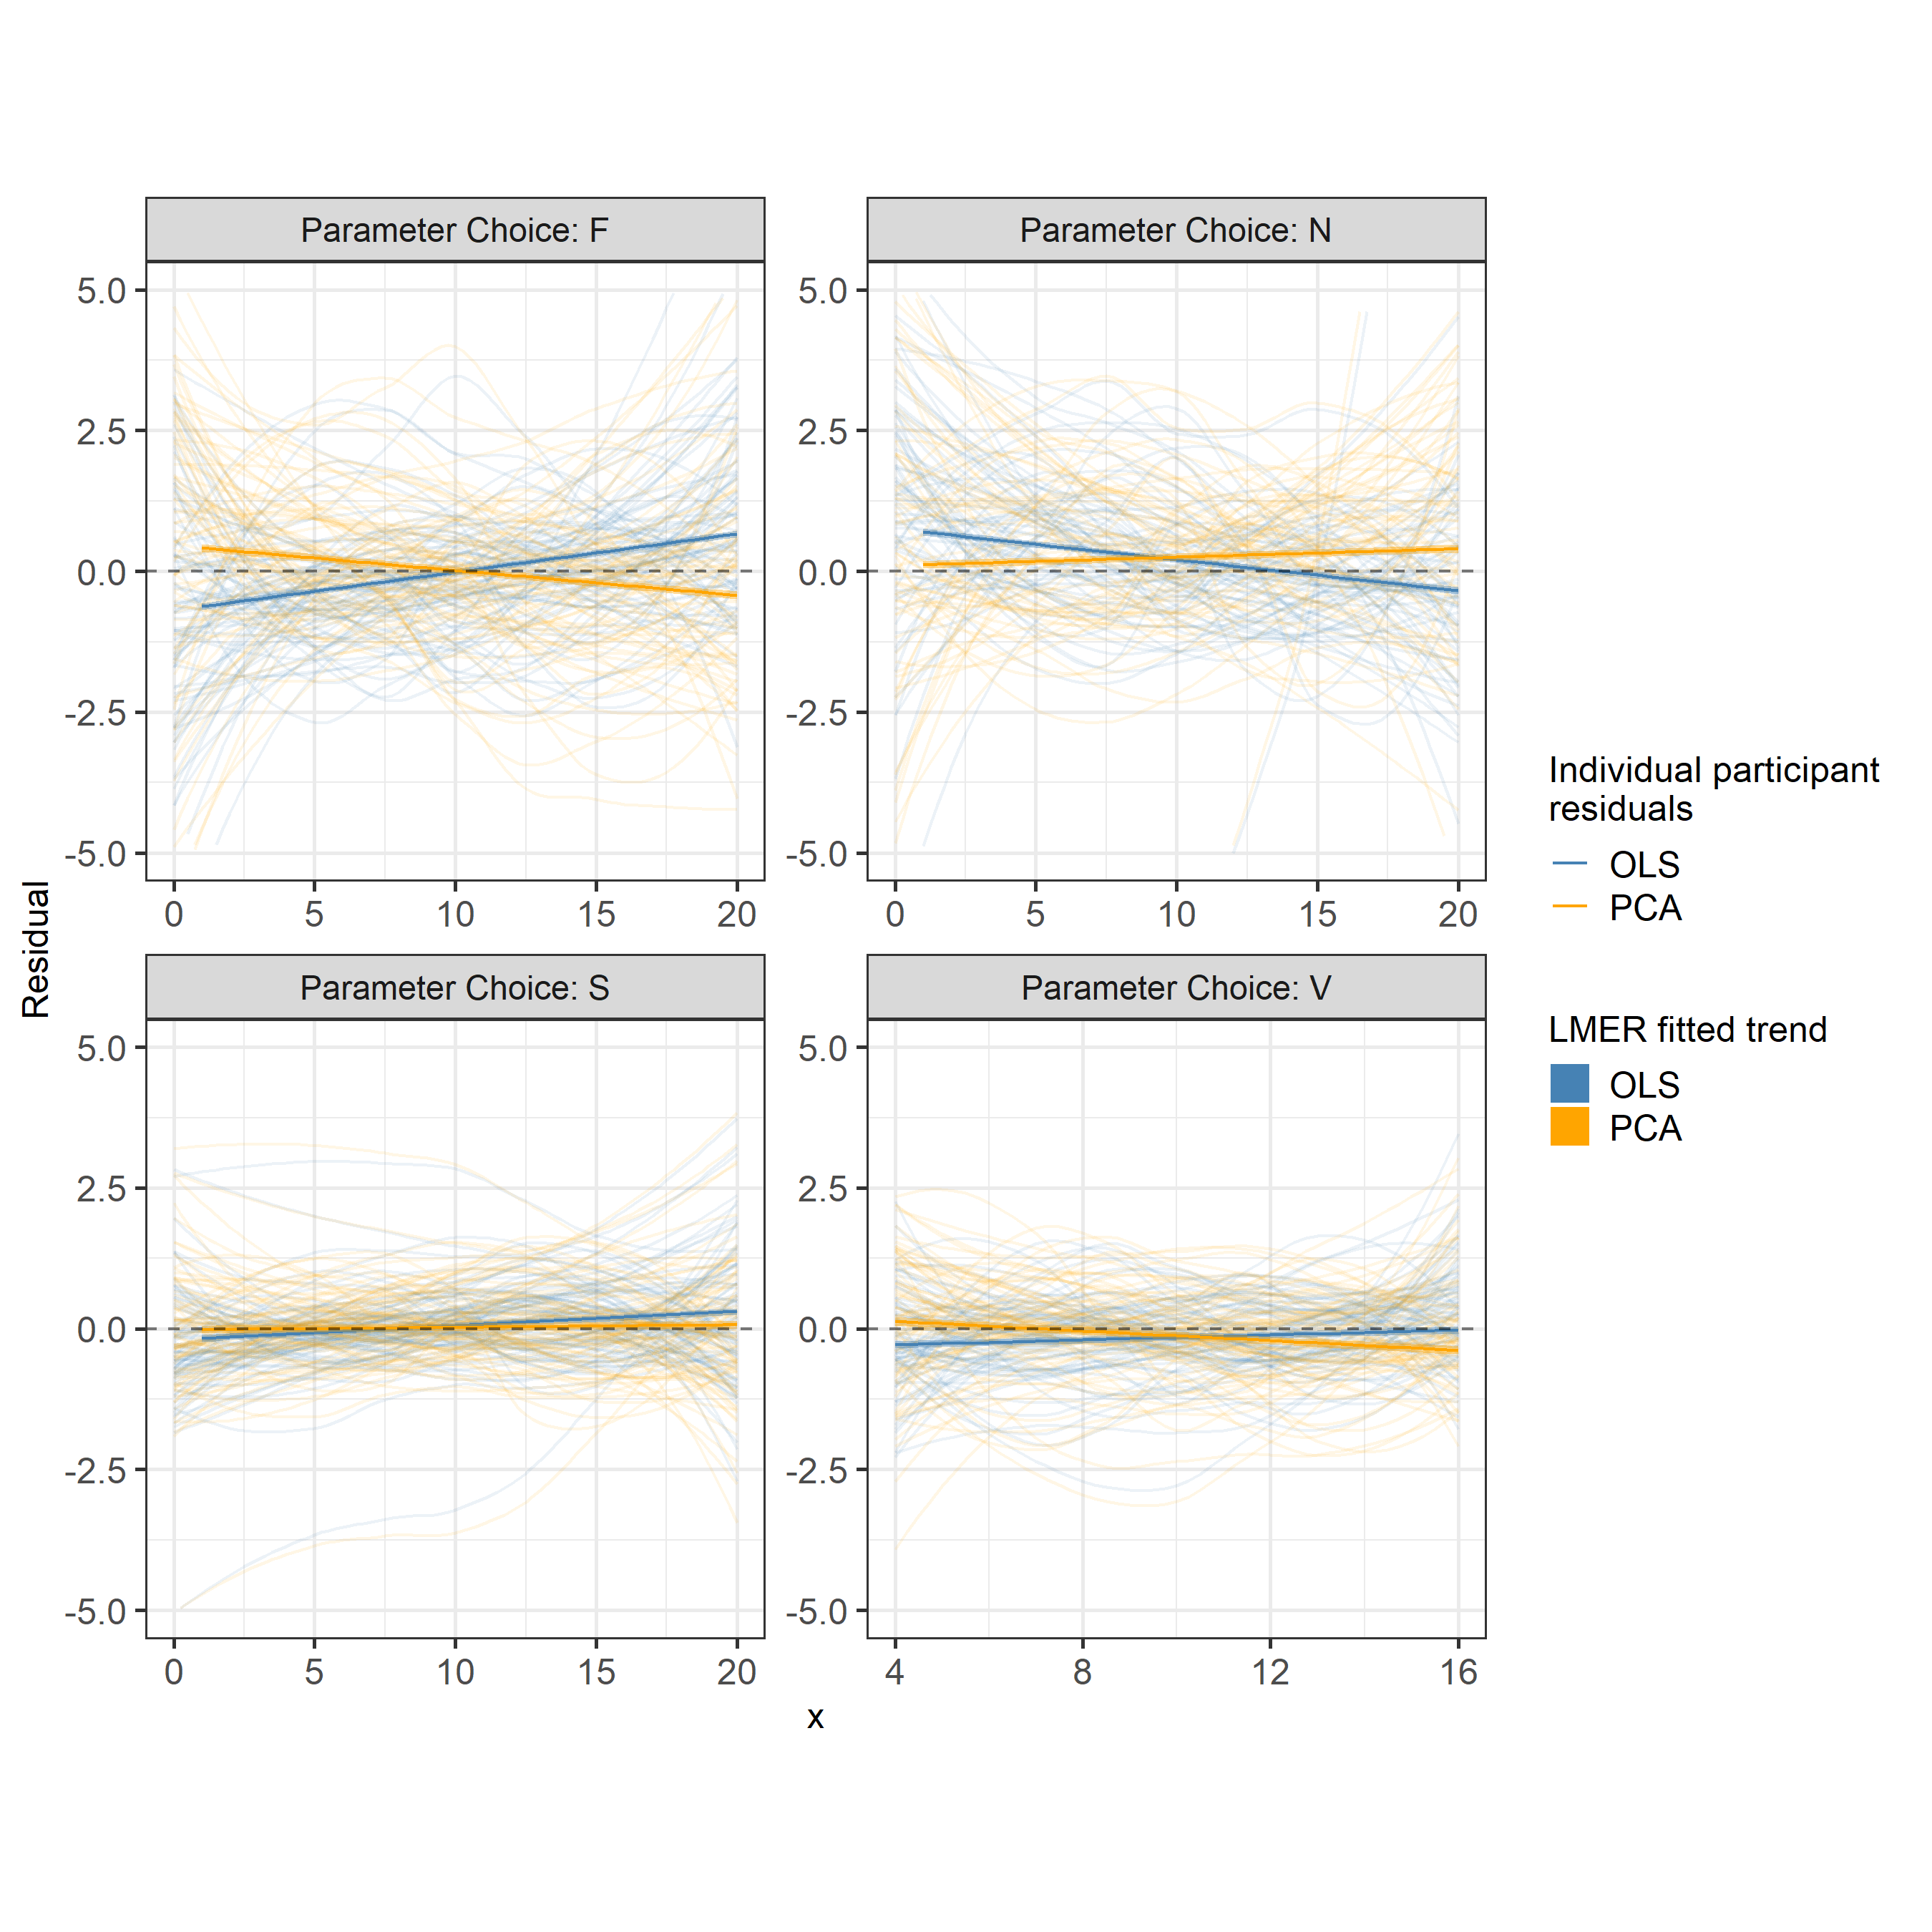
\includegraphics[width=0.9\linewidth,]{thesis_files/figure-latex/eyefitting-lmer-residualplots-1} 

}

\caption{Eye Fitting Straight Lines in the Modern Era LMM results}\label{fig:eyefitting-lmer-residualplots}
\end{figure}

\begin{figure}[tbp]

{\centering 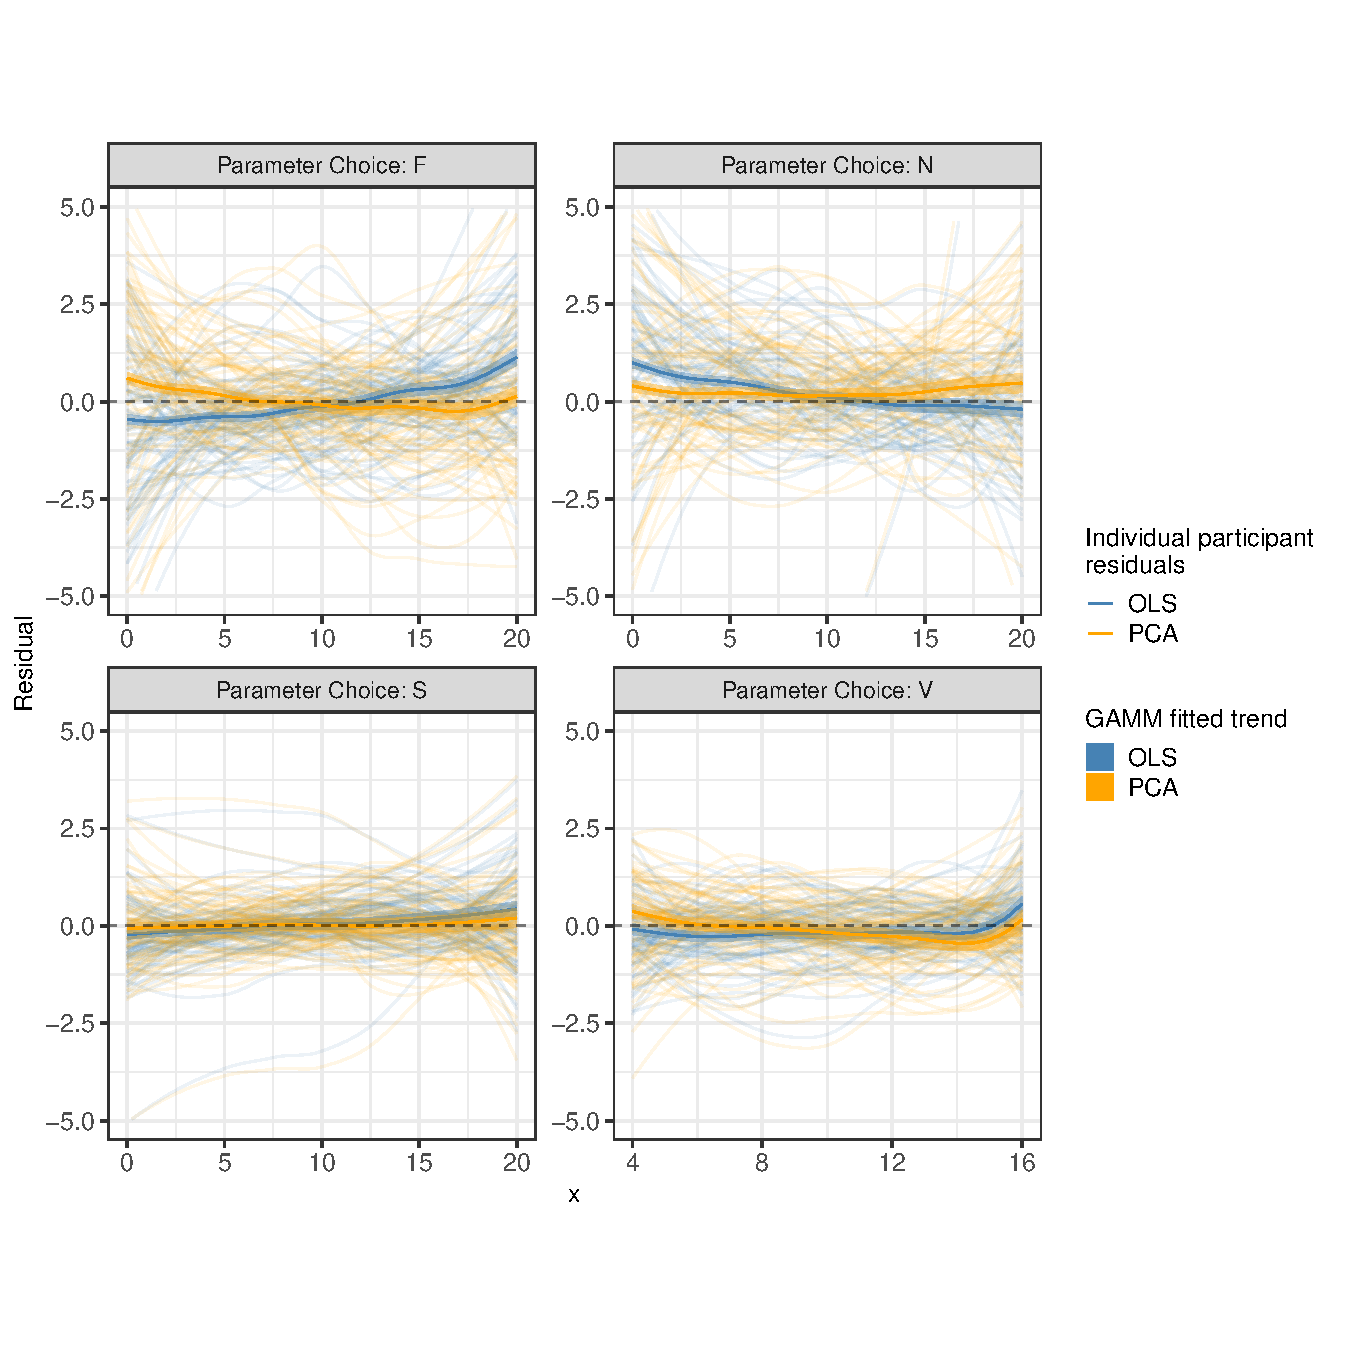
\includegraphics[width=0.9\linewidth,]{thesis_files/figure-latex/eyefitting-gamm-residualplots-1} 

}

\caption{Eye Fitting Straight Lines in the Modern Era GAMM results}\label{fig:eyefitting-gamm-residualplots}
\end{figure}

In addition to fitting trend lines over the residuals between the participant drawn values and fitted values, an OLS sum of squares and PCA sums of squares measure was calculated for each you draw it plot.
Sums of squares between fits were compared using lmer (Bates, Mächler, Bolker, \& Walker, 2015) to run a linear mixed model (LMM) with a log transformation.
Parameter choice, fit, and the interaction between parameter choice and fit were treated as fixed effects with a random participant effect.
Define \(SS_{ijk}\) as the sums of squares for parameter choice \(i = 1,2,3,4\), fit \(j=1,2\), and participant \(k = 1,...,N_{participant}\).
The LMM equation is given by:
\begin{equation}
\log\left(SS_{ijk}\right) = \alpha_i + \beta_j + \alpha\beta_{ij} + p_{j} + \epsilon_{ij}
\end{equation}

\begin{itemize}
\tightlist
\item
  \(\alpha_i\) denotes the effect of the \(i^{th}\) parameter choice
\item
  \(\beta_j\) denotes the effect of the \(j^{th}\) fit
\item
  \(\alpha\beta_{ij}\) denotes the interaction between the parameter choice and fit
\item
  \(p_{j} \sim N(0, \sigma^2_{participant})\) is the random error due to participant variation
\item
  \(\epsilon_{ij} \sim N(0, \sigma^2)\) is the residual error.
\end{itemize}

\cref{fig:eyefitting-ss-oddsratio} displays estimated odds ratios between the OLS fit and PCA fit for each parameter choice.
While there is no significant effect of fit for any parameter choices, there is indication of the trend found previously in the residual regression models.

\begin{figure}[tbp]

{\centering 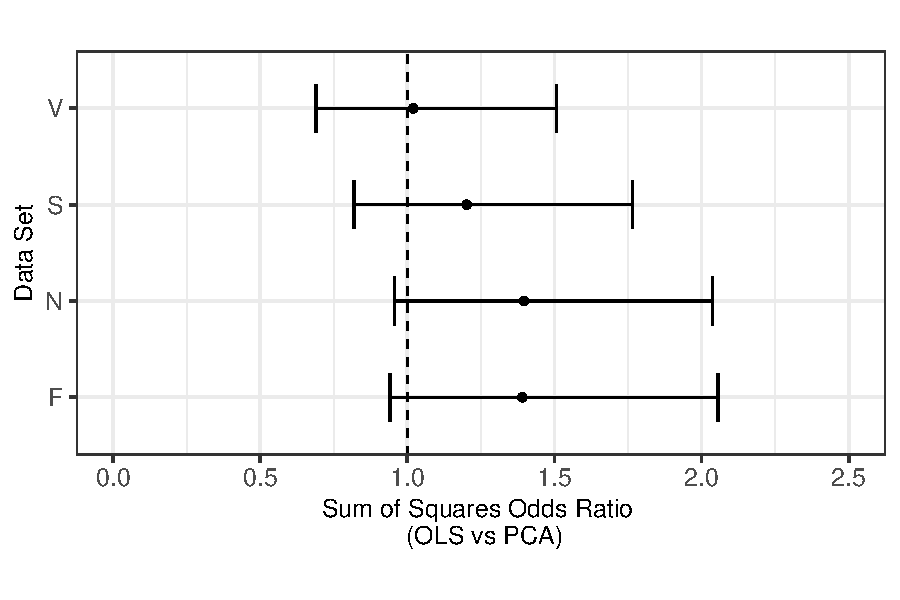
\includegraphics[width=0.75\linewidth,]{thesis_files/figure-latex/eyefitting-ss-oddsratio-1} 

}

\caption{Eye Fitting Straight Lines in the Modern Era Sum of Squares Results}\label{fig:eyefitting-ss-oddsratio}
\end{figure}

\hypertarget{prediction-of-exponential-trends}{%
\section{Prediction of Exponential Trends}\label{prediction-of-exponential-trends}}

The results from the first sub-study validate you draw it as a tool for testing graphics.
This sub-study is designed to test an individual's ability to make predictions for exponentially increasing data on both the log and linear scales, addressesing cognitive understanding of log scales.
Participants are asked to draw a line using their computer mouse through the exponentially increasing trend shown on both the log and linear scale.

\hypertarget{data-generation-2}{%
\subsection{Data Generation}\label{data-generation-2}}

All data processing was conducted in R before being passed to the D3.js source code.
A total of \(N = 30\) points \((x_i, y_i), i = 1,...N\) were generated for \(x\in [x_{min}, x_{max}]\) where \(x\) and \(y\) have an exponential relationship.
Data was simulated based on a one parameter exponential model with multiplicative errors:
\begin{align}
y_i & = e^{\beta x + e_i} \\
\text{with } e_i & \sim N(0, \sigma^2). \nonumber
\end{align}
The parameter, \(\beta\), was selected to reflect the rate of exponential growth with \(e_i\) generated by rejection sampling in order to guarantee the points shown align with that of the fitted line displayed in the initial plot frame.
A nonlinear least squares regression is then fit to the simulated points in order to obtain the best fit line and fitted values in 0.25 increments across the domain, \((x_k, \hat y_{k,NLS}), k = 1, ..., 4\cdot x_{max} +1\).
The data simulation function then outputs a list of point data and line data both indicating the parameter identification, x value, and corresponding simulated or fitted y value.
The data simulation procedure is described in \cref{alg:exponential-prediction-algorithm}.

\begin{algorithm}
  \caption{Prediction of Exponential Trends Data Simulation}\label{exponential-prediction-algorithm}
  \begin{algorithmic}[1]
    \Statex \textbullet~\textbf{Input Parameters:} $\beta$ growth rate; standard deviation from exponential curve $\sigma$; sample size $N = 30$; domain $x_{min}$ and $x_{max}$; fitted value increment $x_{by} = 0.25$.
    \Statex \textbullet~\textbf{Output Parameters:} List of point data and line data each indicating the parameter identification, x value, and corresponding simulated or fitted y value.
    \State Randomly select and jitter N = 30 x-values along the domain, $x_{i=1:N}\in [0, 20]$.
    \State Generate "good" errors, $e_{i = 1:n}$ based on $N(0,\sigma)$ by setting a constraint requiring the mean of the first N/3 errors $< |2\sigma|.$
    \State Simulate point data based on $y_i = e^{\beta x + e_i}$.
    \State Fit the equation $\log(y) = \beta x$ to obtain an estimated starting value for $\beta$. 
    \State Obtain nonlinear least squares regression coefficient, $\hat\beta$, for the simulated point data using the `nls` function in the base stats R package.
    \State Obtain fitted values every 0.25 increment across the domain from the nonlinear least squares regression $\hat y_{m,NLS} = e^{\hat\beta_{NLS} x_m}$.
    \State Output data list of point data and line data each indicating the parameter identification, x value, and corresponding simulated or fitted y value.
  \end{algorithmic}
\end{algorithm}

Model equation parameter, \(\beta\), was selected to reflect two exponential growth rates (low: \(\beta = 0.10, \sigma = 0.09\) and high: \(\beta = 0.23, \sigma = 0.25\)) as determined by visual inspection with growth rate parameter selection from the lineup study in \protect\hyperlink{lineups-parameter-selection}{Chapter 2} used as a starting point.
Each growth rate parameter was used to simulate data across a domain of 0 to 20.
The 2 simulated data sets (low and high exponential growth rates) were then shown 4 times each by truncating the points shown at both 50\% and 75\% of the domain as well as on both the log and linear scales for a total of 8 interactive plots reflecting a 2 x 2 x 2 factorial treatment design.
\protect\hyperlink{exponential-prediction-plots}{Appendix B} displays visual examples of all 8 interactive plots.
Within the interactive plot code, the aspect ratio defining the x to y axis ratio was set to 1 with a y range buffer of 50\% on the lower limit and 200\% on the upper limit to allow for users to draw outside the data set range.
The linear scale option was set to true or false reflecting the linear and log scale display choices respectively with the user line start draw point set to 50\% of the domain at \(x = 10\).

\hypertarget{results-2}{%
\subsection{Results}\label{results-2}}

A Loess smoother was fit to each user line to allow for visual inspection.
For each participant \(l = 1,...N_{participant}\), the final data set used for analysis contains \(x_{ijkm}, y_{ijkm,drawn}, \hat y_{ijkm,loess}\), and \(\hat y_{ijkm,NLS}\) for growth rate \(i = 1,2\), points truncated \(j = 1,2\), scale \(k = 1,2\) and \(x_{m}\) value \(m = 1, ...,81\).
\cref{fig:exponential-yloess-spaghetti-plot} displays spaghetti plots for each of the 8 treatment combinations.
The spaghetti plot with a high growth rate suggests participants underestimated the exponential trend when asked to draw a trend line on the linear scale compared to when asked to draw a trend line on the log scale.
In particular, this suggestion is most noticeable when points are truncated at 50\% with the underestimation begining at a later \(x\) value when points are truncated at 75\%.

\begin{figure}[tbp]

{\centering 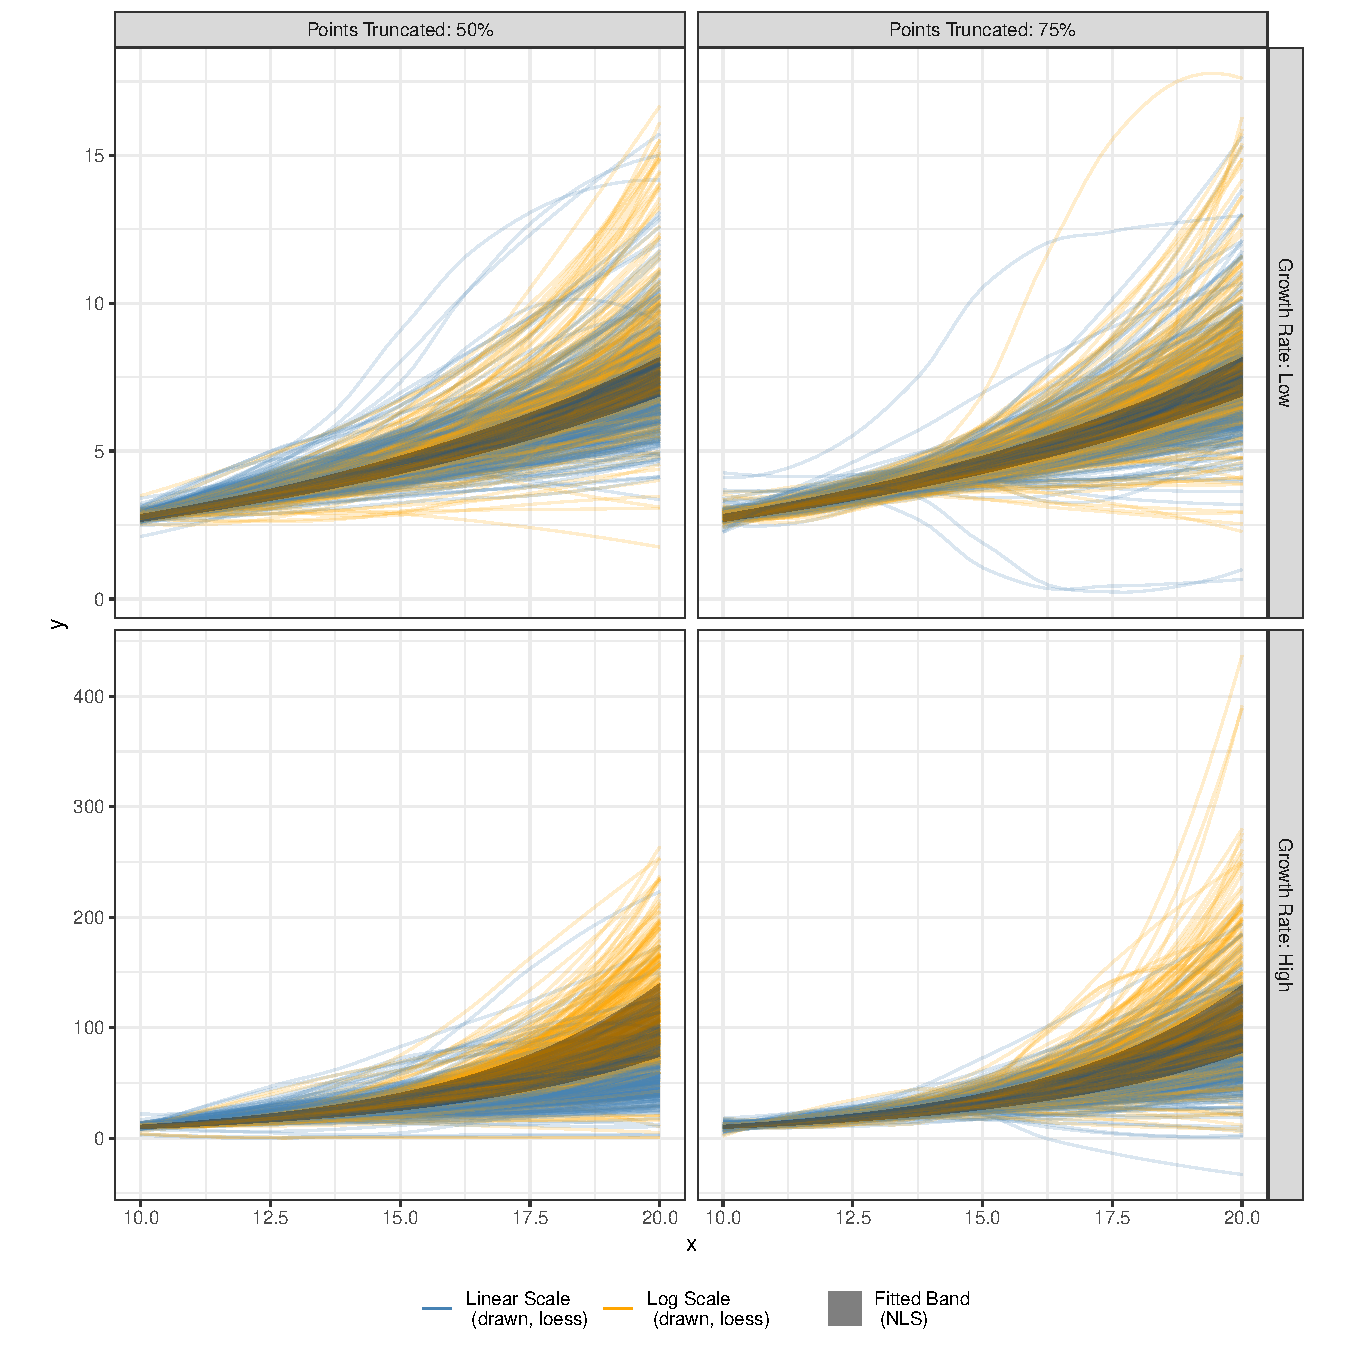
\includegraphics[width=0.9\linewidth,]{thesis_files/figure-latex/exponential-yloess-spaghetti-plot-1} 

}

\caption{Exponential Prediction Spaghetti Plot}\label{fig:exponential-yloess-spaghetti-plot}
\end{figure}

Allowing for flexibility, the bam function in the mgcv package (S. N. Wood, 2003, 2004, 2011; S. N. Wood, 2017; S. N. Wood, N., Pya, \& Saefken, 2016) is used to fit a GAMM to estimate trends of vertical residuals from the participant drawn line in relation to the NLS fitted values (\(e_{ijklm,NLS} = y_{ijklm,drawn} - \hat y_{ijklm,NLS}\)) across the domain of \(x\).
The combination between growth rate, point truncation, and scale was treated as a fixed effect with no estimated intercept and a separate smoothing spline for \(x\) was estimated for each treatment combination.
A random participant effect accounting for variation due to participant and a random spline for each participant accounted for variation in spline for each participant.
The GAMM equation for residuals is given by:
\begin{equation}
y_{ijklm,drawn} - y_{ijklm,NLS} = e_{ijklm,nls} = \tau_{ijk} + s_{ijk}(x_{ijkm}) + p_{l} + s_{m}(x_{ijklm})
\end{equation}
\noindent where

\begin{itemize}
\tightlist
\item
  \(\tau_{ijk}\) is the intercept for the \(i^{th}\) growth rate, \(j^{th}\) point truncation, and \(k^{th}\) scale treatment combination
\item
  \(s_{ijk}\) is the smoothing spline for the \(ijk^{th}\) treatment combination
\item
  \(p_{m} \sim N(0, \sigma^2_{participant})\) is the error due to participant variation
\item
  \(s_{m}\) is the random smoothing spline for each participant.
\end{itemize}

\cref{fig:exponential-prediction-gamm-preds} show the estimated trends of residuals (vertical deviation of participant drawn points from NLS fitted points) as modeled by a GAMM.
Examining the plots, the estimated trends of residuals of trends drawn on the linear scale (blue) appear to deviate from the \(y=0\) horizontal (dashed) line indicating underestimation of exponential growth.
In comparisons, the estimated trends of trends residuals drawn on the log scale (orange) follow closely to the \(y=0\) horizontal (dashed) line implying exponential trends predicted on the log scale are more accurate than those predicted on the linear scale.
In particular, this trend is more prominent in high exponential growth rates where underestimation becomes prominent after the aid of points is removed.

\begin{figure}[tbp]

{\centering 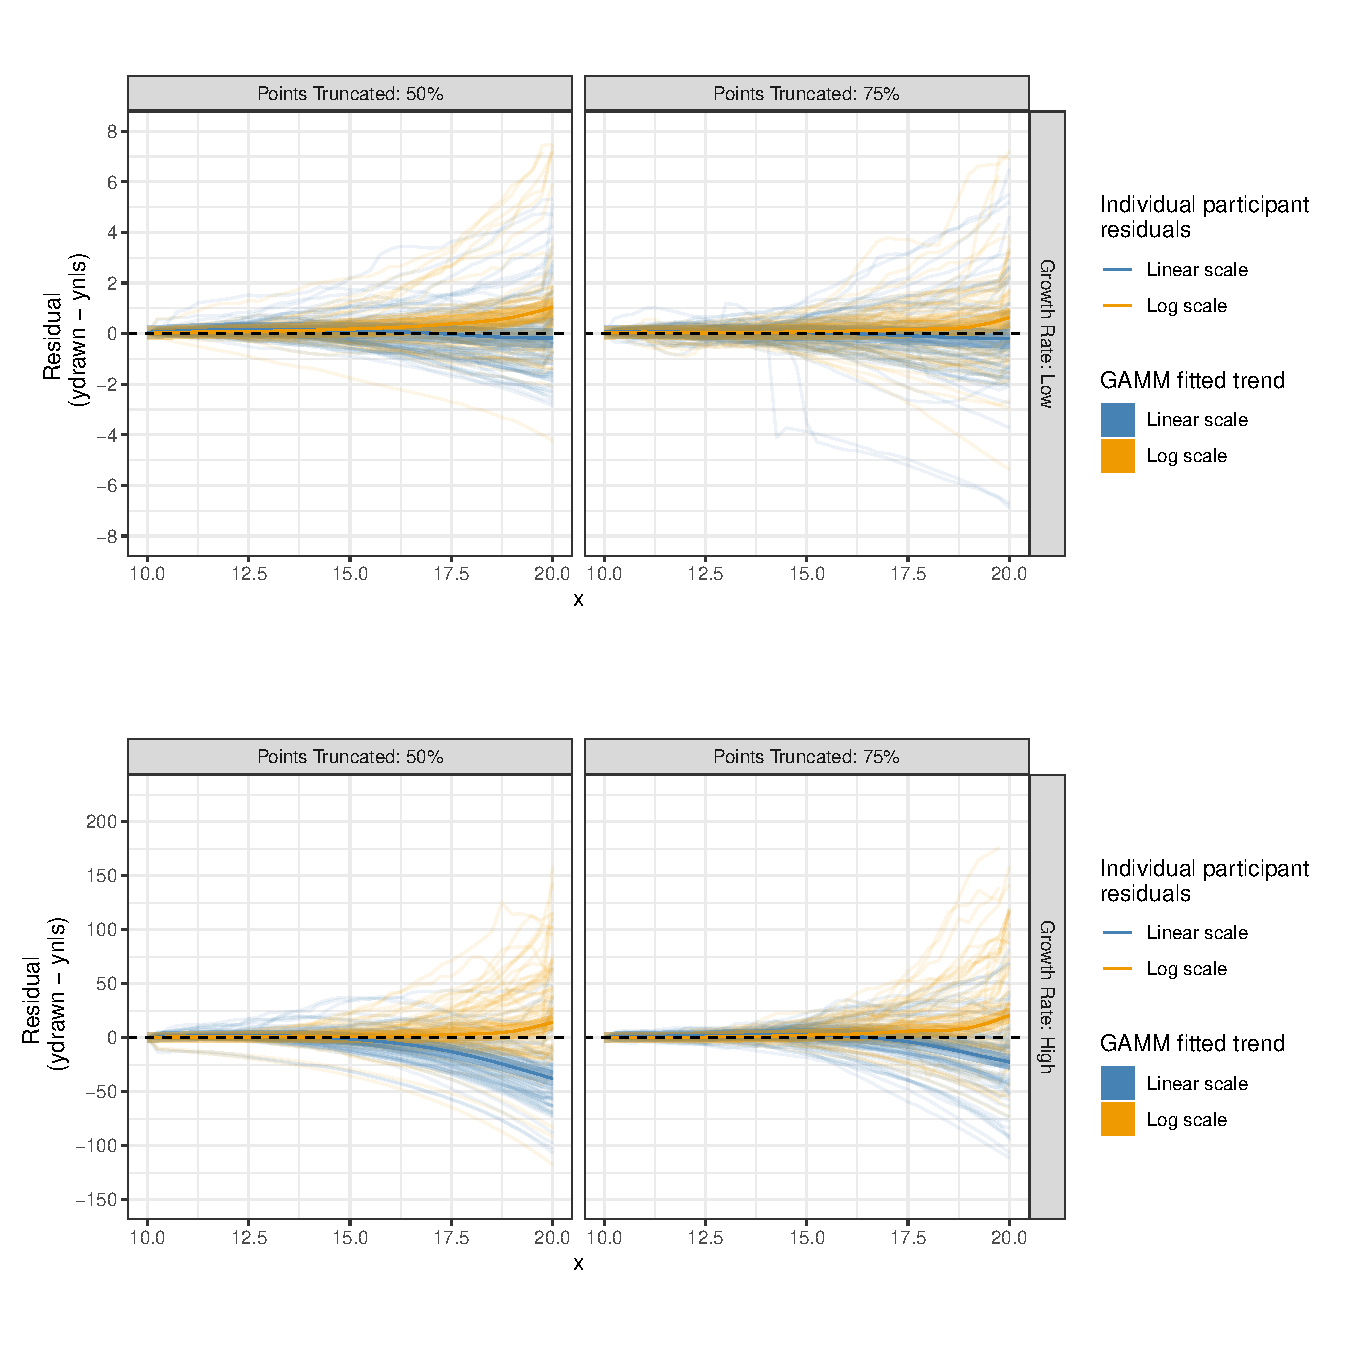
\includegraphics[width=0.9\linewidth,]{thesis_files/figure-latex/exponential-prediction-gamm-preds-1} 

}

\caption{Exponential Prediction GAMM Results}\label{fig:exponential-prediction-gamm-preds}
\end{figure}

\hypertarget{discussion-and-conclusion-1}{%
\section{Discussion and Conclusion}\label{discussion-and-conclusion-1}}

The intent of this chapter was to establish you draw it as a tool for testing graphics then use this tool to determine the cognitive implications of displaying data on the log scale.
Eye Fitting Straight Lines in the Modern Era replicated the results found in Mosteller, Siegel, Trapido, \& Youtz (1981).
When shown points following a linear trend, participants tended to fit the slope of the first principal component over the slope of the least squares regression line.
This trend was most prominent when shown data simulated with larger variances.
The reproducibility of these results serve as evidence of the reliability of the you draw it method.

In Prediction of Exponential Trends, the you draw it method was used to test an individual's ability to make predictions for exponentially increasing data.
Results indicate that underestimation of exponential growth occurs when participants were asked to draw trend lines on the linear scale and that there was an improvement in accuracy when trends were drawn on the log scale.
This phenomena is strongly supported for high exponential growth rates.
Improvement in predictions are made when points along the exponential trend are shown as indicated by the discrepancy in results for treatments with points truncated at 50\% compared to 75\% of the domain.

The results of this study suggest that there are cognitive advantages to log scales when making predictions of exponential trends.
Improvement in predictions were made for trends with high exponential growth rates when participants were asked to draw a trend line on the log scale compared to the linear scale.
Further investigation is necessary to determine the implications of using log scales when translating exponential graphs to numerical values.

\appendix

\hypertarget{youdrawit-with-shiny}{%
\chapter{You Draw It Setup with Shiny}\label{youdrawit-with-shiny}}

Interactive plots for the you draw it study were created using the r2d3 package and integrating D3 source code with an R shiny application.
In this section I outline the process of constructing interactive plots with D3.js code and R shiny.

\cref{fig:r2d3-shiny-flowchart}

\begin{figure}[tbp]

{\centering 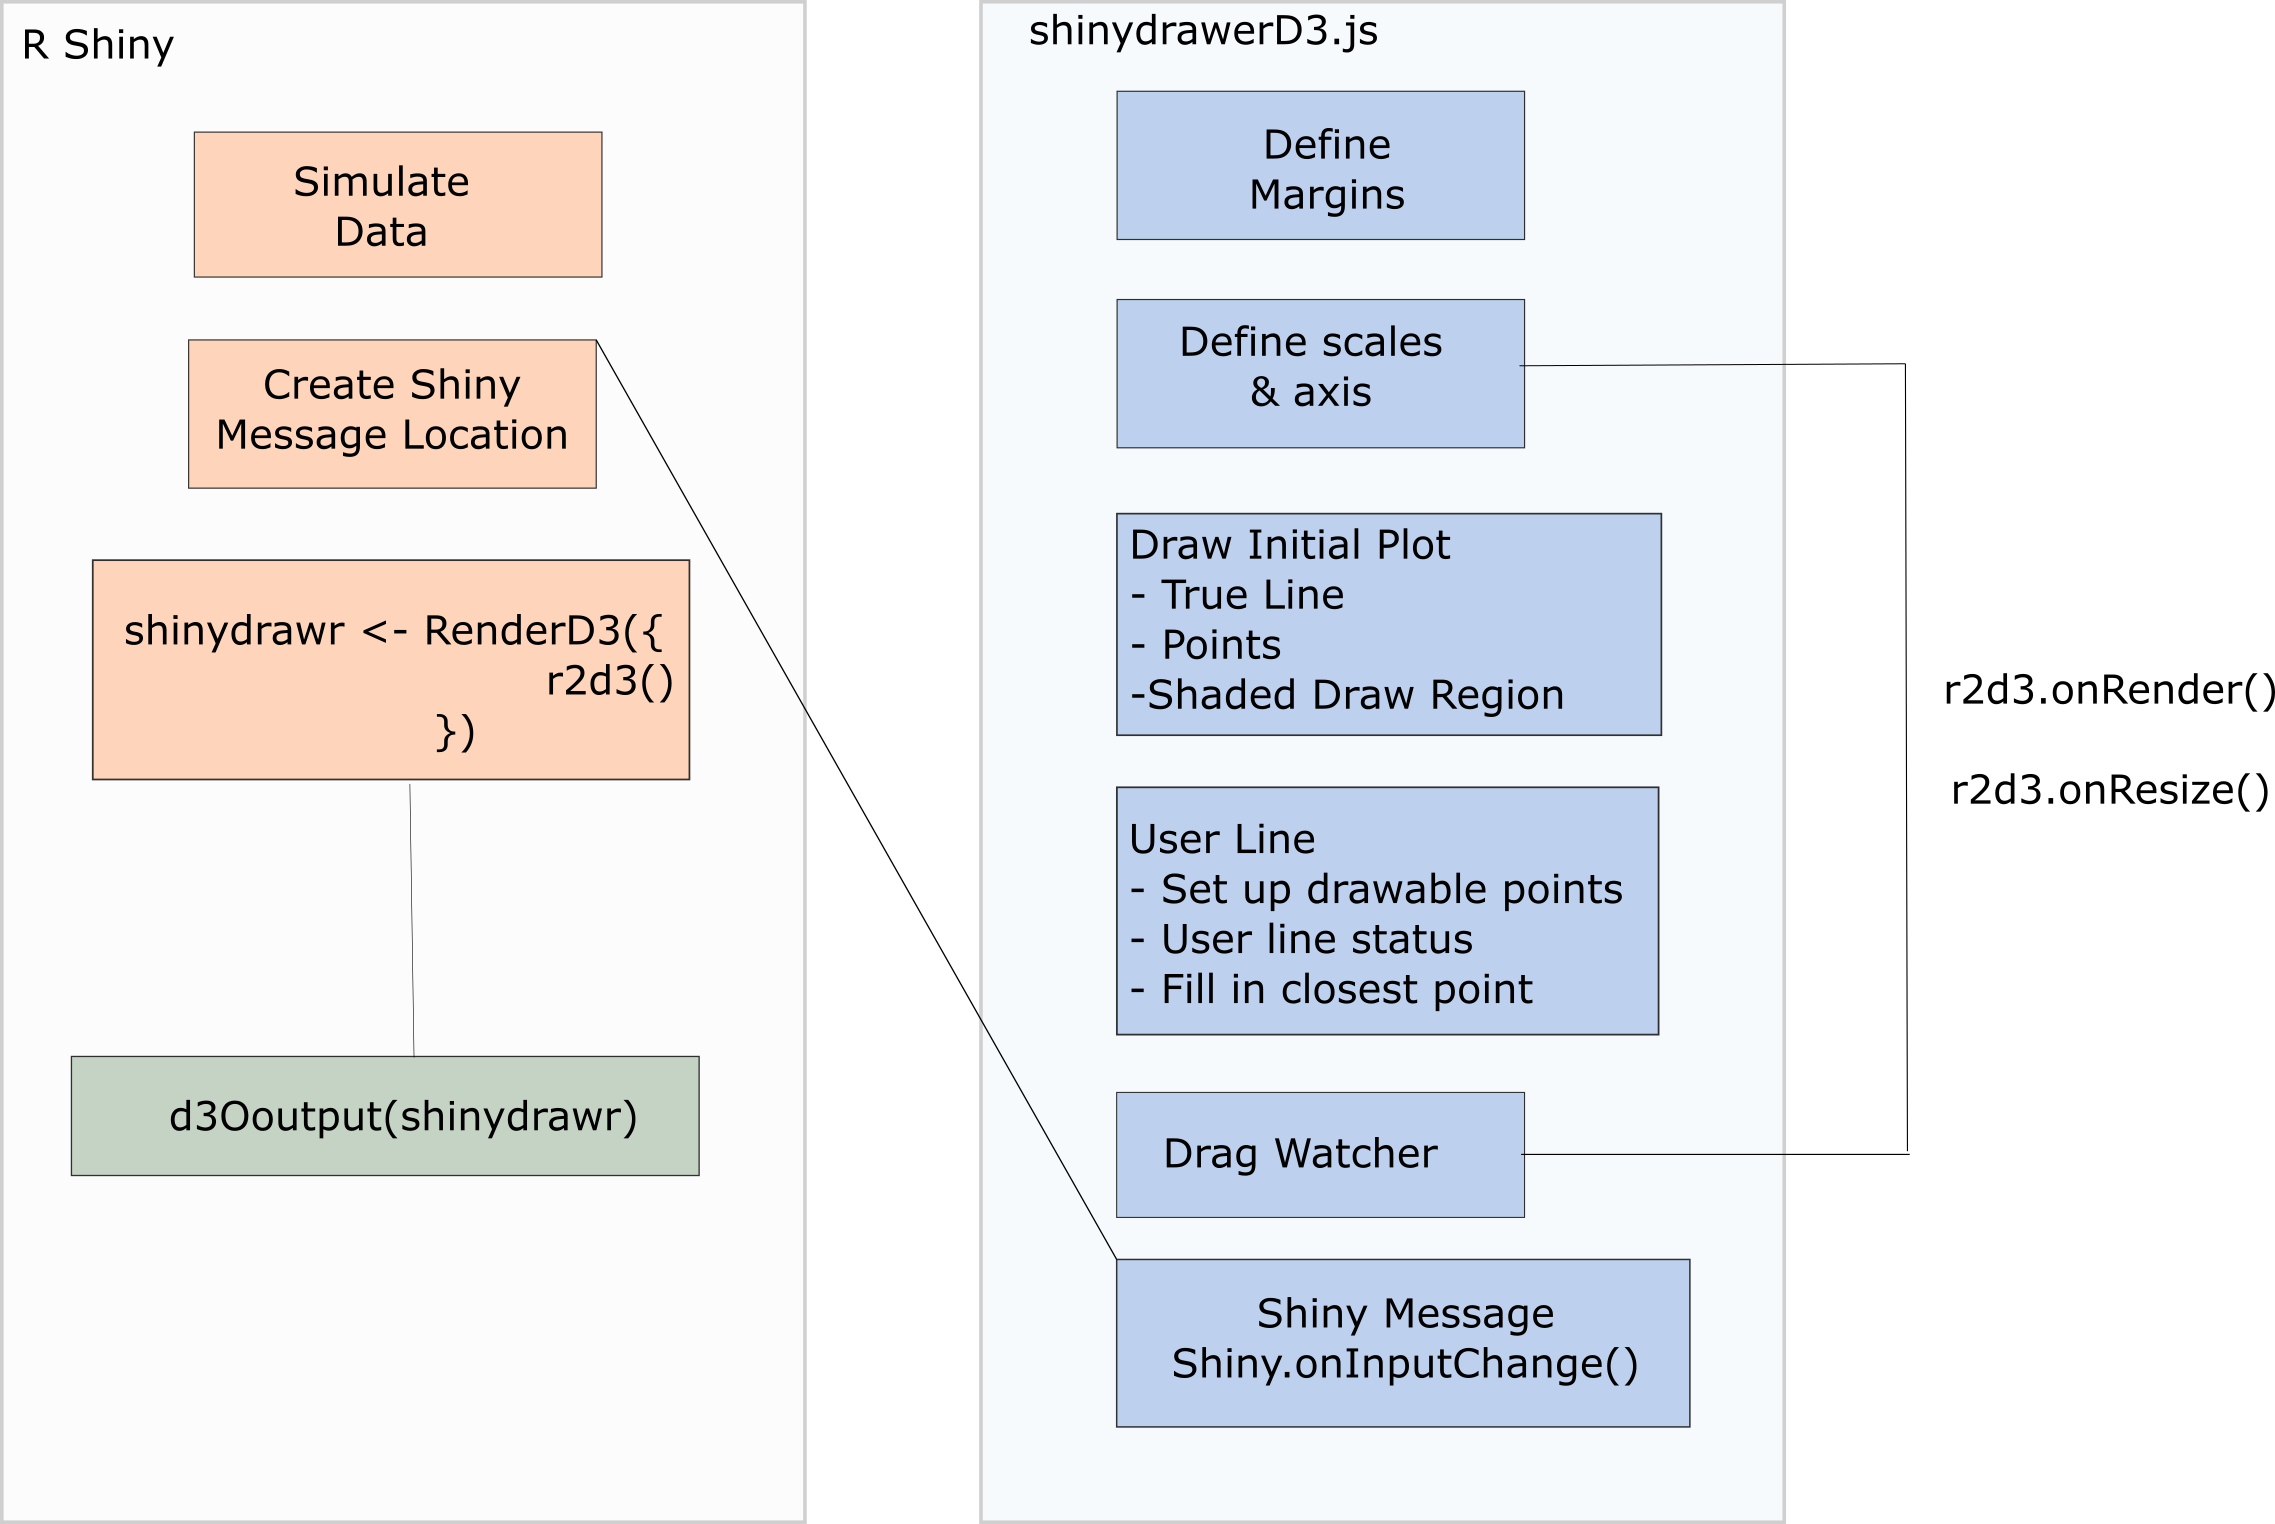
\includegraphics[width=0.8\linewidth,]{images/r2d3+shiny-inkscape} 

}

\caption{Interactive plot development}\label{fig:r2d3-shiny-flowchart}
\end{figure}

\hypertarget{exponential-prediction-plots}{%
\chapter{Exponential Prediction Interactive Plots}\label{exponential-prediction-plots}}

The figures below illustrate the 8 interactive plots used to test exponential prediction.
Two data sets were simulated with low and high exponential growth rates and shown four times each by truncating the points shown at both 50\% and 75\% of the domain as well as on both the log and linear scales following a 2 x 2 x 2 factorial treatment design.

\begin{figure}[tbp]

{\centering 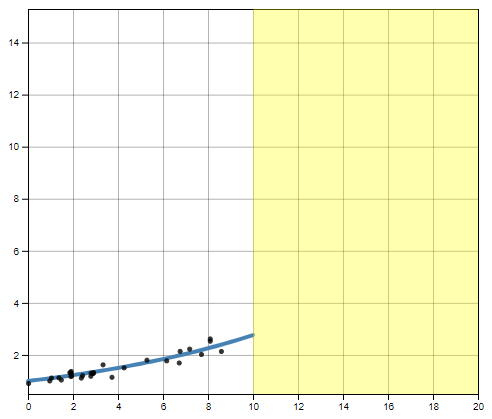
\includegraphics[width=0.65\linewidth,]{images/low-10-linear} 

}

\caption{Exponential Prediction: low growth rate, points truncated at 50\%, linear scale}\label{fig:low-10-linear}
\end{figure}

\begin{figure}[tbp]

{\centering 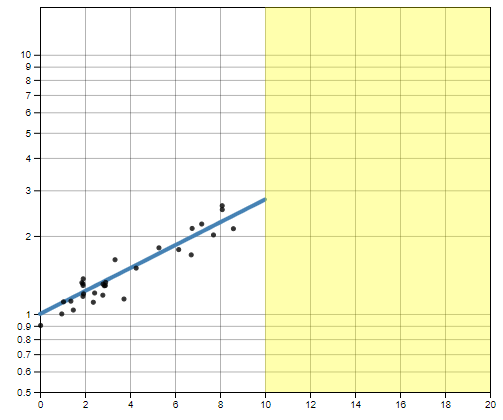
\includegraphics[width=0.65\linewidth,]{images/low-10-log} 

}

\caption{Exponential Prediction: low growth rate, points truncated at 50\%, log scale}\label{fig:low-10-log}
\end{figure}

\begin{figure}[tbp]

{\centering 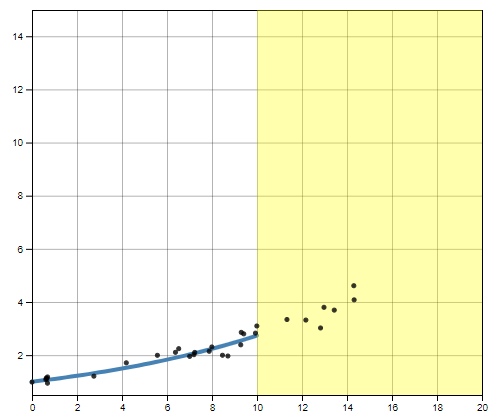
\includegraphics[width=0.65\linewidth,]{images/low-15-linear} 

}

\caption{Exponential Prediction: low growth rate, points truncated at 75\%, linear scale}\label{fig:low-15-linear}
\end{figure}

\begin{figure}[tbp]

{\centering 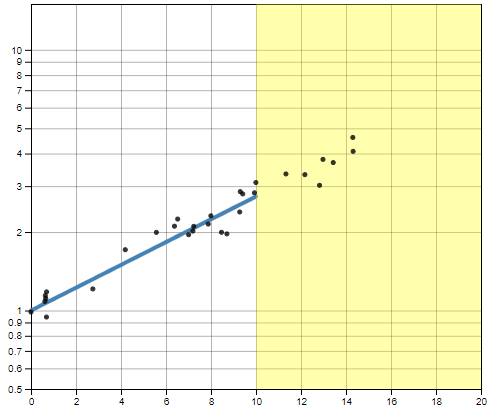
\includegraphics[width=0.65\linewidth,]{images/low-15-log} 

}

\caption{Exponential Prediction: low growth rate, points truncated at 75\%, log scale}\label{fig:low-15-log}
\end{figure}

\begin{figure}[tbp]

{\centering 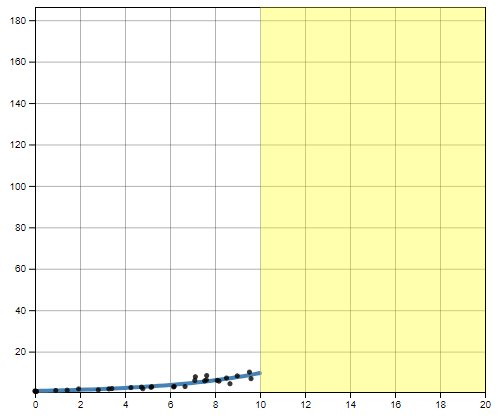
\includegraphics[width=0.65\linewidth,]{images/high-10-linear} 

}

\caption{Exponential Prediction: high growth rate, points truncated at 50\%, linear scale}\label{fig:high-10-linear}
\end{figure}

\begin{figure}[tbp]

{\centering 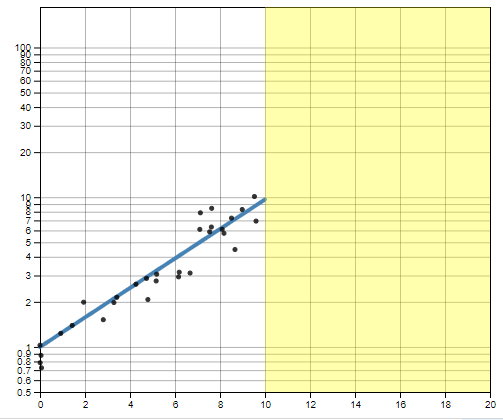
\includegraphics[width=0.65\linewidth,]{images/high-10-log} 

}

\caption{Exponential Prediction: high growth rate, points truncated at 50\%, log scale}\label{fig:high-10-log}
\end{figure}

\begin{figure}[tbp]

{\centering 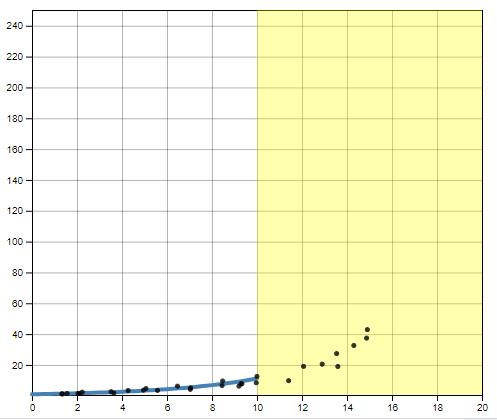
\includegraphics[width=0.65\linewidth,]{images/high-15-linear} 

}

\caption{Exponential Prediction: high growth rate, points truncated at 75\%, linear scale}\label{fig:high-15-linear}
\end{figure}

\begin{figure}[tbp]

{\centering 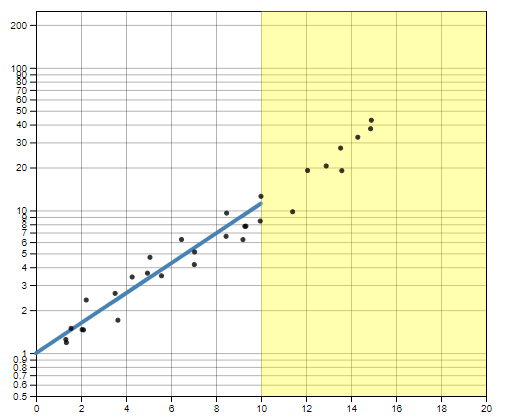
\includegraphics[width=0.65\linewidth,]{images/high-15-log} 

}

\caption{Exponential Prediction: high growth rate, points truncated at 75\%, log scale}\label{fig:high-15-log}
\end{figure}

\backmatter

\hypertarget{references}{%
\chapter*{References}\label{references}}
\addcontentsline{toc}{chapter}{References}

\noindent

\setlength{\parindent}{-0.20in}
\setlength{\leftskip}{0.20in}
\setlength{\parskip}{8pt}

\hypertarget{refs}{}
\begin{CSLReferences}{1}{0}
\leavevmode\hypertarget{ref-NYTimes_presidential_forecast}{}%
Aisch, G., Cohn, N., Cox, A., Katz, J., Pearce, A., \& Quealy, K. (2016). Live presidential forecast. \emph{The New York Times}. The New York Times. Retrieved from \url{https://www.nytimes.com/elections/2016/forecast/president}

\leavevmode\hypertarget{ref-aisch_cox_quealy_2015}{}%
Aisch, G., Cox, A., \& Quealy, K. (2015, May). You draw it: How family income predicts children's college chances. \emph{The New York Times}. The New York Times. Retrieved from \url{https://www.nytimes.com/interactive/2015/05/28/upshot/you-draw-it-how-family-income-affects-childrens-college-chances.html}

\leavevmode\hypertarget{ref-amer2005bias}{}%
Amer, T. (2005). Bias due to visual illusion in the graphical presentation of accounting information. \emph{Journal of Information Systems}, \emph{19}(1), 1--18.

\leavevmode\hypertarget{ref-NYTrememberinglives}{}%
Barry, D., Buchanan, L., Cargill, C., Daniel, A., Delaquérière, A., Gamio, L., \ldots{} al., et. (2020, May). Remembering the 100,000 lives lost to coronavirus in america. \emph{The New York Times}. The New York Times. Retrieved from \url{https://www.nytimes.com/interactive/2020/05/24/us/us-coronavirus-deaths-100000.html}

\leavevmode\hypertarget{ref-lme4}{}%
Bates, D., Mächler, M., Bolker, B., \& Walker, S. (2015). Fitting linear mixed-effects models using {lme4}. \emph{Journal of Statistical Software}, \emph{67}(1), 1--48. http://doi.org/\href{https://doi.org/10.18637/jss.v067.i01}{10.18637/jss.v067.i01}

\leavevmode\hypertarget{ref-bavel_using_2020}{}%
Bavel, J. J. V., Baicker, K., Boggio, P. S., Capraro, V., Cichocka, A., Cikara, M., \ldots{} Willer, R. (2020). Using social and behavioural science to support {COVID}-19 pandemic response. \emph{Nature Human Behaviour}, \emph{4}(5), 460--471. http://doi.org/\href{https://doi.org/10.1038/s41562-020-0884-z}{10.1038/s41562-020-0884-z}

\leavevmode\hypertarget{ref-vonbergmann_2021}{}%
Bergmann, J. von. (2021, March). \emph{mountainMath}. GitHub. Retrieved from \url{https://github.com/mountainMath/xkcd_exponential}

\leavevmode\hypertarget{ref-best_perception_2007}{}%
Best, L. A., Smith, L. D., \& Stubbs, D. A. (2007). Perception of {Linear} and {Nonlinear} {Trends}: {Using} {Slope} and {Curvature} {Information} to {Make} {Trend} {Discriminations}. \emph{Perceptual and Motor Skills}, \emph{104}(3), 707--721. http://doi.org/\href{https://doi.org/10.2466/pms.104.3.707-721}{10.2466/pms.104.3.707-721}

\leavevmode\hypertarget{ref-broersma1985graphical}{}%
Broersma, H., \& Molenaar, I. (1985). Graphical perception of distributional aspects of data. \emph{Computational Statistics Quarterly}, \emph{2}(1), 53--72.

\leavevmode\hypertarget{ref-buchanan_park_pearce_2017}{}%
Buchanan, L., Park, H., \& Pearce, A. (2017, January). You draw it: What got better or worse during obama's presidency. \emph{The New York Times}. The New York Times. Retrieved from \url{https://www.nytimes.com/interactive/2017/01/15/us/politics/you-draw-obama-legacy.html}

\leavevmode\hypertarget{ref-buja_statistical_2009}{}%
Buja, A., Cook, D., Hofmann, H., Lawrence, M., Lee, E.-K., Swayne, D. F., \& Wickham, H. (2009). Statistical inference for exploratory data analysis and model diagnostics. \emph{Philosophical Transactions of the Royal Society A: Mathematical, Physical and Engineering Sciences}, \emph{367}(1906), 4361--4383. http://doi.org/\href{https://doi.org/10.1098/rsta.2009.0120}{10.1098/rsta.2009.0120}

\leavevmode\hypertarget{ref-burnmurdoch_2020}{}%
Burn-Murdoch, J., Nevitt, C., Tilford, C., Rininsland, A., Kao, J. S., Elliott, O., \ldots{} Stabe, M. (2020). Coronavirus tracked: Has the epidemic peaked near you? \emph{Coronavirus chart: see how your country compares}. Financial Times. Retrieved from \url{https://ig.ft.com/coronavirus-chart/?areas=eur}

\leavevmode\hypertarget{ref-carlson2010psychology}{}%
Carlson, N. R. (2010). \emph{Psychology: The science of behaviour}. Pearson Education.

\leavevmode\hypertarget{ref-chandar2012graph}{}%
Chandar, N., Collier, D., \& Miranti, P. (2012). Graph standardization and management accounting at AT\&t during the 1920s. \emph{Accounting History}, \emph{17}(1), 35--62.

\leavevmode\hypertarget{ref-cleveland_graphical_1984}{}%
Cleveland, W. S., \& McGill, R. (1984). Graphical {Perception}: {Theory}, {Experimentation}, and {Application} to the {Development} of {Graphical} {Methods}. Retrieved from \url{http://euclid.psych.yorku.ca/www/psy6135/papers/ClevelandMcGill1984.pdf}

\leavevmode\hypertarget{ref-cleveland_graphical_1985}{}%
Cleveland, W. S., \& McGill, R. (1985). Graphical {Perception} and {Graphical} {Methods} for {Analyzing} {Scientific} {Data}. \emph{Science, New Series}, \emph{229}(4716), 828--833. Retrieved from \url{http://www.jstor.org/stable/1695272}

\leavevmode\hypertarget{ref-croxton1932graphic}{}%
Croxton, F. E., \& Stein, H. (1932). Graphic comparisons by bars, squares, circles, and cubes. \emph{Journal of the American Statistical Association}, \emph{27}(177), 54--60.

\leavevmode\hypertarget{ref-croxton1927bar}{}%
Croxton, F. E., \& Stryker, R. E. (1927). Bar charts versus circle diagrams. \emph{Journal of the American Statistical Association}, \emph{22}(160), 473--482.

\leavevmode\hypertarget{ref-dehaene2008log}{}%
Dehaene, S., Izard, V., Spelke, E., \& Pica, P. (2008). Log or linear? Distinct intuitions of the number scale in western and amazonian indigene cultures. \emph{Science}, \emph{320}(5880), 1217--1220.

\leavevmode\hypertarget{ref-dunn1988framed}{}%
Dunn, R. (1988). Framed rectangle charts or statistical maps with shading: An experiment in graphical perception. \emph{The American Statistician}, \emph{42}(2), 123--129.

\leavevmode\hypertarget{ref-eells1926relative}{}%
Eells, W. C. (1926). The relative merits of circles and bars for representing component parts. \emph{Journal of the American Statistical Association}, \emph{21}(154), 119--132.

\leavevmode\hypertarget{ref-fagen-ulmschneider_2020}{}%
Fagen-Ulmschneider, W. (2020). 91-DIVOC. \emph{An interactive visualization of COVID-19}. University of Illinois. Retrieved from \url{https://91-divoc.com/pages/covid-visualization/}

\leavevmode\hypertarget{ref-fechner1860elemente}{}%
Fechner, G. T. (1860). \emph{Elemente der psychophysik} (Vol. 2). Breitkopf u. H{ä}rtel.

\leavevmode\hypertarget{ref-finney_subjective_1951}{}%
Finney, D. J. (1951). Subjective {Judgment} in {Statistical} {Analysis}: {An} {Experimental} {Study}. \emph{Journal of the Royal Statistical Society. Series B (Methodological)}, \emph{13}(2), 284--297. Retrieved from \url{https://www.jstor.org/stable/2984070}

\leavevmode\hypertarget{ref-furmanski2000oblique}{}%
Furmanski, C. S., \& Engel, S. A. (2000). An oblique effect in human primary visual cortex. \emph{Nature Neuroscience}, \emph{3}(6), 535--536.

\leavevmode\hypertarget{ref-goldstein_sensation_2017}{}%
Goldstein, E. B., \& Brockmole, J. R. (2017). Sensation and {Perception}, 480.

\leavevmode\hypertarget{ref-gordon_statistician_2015}{}%
Gordon, I., \& Finch, S. (2015). Statistician {Heal} {Thyself}: {Have} {We} {Lost} the {Plot}? \emph{Journal of Computational and Graphical Statistics}, \emph{24}(4), 1210--1229. http://doi.org/\href{https://doi.org/10.1080/10618600.2014.989324}{10.1080/10618600.2014.989324}

\leavevmode\hypertarget{ref-gouretski2007much}{}%
Gouretski, V., \& Koltermann, K. P. (2007). How much is the ocean really warming? \emph{Geophysical Research Letters}, \emph{34}(1).

\leavevmode\hypertarget{ref-green2009personal}{}%
Green, T. M., \& Fisher, B. (2009). The personal equation of complex individual cognition during visual interface interaction. In \emph{Workshop on human-computer interaction and visualization} (pp. 38--57). Springer.

\leavevmode\hypertarget{ref-haemer_presentation_1949}{}%
Haemer, K. W., \& Kelley, T. L. (1949). Presentation {Problems}: {Suiting} the {Chart} to the {Audience}: {Common} {Graphic} {Devices} {Classified} {According} to {Ease} of {Reading}. \emph{The American Statistician}, \emph{3}(5), 11--11. http://doi.org/\href{https://doi.org/10.1080/00031305.1949.10501608}{10.1080/00031305.1949.10501608}

\leavevmode\hypertarget{ref-harms1991august}{}%
Harms, H. (1991). August friedrich wilhelm crome (1753-1833) autor begehrter wirtschaftskarten. \emph{Cartographica Helvetica}, \emph{3}, 33--38.

\leavevmode\hypertarget{ref-heckler_student_2013}{}%
Heckler, A. F., Mikula, B., \& Rosenblatt, R. (2013). Student accuracy in reading logarithmic plots: {The} problem and how to fix it. In \emph{2013 {IEEE} {Frontiers} in {Education} {Conference} ({FIE})} (pp. 1066--1071). http://doi.org/\href{https://doi.org/10.1109/FIE.2013.6684990}{10.1109/FIE.2013.6684990}

\leavevmode\hypertarget{ref-hofmann_graphical_2012}{}%
Hofmann, H., Follett, L., Majumder, M., \& Cook, D. (2012). Graphical {Tests} for {Power} {Comparison} of {Competing} {Designs}. \emph{IEEE Transactions on Visualization and Computer Graphics}, \emph{18}(12), 2441--2448. http://doi.org/\href{https://doi.org/10.1109/TVCG.2012.230}{10.1109/TVCG.2012.230}

\leavevmode\hypertarget{ref-jones_polynomial_1977}{}%
Jones, G. V. (1977). Polynomial perception of exponential growth. \emph{Perception \& Psychophysics}, \emph{21}(2), 197--198. http://doi.org/\href{https://doi.org/10.3758/BF03198726}{10.3758/BF03198726}

\leavevmode\hypertarget{ref-katz_2017}{}%
Katz, J. (2017, April). You draw it: Just how bad is the drug overdose epidemic? \emph{The New York Times}. The New York Times. Retrieved from \url{https://www.nytimes.com/interactive/2017/04/14/upshot/drug-overdose-epidemic-you-draw-it.html}

\leavevmode\hypertarget{ref-kruskal1975visions}{}%
Kruskal, W. (1975). Visions of maps and graphs. In \emph{Proceedings of the international symposium on computer-assisted cartography, auto-carto II} (pp. 27--36). Citeseer.

\leavevmode\hypertarget{ref-emmeans}{}%
Lenth, R. V. (2021). \emph{Emmeans: Estimated marginal means, aka least-squares means}. Retrieved from \url{https://CRAN.R-project.org/package=emmeans}

\leavevmode\hypertarget{ref-lewandowsky_perception_1989}{}%
Lewandowsky, S., \& Spence, I. (1989). The {Perception} of {Statistical} {Graphs}. \emph{Sociological Methods \& Research}, \emph{18}(2-3), 200--242. http://doi.org/\href{https://doi.org/10.1177/0049124189018002002}{10.1177/0049124189018002002}

\leavevmode\hypertarget{ref-loy_variations_2016}{}%
Loy, A., Follett, L., \& Hofmann, H. (2016). Variations of \emph{q} -- \emph{q} {Plots}: {The} {Power} of {Our} {Eyes}! \emph{The American Statistician}, \emph{70}(2), 202--214. http://doi.org/\href{https://doi.org/10.1080/00031305.2015.1077728}{10.1080/00031305.2015.1077728}

\leavevmode\hypertarget{ref-loy_model_2017}{}%
Loy, A., Hofmann, H., \& Cook, D. (2017). Model {Choice} and {Diagnostics} for {Linear} {Mixed}-{Effects} {Models} {Using} {Statistics} on {Street} {Corners}. \emph{Journal of Computational and Graphical Statistics}, \emph{26}(3), 478--492. http://doi.org/\href{https://doi.org/10.1080/10618600.2017.1330207}{10.1080/10618600.2017.1330207}

\leavevmode\hypertarget{ref-r2d3}{}%
Luraschi, J., \& Allaire, J. (2018). \emph{r2d3: Interface to 'D3' visualizations}. Retrieved from \url{https://CRAN.R-project.org/package=r2d3}

\leavevmode\hypertarget{ref-macdonald1977numbers}{}%
Macdonald-Ross, M. (1977). How numbers are shown. \emph{AV Communication Review}, \emph{25}(4), 359--409.

\leavevmode\hypertarget{ref-mackinnon_feedback_1991}{}%
Mackinnon, A. J., \& Wearing, A. J. (1991). Feedback and the forecasting of exponential change. \emph{Acta Psychologica}, \emph{76}(2), 177--191. http://doi.org/\href{https://doi.org/10.1016/0001-6918(91)90045-2}{10.1016/0001-6918(91)90045-2}

\leavevmode\hypertarget{ref-majumder_validation_2013}{}%
Majumder, M., Hofmann, H., \& Cook, D. (2013). Validation of {Visual} {Statistical} {Inference}, {Applied} to {Linear} {Models}. \emph{Journal of the American Statistical Association}, \emph{108}(503), 942--956. http://doi.org/\href{https://doi.org/10.1080/01621459.2013.808157}{10.1080/01621459.2013.808157}

\leavevmode\hypertarget{ref-menge_logarithmic_2018}{}%
Menge, D. N. L., MacPherson, A. C., Bytnerowicz, T. A., Quebbeman, A. W., Schwartz, N. B., Taylor, B. N., \& Wolf, A. A. (2018). Logarithmic scales in ecological data presentation may cause misinterpretation. \emph{Nature Ecology \& Evolution}, \emph{2}(9), 1393--1402. http://doi.org/\href{https://doi.org/10.1038/s41559-018-0610-7}{10.1038/s41559-018-0610-7}

\leavevmode\hypertarget{ref-mosteller_eye_1981}{}%
Mosteller, F., Siegel, A. F., Trapido, E., \& Youtz, C. (1981). Eye {Fitting} {Straight} {Lines}. \emph{The American Statistician}, \emph{35}(3), 150--152. http://doi.org/\href{https://doi.org/10.1080/00031305.1981.10479335}{10.1080/00031305.1981.10479335}

\leavevmode\hypertarget{ref-munroe_2005}{}%
Munroe, R. (2005). Log scale. \emph{xkcd: A webcomic of romance, sarcasm, math, and language}. Creative Commons. Retrieved from \url{https://xkcd.com/1162/}

\leavevmode\hypertarget{ref-myers_dewall_2021}{}%
Myers, D. G., \& DeWall, C. N. (2021). \emph{Psychology}. Worth Publishers.

\leavevmode\hypertarget{ref-nieder2003coding}{}%
Nieder, A., \& Miller, E. K. (2003). Coding of cognitive magnitude: Compressed scaling of numerical information in the primate prefrontal cortex. \emph{Neuron}, \emph{37}(1), 149--157.

\leavevmode\hypertarget{ref-peterson1954accurately}{}%
Peterson, L. V., \& Schramm, W. (1954). How accurately are different kinds of graphs read? \emph{Audio Visual Communication Review}, 178--189.

\leavevmode\hypertarget{ref-peterson1994object}{}%
Peterson, M. A. (1994). Object recognition processes can and do operate before figure--ground organization. \emph{Current Directions in Psychological Science}, \emph{3}(4), 105--111.

\leavevmode\hypertarget{ref-playfair1801statistical}{}%
Playfair, W. (1801). The statistical breviary; shewing, on a principle entirely new, the resources of every state and kingdom in europe, wallis, londres. \emph{Press, Chicago}.

\leavevmode\hypertarget{ref-global_epidemics_2021}{}%
Risk levels. (2021, March). \emph{Global Epidemics}. Brown School of Public Health. Retrieved from \url{https://globalepidemics.org/key-metrics-for-covid-suppression/}

\leavevmode\hypertarget{ref-romano_scale_2020}{}%
Romano, A., Sotis, C., Dominioni, G., \& Guidi, S. (2020). \emph{The {Scale} of {COVID}-19 {Graphs} {Affects} {Understanding}, {Attitudes}, and {Policy} {Preferences}} (\{SSRN\} \{Scholarly\} \{Paper\} No. ID 3588511). Rochester, NY: Social Science Research Network. Retrieved from \url{https://papers.ssrn.com/abstract=3588511}

\leavevmode\hypertarget{ref-rost_2020}{}%
Rost, L. C. (2020, December). You've informed the public with visualizations about the coronavirus. Thank you. \emph{Datawrapper Blog}. Retrieved from \url{https://blog.datawrapper.de/coronavirus-data-visualization-effect-datawrapper/}

\leavevmode\hypertarget{ref-ryanabest_2021}{}%
Ryanabest. (2021, June). Build an NBA contender with our roster-shuffling machine. \emph{FiveThirtyEight}. Retrieved from \url{https://projects.fivethirtyeight.com/nba-trades-2021/}

\leavevmode\hypertarget{ref-shah1995conceptual}{}%
Shah, P., \& Carpenter, P. A. (1995). Conceptual limitations in comprehending line graphs. \emph{Journal of Experimental Psychology: General}, \emph{124}(1), 43.

\leavevmode\hypertarget{ref-shah1999graphs}{}%
Shah, P., Mayer, R. E., \& Hegarty, M. (1999). Graphs as aids to knowledge construction: Signaling techniques for guiding the process of graph comprehension. \emph{Journal of Educational Psychology}, \emph{91}(4), 690.

\leavevmode\hypertarget{ref-siegler_numerical_2017}{}%
Siegler, R. S., \& Braithwaite, D. W. (2017). Numerical {Development}. \emph{Annual Review of Psychology}, \emph{68}(1), 187--213. http://doi.org/\href{https://doi.org/10.1146/annurev-psych-010416-044101}{10.1146/annurev-psych-010416-044101}

\leavevmode\hypertarget{ref-natesilver538_2020}{}%
Silver, N. (2020, November). 2020 election forecast. \emph{FiveThirtyEight}. Retrieved from \url{https://projects.fivethirtyeight.com/2020-election-forecast/}

\leavevmode\hypertarget{ref-spence_visual_1990}{}%
Spence, I. (1990). Visual psychophysics of simple graphical elements. \emph{Journal of Experimental Psychology: Human Perception and Performance}, \emph{16}(4), 683--692. http://doi.org/\href{https://doi.org/10.1037/0096-1523.16.4.683}{10.1037/0096-1523.16.4.683}

\leavevmode\hypertarget{ref-sun_framework_2012}{}%
Sun, J. Z., Wang, G. I., Goyal, V. K., \& Varshney, L. R. (2012). A framework for {Bayesian} optimality of psychophysical laws. \emph{Journal of Mathematical Psychology}, \emph{56}(6), 495--501. http://doi.org/\href{https://doi.org/10.1016/j.jmp.2012.08.002}{10.1016/j.jmp.2012.08.002}

\leavevmode\hypertarget{ref-tan1994human}{}%
Tan, J. K. (1994). Human processing of two-dimensional graphics: Information-volume concepts and effects in graph-task fit anchoring frameworks. \emph{International Journal of Human-Computer Interaction}, \emph{6}(4), 414--456.

\leavevmode\hypertarget{ref-teghtsoonian1965judgment}{}%
Teghtsoonian, M. (1965). The judgment of size. \emph{The American Journal of Psychology}, \emph{78}(3), 392--402.

\leavevmode\hypertarget{ref-raster_vs_svg}{}%
Tol. (2021). Bitmap VS SVG. Retrieved from \url{https://commons.wikimedia.org/wiki/File:Bitmap_VS_SVG.svg}

\leavevmode\hypertarget{ref-unwin_why_2020}{}%
Unwin, A. (2020). Why is {Data} {Visualization} {Important}? {What} is {Important} in {Data} {Visualization}? \emph{Harvard Data Science Review}. http://doi.org/\href{https://doi.org/10.1162/99608f92.8ae4d525}{10.1162/99608f92.8ae4d525}

\leavevmode\hypertarget{ref-vanderplas_testing_2020}{}%
Vanderplas, S., Cook, D., \& Hofmann, H. (2020). Testing {Statistical} {Charts}: {What} {Makes} a {Good} {Graph}? \emph{Annual Review of Statistics and Its Application}, \emph{7}(1), 61--88. http://doi.org/\href{https://doi.org/10.1146/annurev-statistics-031219-041252}{10.1146/annurev-statistics-031219-041252}

\leavevmode\hypertarget{ref-vanderplas2015spatial}{}%
VanderPlas, S., \& Hofmann, H. (2015). Spatial reasoning and data displays. \emph{IEEE Transactions on Visualization and Computer Graphics}, \emph{22}(1), 459--468.

\leavevmode\hypertarget{ref-vanderplas_clusters_2017}{}%
VanderPlas, S., \& Hofmann, H. (2017). Clusters {Beat} {Trend}!? {Testing} {Feature} {Hierarchy} in {Statistical} {Graphics}. \emph{Journal of Computational and Graphical Statistics}, \emph{26}(2), 231--242. http://doi.org/\href{https://doi.org/10.1080/10618600.2016.1209116}{10.1080/10618600.2016.1209116}

\leavevmode\hypertarget{ref-varshney_why_2013}{}%
Varshney, L. R., \& Sun, J. Z. (2013). Why do we perceive logarithmically? \emph{Significance}, \emph{10}(1), 28--31. http://doi.org/\href{https://doi.org/10.1111/j.1740-9713.2013.00636.x}{10.1111/j.1740-9713.2013.00636.x}

\leavevmode\hypertarget{ref-waddell2005comparisons}{}%
Waddell, W. J. (2005). Comparisons of thresholds for carcinogenicity on linear and logarithmic dosage scales. \emph{Human \& Experimental Toxicology}, \emph{24}(6), 325--332.

\leavevmode\hypertarget{ref-wagenaar_misperception_1975}{}%
Wagenaar, W. A., \& Sagaria, S. D. (1975). Misperception of exponential growth. \emph{Perception \& Psychophysics}, \emph{18}(6), 416--422. http://doi.org/\href{https://doi.org/10.3758/BF03204114}{10.3758/BF03204114}

\leavevmode\hypertarget{ref-walker2013statistical}{}%
Walker, F. A., \& others. (2013). Statistical atlas of the united states based on the results of the ninth census 1870 with contributions from many eminent men of science and several departments of the government.

\leavevmode\hypertarget{ref-wickham2011ggplot2}{}%
Wickham, Hadley. (2011). ggplot2. \emph{Wiley Interdisciplinary Reviews: Computational Statistics}, \emph{3}(2), 180--185.

\leavevmode\hypertarget{ref-wickham_graphical_2010}{}%
Wickham, H., Cook, D., Hofmann, H., \& Buja, A. (2010). Graphical inference for infovis. \emph{IEEE Transactions on Visualization and Computer Graphics}, \emph{16}(6), 973--979. http://doi.org/\href{https://doi.org/10.1109/TVCG.2010.161}{10.1109/TVCG.2010.161}

\leavevmode\hypertarget{ref-wickham2016r}{}%
Wickham, Hadley, \& Grolemund, G. (2016). \emph{R for data science: Import, tidy, transform, visualize, and model data}. " O'Reilly Media, Inc.".

\leavevmode\hypertarget{ref-wilkinson2012grammar}{}%
Wilkinson, L. (2012). The grammar of graphics. In \emph{Handbook of computational statistics} (pp. 375--414). Springer.

\leavevmode\hypertarget{ref-mgcv5}{}%
Wood, S. N. (2003). Thin-plate regression splines. \emph{Journal of the Royal Statistical Society (B)}, \emph{65}(1), 95--114.

\leavevmode\hypertarget{ref-mgcv3}{}%
Wood, S. N. (2004). Stable and efficient multiple smoothing parameter estimation for generalized additive models. \emph{Journal of the American Statistical Association}, \emph{99}(467), 673--686.

\leavevmode\hypertarget{ref-mgcv1}{}%
Wood, S. N. (2011). Fast stable restricted maximum likelihood and marginal likelihood estimation of semiparametric generalized linear models. \emph{Journal of the Royal Statistical Society (B)}, \emph{73}(1), 3--36.

\leavevmode\hypertarget{ref-mgcv4}{}%
Wood, S. N. (2017). \emph{Generalized additive models: An introduction with r} (2nd ed.). Chapman; Hall/CRC.

\leavevmode\hypertarget{ref-mgcv2}{}%
Wood, S. N., N., Pya, \& Saefken, B. (2016). Smoothing parameter and model selection for general smooth models (with discussion). \emph{Journal of the American Statistical Association}, \emph{111}, 1548--1575.

\leavevmode\hypertarget{ref-yates1985graphs}{}%
Yates, J. (1985). Graphs as a managerial tool: A case study of du pont's use of graphs in the early twentieth century. \emph{The Journal of Business Communication (1973)}, \emph{22}(1), 5--33.

\end{CSLReferences}


%% backmatter is needed at the end of the main body of your thesis to
%% set up page numbering correctly for the remainder of the thesis
\backmatter

%% Start the correct formatting for the appendices
% \appendix
%% Input each appendix here
% \input{./appendix_a}

%% Bibliography goes here (You better have one)
%% BibTeX is your friend

% \bibliographystyle{alpha}  % or use  abbrv to abbreviate first names and use numerical indices
\bibliographystyle{abbrv}  % or use  abbrv to abbreviate first names and use numerical indices
%% Add your BibTex file here (don't include the .bib)
\bibliography{./references}



%% Index go here (if you have one)
\end{document}
